\documentclass{cornell}
\usepackage{amsmath}
\usepackage{graphicx}

\title{Di-electron Widths \\ of the $\Upsilon(1S,\,2S,\,3S)$ Resonances}
\author{Jim Pivarski}

\begin{document}

\newcommand{\subs}[1]{{\mbox{\scriptsize #1}}}
\newcommand{\inv}{$^{-1}$}
\newcommand{\PM}{$\pm$}
\newcommand{\ups}{$\Upsilon$}
\newcommand{\gee}{$\Gamma_{ee}$}
\newcommand{\us}{$\Upsilon(1S)$}
\newcommand{\uss}{$\Upsilon(2S)$}
\newcommand{\usss}{$\Upsilon(3S)$}
\newcommand{\es}{$\epsilon_{1S}$}
\newcommand{\ess}{$\epsilon_{2S}$}
\newcommand{\esss}{$\epsilon_{3S}$}
\newcommand{\ee}{$e^+e^-$}
\newcommand{\mumu}{$\mu^+\mu^-$}
\newcommand{\tautau}{$\tau^+\tau^-$}
\newcommand{\gamgam}{$\gamma\gamma$}
\newcommand{\ggg}{$ggg$}
\newcommand{\gggamma}{$gg\gamma$}
\newcommand{\qqbar}{$q\bar{q}$}
\newcommand{\bee}{${\mathcal B}_{ee}$}
\newcommand{\bmm}{${\mathcal B}_{\mu\mu}$}
\newcommand{\btt}{${\mathcal B}_{\tau\tau}$}
\newcommand{\bcas}{${\mathcal B}_\subs{cas}$}
\newcommand{\geehadtot}{$\Gamma_{ee}\Gamma_\subs{had}/\Gamma_\subs{tot}$}
\newcommand{\twotoone}{$\Upsilon(2S) \to \pi^+\pi^- \Upsilon(1S)$}
\newcommand{\pipi}{$\pi^+\pi^-$}
\newcommand{\evis}{$\epsilon_\subs{vis}$}
\newcommand{\ecuts}{$\epsilon_\subs{cuts}$}
\newcommand{\ebeam}{$E_\subs{beam}$}
\newcommand{\ecm}{$E_\subs{CM}$}
\newcommand{\pmax}{$|\vec{p}_\subs{max}|$}
\newcommand{\visen}{$E_\subs{vis}$}
\newcommand{\dxy}{$d_\subs{XY}$}
\newcommand{\dz}{$d_\subs{Z}$}
\newcommand{\vtd}{$V_{td}$}
\newcommand{\twotrack}{{\tt two-track}}
\newcommand{\hadron}{{\tt hadron}}
\newcommand{\radtau}{{\tt rad-tau}}
\newcommand{\eltrack}{{\tt $e^\pm$-track}}
\newcommand{\barrelbhabha}{{\tt barrel-bhabha}}
\newcommand{\axial}{{\tt AXIAL}}
\newcommand{\stereo}{{\tt STEREO}}
\newcommand{\cblo}{{\tt CBLO}}
\newcommand{\cbmd}{{\tt CBMD}}
\newcommand{\cbhi}{{\tt CBHI}}

\newcommand{\bork}{{\sc bork!}}
\newcommand{\borky}{{\sc bork?}}
\newcommand{\borkborkbork}{\mbox{\sc bork! bork! bork!}}

\normalspacing
\setcounter{page}{1}
\pagenumbering{arabic}
\pagestyle{cornellc}

%% \setcounter{chapter}{2}

\maketitle
\tableofcontents

\chapter{Introduction and Motivation}
\label{chp:introduction}

\section{The \boldmath \ups\ Di-electron Width and Why it is Important}

The di-electron width of an \ups\ meson is the rate of decay of that
particle into an electron-positron pair.  An \ups\ meson is a bound
state of a bottom quark ($b$) and a bottom anti-quark ($\bar{b}$),
which orbit each other in a $J=1$ quantum mechanical wavefunction,
reminiscent of ortho-positronium in atomic physics.  The di-electron
width provides unique experimental access to the physical size of the
$b\bar{b}$ wavefunction and its total decay rate--- the average
extension of the \ups\ in both space and time.

The $b\bar{b}$ system, also known as bottomonium, is the most
non-relativistic system of quarks bound by the nuclear Strong force,
and is therefore the closest nuclear analogy to positronium.  This is
because the bottom quark is the heaviest quark that can participate in
the Strong force, the top decaying immediately into bottom by the
Electroweak force.  Unlike much more abundant protons and neutrons,
whose masses consist almost entirely of the kinetic energy of the
constituent quarks and gluons, 94\% of the mass of the lightest \ups\
consists of the mass of its two bottom quarks.  This simplifies the
dynamics of bottomonium and even permits description in terms of a
potential, making it a good testing ground for Strong force
calculations.

Quantum Chromodynamics (QCD) has long been accepted as the correct
description of the nuclear Strong force (with possible modifications
only at TeV energies and above) because of its success in predicting
scattering interactions above a GeV and its qualitative explanation
of low-energy phenomena like quark confinement.  Today, the Lattice
QCD technique, which simulates QCD on a computer, is yielding
few-percent calculations of low-energy phenomena from first
principles--- in particular, \ups\ properties such as the di-electron
widths.  Precise experimental knowledge of the \ups\ di-electron
widths will test the new Lattice QCD techniques that made this advance
possible.

This test checks Lattice QCD in a way that is key for Electroweak
physics.  The CP violation parameters \vtd\ and $V_{ub}$, fundamental
constants in the Standard Model, could be extracted from existing
hadronic measurements much more precisely if the strength of the force
between quarks were better known.  Lattice QCD can help, but precise
Lattice results will only be trusted if similar calculations can be
experimentally verified.  The \ups\ di-electron width closely
resembles the factor that limits our knowledge of \vtd, and thus will
provide a cross-check that will either lend credence to or cast doubt
on the \vtd\ extraction.

Di-electron widths of the \ups\ resonances have been measured before,
but not with the precision that is now being demanded by Lattice QCD.
This document represents a much more comprehensive study of the \us,
\uss, and \usss\ di-electron widths, with 50 times the data of any
previous measurement.  We present di-electron width measurements of
the \us, \uss, and \usss\ with 1.5\%, 1.8\%, and 1.8\% total
uncertainty, respectively.  This is the second-ever measurement of the
\usss\ di-electron width, improving its precision by a factor of five.
Furthermore, measuring all three resonances in the same study permits
us to derive very precise ratios of di-electron widths, where the
tightest constraint on theory is likely to be.  Without this
measurement, comparisons with Lattice QCD would probably be limited by
experiment.

\section{The Bottomonium Potential and Mass Eigenstates}

The $b$-quark and the $\bar{b}$-quark in bottomonium attract each
other by the nuclear Strong force, which in QCD is mediated by gluons,
the nuclear analogy of virtual photons.  The two quarks are charged
with opposite ``colors,'' in a quantum mechanical superposition
of red/anti-red, blue/anti-blue, and green/anti-green states, which
are constantly traded by the doubly-colored gluons.  (The exchange of
a red/anti-green gluon will turn a red/anti-red $b\bar{b}$ system
green/anti-green, for instance.  See Figure~\ref{gluejunk}(a).)
Because the gluons carry color charge, they can interact with other
gluons and spawn complicated networks of interactions between the pair
of bottom quarks.  These arbitrarily-complicated Feynman diagrams
(Figure~\ref{gluejunk}(b)) are not suppressed by a small order
parameter, raised to the number of vertices in the graph, and
therefore a calculation of the force between the two quarks does not
submit to a perturbative expansion.

\begin{figure}[p]
  \begin{center}
    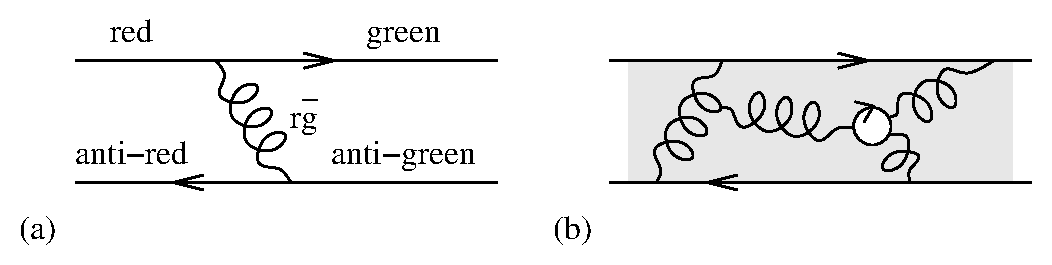
\includegraphics[width=\linewidth]{plots/gluejunk}
  \end{center}
  \caption{\label{gluejunk} (a) An example of a gluon as a force
  propagator and a carrier of color charge.  Directed lines are quarks
  and springs are gluons.  (b) An exchange between two quarks
  involving a complicated network of gluons and a light
  quark/anti-quark pair.  Grey shading indicates the sum of all such
  amplitudes.}
\end{figure}

A very successful model of the force between $b$ and $\bar{b}$
consists of a Coulomb-like potential at short distances (though \bork\
times stronger) and a linear potential at large distances (which
limits to a constant force of about 14 tons), as illustrated in
Figure~\ref{cornellpotential}(a).  At large distances, a string of
self-interacting gluons, stretched between the two quarks, is
responsible for the linear component.  This string will generate a
real quark/anti-quark pair and snap if stretched with sufficient
energy.  There are three $J=1$ solutions to the Schr\"odinger equation
below this threshold: they are labeled \us, \uss, and \usss.  States
above this threshold have a very different pattern of decay modes and
are beyond the scope of this study.

\begin{figure}[p]
  \begin{center}
    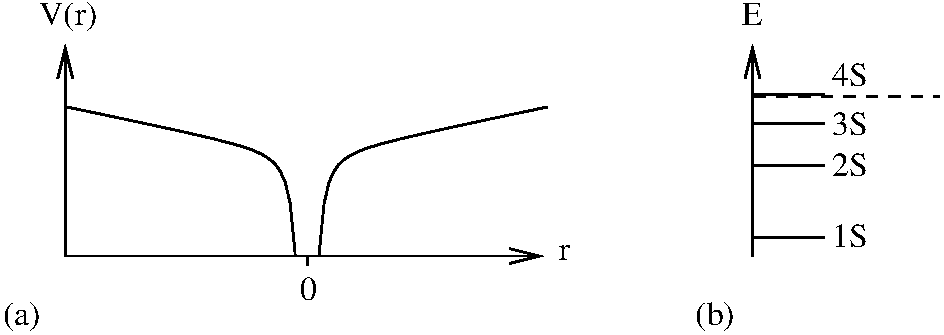
\includegraphics[width=0.8\linewidth]{plots/cornellpotential}
  \end{center}
  \caption{\label{cornellpotential} (a) Schematic of the potential
  energy between two quarks as a function of separation.  (b)
  Quantitative level diagram of $J=1$ $b\bar{b}$ solutions (\ups).
  The $\Upsilon(4S)$ lies just above the string-breaking threshold
  (dashed line).}
\end{figure}

These three mass eigenstates are the bottomonium equivalent of atomic
energy levels--- discrete lines of allowed mass-energies.  But, just
as in atomic spectra, the short lifetimes of these states imply a
broadening of their spectral lines: they are not perfect
time-independent solutions.  The full-width of an \ups\ resonance at
half-maximum, $\Gamma$, is equal to its decay rate, in analogy with
excited atomic resonances.  If we partition the \ups\ decays into
distinguishable modes, one being $\Upsilon \to e^+e^-$, the total
decay rate is a sum of those modes.  Hence, $\Gamma_{ee} = \Gamma \,
{\mathcal B}_{ee}$, where \gee\ is the di-electron width and \bee\ is
the fraction of \ups\ mesons that decay to \ee, that is, the branching
fraction to \ee.
  
The \ups\ meson decays into \ee\ by $b\bar{b}$ annihilation
(Figure~\ref{diagramgee}), which is a point-like interaction.  The $b$
and the $\bar{b}$ must fluctuate to the same point in space for the
reaction to proceed.  This probability, which is the square of the
$b\bar{b}$ spatial wavefunction evaluated at the origin
($|\psi(0,0,0)|^2$), is therefore a factor in \gee.
\begin{equation}
  \borkborkbork
  \label{eqn:waveatorigin}
\end{equation}
where $\alpha$ is the electromagnetic fine structure constant and
$M_\Upsilon$ is the \ups\ mass.  This is a non-relativistic
approximation: relativistic corrections replace the wavefunction at
the origin with an integral of values very close to the origin.
Because of this dependence on knowledge of the $b\bar{b}$
wavefunction, and therefore the potential, a first-principles
calculation \gee\ will require non-perturbative QCD.

\begin{figure}[p]
  \begin{center}
    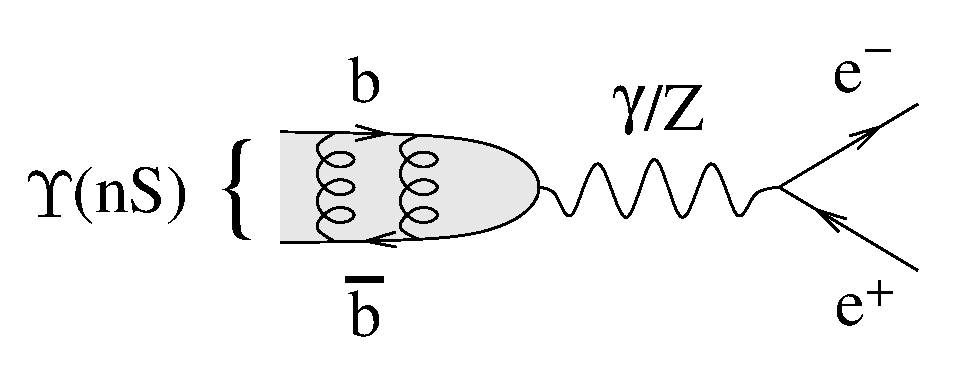
\includegraphics[width=0.5\linewidth]{plots/diagramgee}
  \end{center}
  \caption{\label{diagramgee} Decay diagram of $\Upsilon(nS)$ to \ee.
  The $Z^0$ contribution is 1.5\% of the total rate.}
\end{figure}

\section{Lattice QCD}

Feynman path integrals provide a general approach to quantum field
theory that don't rely on a perturbative expansion.  In this
formalism, the amplitude of a process is calculated as a weighted sum
of all possible ways it can proceed.  The value of every field at
every point in space in the initial state is allowed to vary as an
arbitrary function of time to the final state, and these paths are
weighted by their action.  This is a generalization of Lagrange's
method in classical physics, in which the true path is the one which
minimizes action.  In quantum physics, all paths which nearly minimize
action contribute to the amplitude of a process (Figure~\ref{pathintegrals}(a)).

\begin{figure}[p]
  \begin{center}
    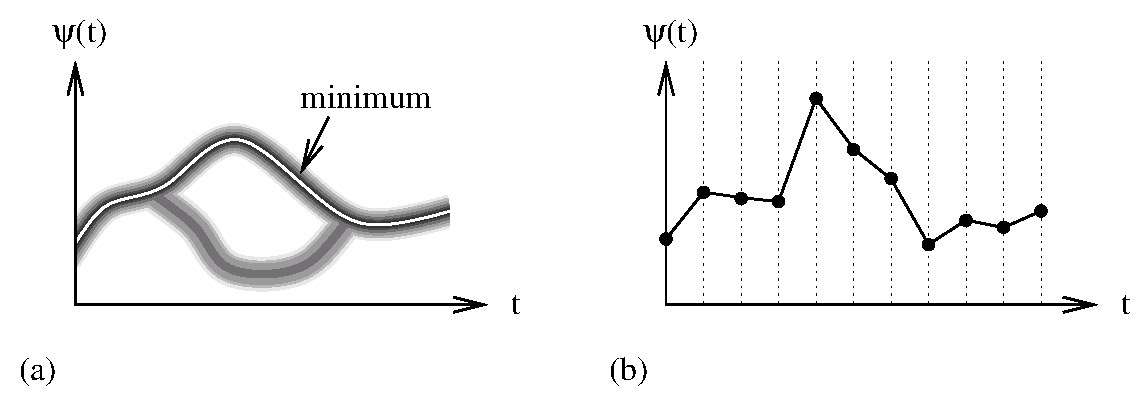
\includegraphics[width=\linewidth]{plots/pathintegrals}
  \end{center}
  \caption{\label{pathintegrals} (a) Paths in field strength ($\psi$)
  versus time.  The minimum (white) is the classical solution and the
  path which contributes the most to the quantum amplitude; shades of
  grey represent other quantum paths with smaller contributions to the
  total amplitude.  (b) A path approximated by a discrete time
  sequence.}
\end{figure}

To calculate a sum over a set of arbitrary paths, one must discretize
space-time into time slices and space cubes.  The path of a field
value in a space cube from the initial state to the final state is a
sequence of values for each time slice (Figure~\ref{pathintegrals}(b)).
A sequence of $N$ values is a vector in an $N$-dimensional vector
space: the weighting factor is integrated over these vector spaces.
To obtain a realistic result, one must afterward limit the
discretization scale to zero.

In general, realistic problems like QCD, the integral will not be
analytic and must be solved by numerical integration.  The integral
will have a fixed number of dimensions, which implies a fixed
discretization of space-time that can only be lifted by extrapolating
several calculations toward zero lattice size.  This discretization is
the lattice of Lattice QCD.  Quark field values are represented on a
four-dimensional lattice of space-time points with gluon field values
on the edges connecting them.

This is a very computationally intensive problem, since the number of
dimensions in the integral scales with the number of grid points, and
one must maximize the number of grid points to extrapolate to the
continuum limit.  Over the past 30 years, theorists have improved the
algorithms of Lattice QCD and sought approximations to make realistic
calculations tractable.

The most time-consuming part of most Lattice QCD calculations is the
polarization of the vacuum by light quarks.  In terms of Feynman
diagrams, these are interruptions of a gluon propagator by loops of
$u\bar{u}$, $d\bar{d}$ and $s\bar{s}$ pairs, which can be ignored or
suppressed by assuming infinite or very heavy up, down, and strange
quark masses.  This approximation is known as the quenched
approximation, and it permits calculations with 10--20\% systematic
uncertainties.

This situation was dramatically improved in the late 1990's by the
development of new algorithms based on the Symanzik-improved
staggered-quark formalism.  These algorithms are by far the most
efficient known, and the formalism features an exact chiral symmetry
that particularly benefits simulations with small light quark masses.
Realistic up and down quark masses are still out of reach, but
simulations using masses three times too large can be accurately
extrapolated with chiral perturbation theory.  Thus, ``unquenched''
calculations are now possible, resulting in the accurate prediction of
many masses and decay rates, as demonstrated in Figure~\ref{latticevictory}.

\begin{figure}[p]
  \begin{center}
    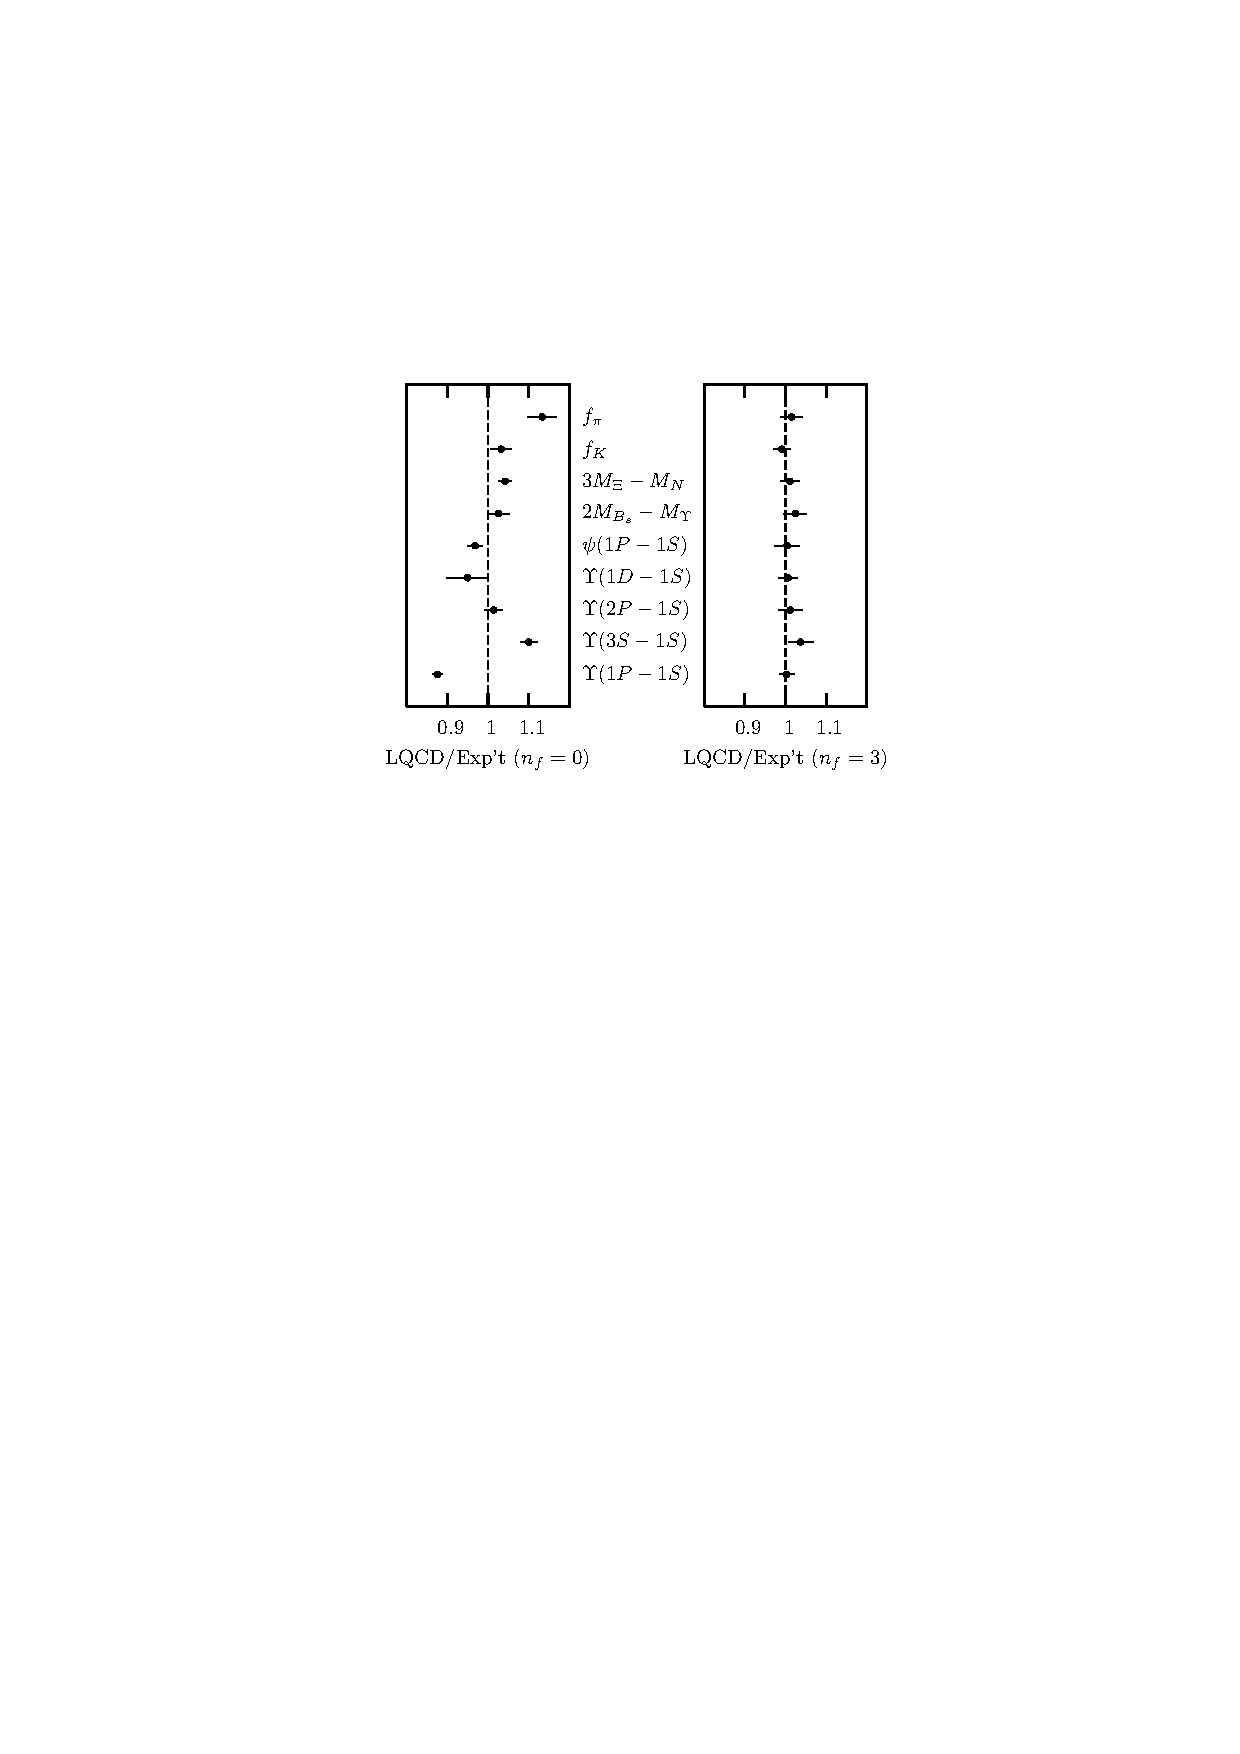
\includegraphics[width=\linewidth]{plots/latticevictory}
  \end{center}
  \caption{\label{latticevictory} Lattice QCD calculations divided by
  experimental measurements for nine quantities, without and with
  quark vacuum polarization (left and right panels, respectively).}
\end{figure}

This algorithmic speed comes at a conceptual price: the
staggered-quark formalism introduces four equivalent species of each
quark field, called ``tastes.''  These are artifacts of the formalism
and are unrelated to quark flavor.  Each of these tastes contributes
to the vacuum polarization, resulting in loop contributions which are
four times too large.  To correct for this, the quark determinant in
the action is replaced by its fourth root, a procedure which is
rigorous in the free-field theory and in perturbative QCD, but
introduces violations of Lorentz symmetry at short distances in the
lattice simulation.  Although these non-physical effects can be
removed by interpolating between the lattice points with perturbative
QCD, this issue makes the new algorithms controversial, and it is one
aspect that will be tested by confrontations with experiment.

The di-electron width may be determined from \ups\ simulations by
extracting the $b\bar{b}$ wavefunction at the origin and applying
Equation~\ref{eqn:waveatorigin}.  In a path integral context, the
wavefunction is the quark field amplitude.  These simulations employ a
non-relativistic QCD action with relativistic corrections, because the
de Broglie wavelength of a massive $b$ quark would require
impractically narrow time slices.

Simulations of the \ups\ mesons have been generated by the UKQCD
collaboration, but the determination of \gee\ from them is not yet
complete.  To properly calculate \gee, one needs to correct the
lattice wavefunction for discretization effects, which are on the
order of the Strong coupling constant, about 20\%.  This calculation
is in progress.  The largest terms in this correction cancel in ratios
of \gee: for instance, \gee\ from the \uss\ divided by \gee\ from the
\us\ can already be extracted with a 10\% uncertainty.
\begin{equation}
  \left. \frac{\Gamma_{ee}(2S)}{\Gamma_{ee}(1S)}
  \right|_\subs{UKQCD} = 0.43 \pm 0.04 \mbox{.}
  \label{eqn:latticeresult}
\end{equation}
This uncertainty is primarily due to residual discretization errors,
evident from the steep dependence of the result on lattice spacing
size (Figure~\ref{latticespacing}).  When the discretization
correction for each resonance has been calculated, the uncertainty in
this ratio should be only a few percent, while absolute \gee\ values
should have uncertainties on the 10\%-level.  This is why
experimentally precise values and ratios of \gee\ are both valuable.

\begin{figure}[p]
  \begin{center}
    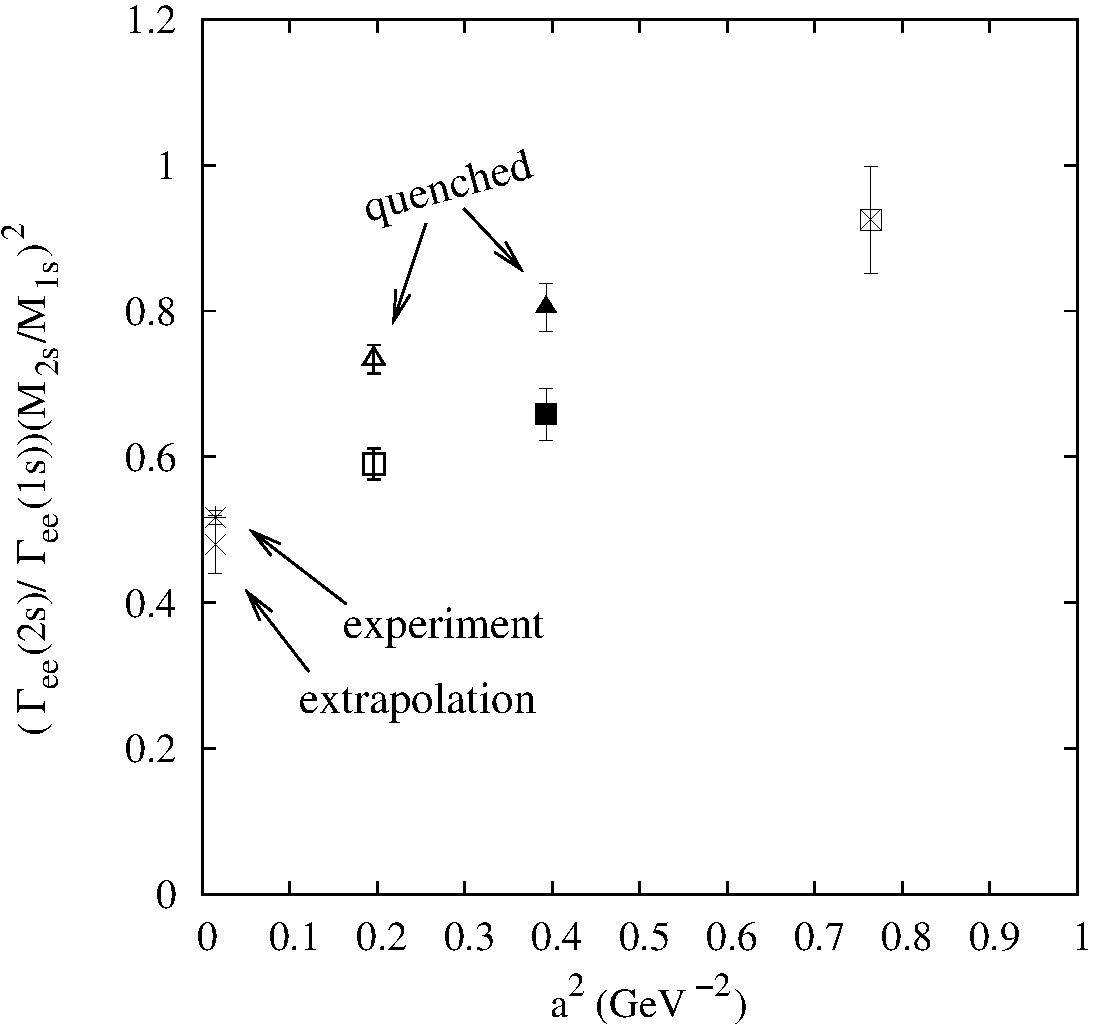
\includegraphics[width=\linewidth]{plots/latticespacing}
  \end{center}
  \caption{\label{latticespacing} UKQCD calculations of
  $\Gamma_{ee}(2S)/\Gamma_{ee}(1S)$ times the ratio of masses squared
  as a function of lattice grid size $a$.  Square data points
  represent calculations with realistic light quark masses (several
  times their natural values), and triangular points are quenched
  (infinite light quark masses).}
\end{figure}

\section{Relationship to Electroweak Parameter Extraction}

Lattice verification of \gee\ is particularly significant for an
application of the technique to Electroweak physics.  Vertices in
Feynman diagrams that join a top quark, a down quark, and a $W$ boson
contribute an a priori unknown factor, \vtd, to the amplitude (Figure~\ref{vtdvertex}).  This parameter is essential for violation of
charge-parity (CP) symmetry: if \vtd\ were zero, the Standard Model
would be CP symmetric (exchanging particles for antiparticles and
mirror-transforming space would preserve all observables).  To
determine \vtd, one must resort to measurements of bound quark
systems, because bare quarks do not exist in nature.  The transition
rates for these systems depend on \vtd\ and QCD factors related to the
structure of the bound state.  Lattice QCD can calculate these
factors and extract \vtd.

\begin{figure}[t]
  \begin{center}
    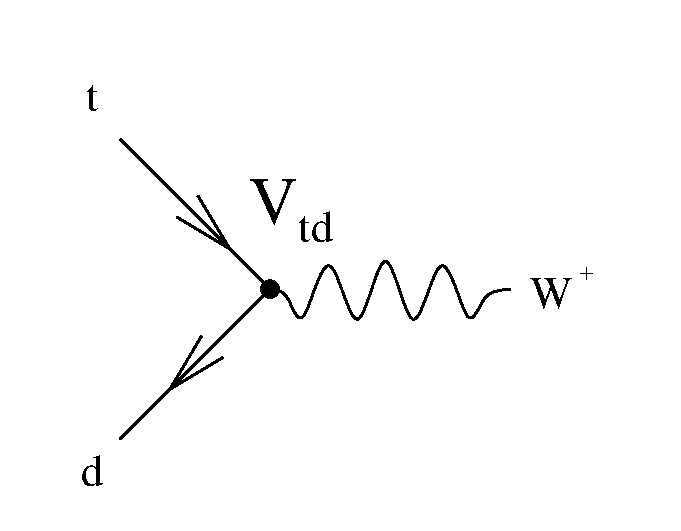
\includegraphics[width=0.5\linewidth]{plots/vtdvertex}
  \end{center}
  \caption{\label{vtdvertex} The vertex joining top, down, and
  $W^\pm$.}
\end{figure}

The most sensitive probe of \vtd\ is $B^0$-$\bar{B^0}$ mixing.  A
$B^0$ meson is a bound state of $d$ and $\bar{b}$, and a $\bar{B^0}$
meson is its charge conjugate, $b\bar{d}$.  These two mesons can mix,
that is, a $B^0$ can transform into a $\bar{B^0}$ and vice-versa,
through the diagram illustrated in Figure~\ref{bmixing}(a).  The heavy
top quark dominates in this loop and provides a factor of \vtd\ for
each vertex with a down quark.  The rate of this process is extremely
well-known: \bork\ \PM\ \bork\ ps\inv, a 1\% measurement.

\begin{figure}[p]
  \begin{center}
    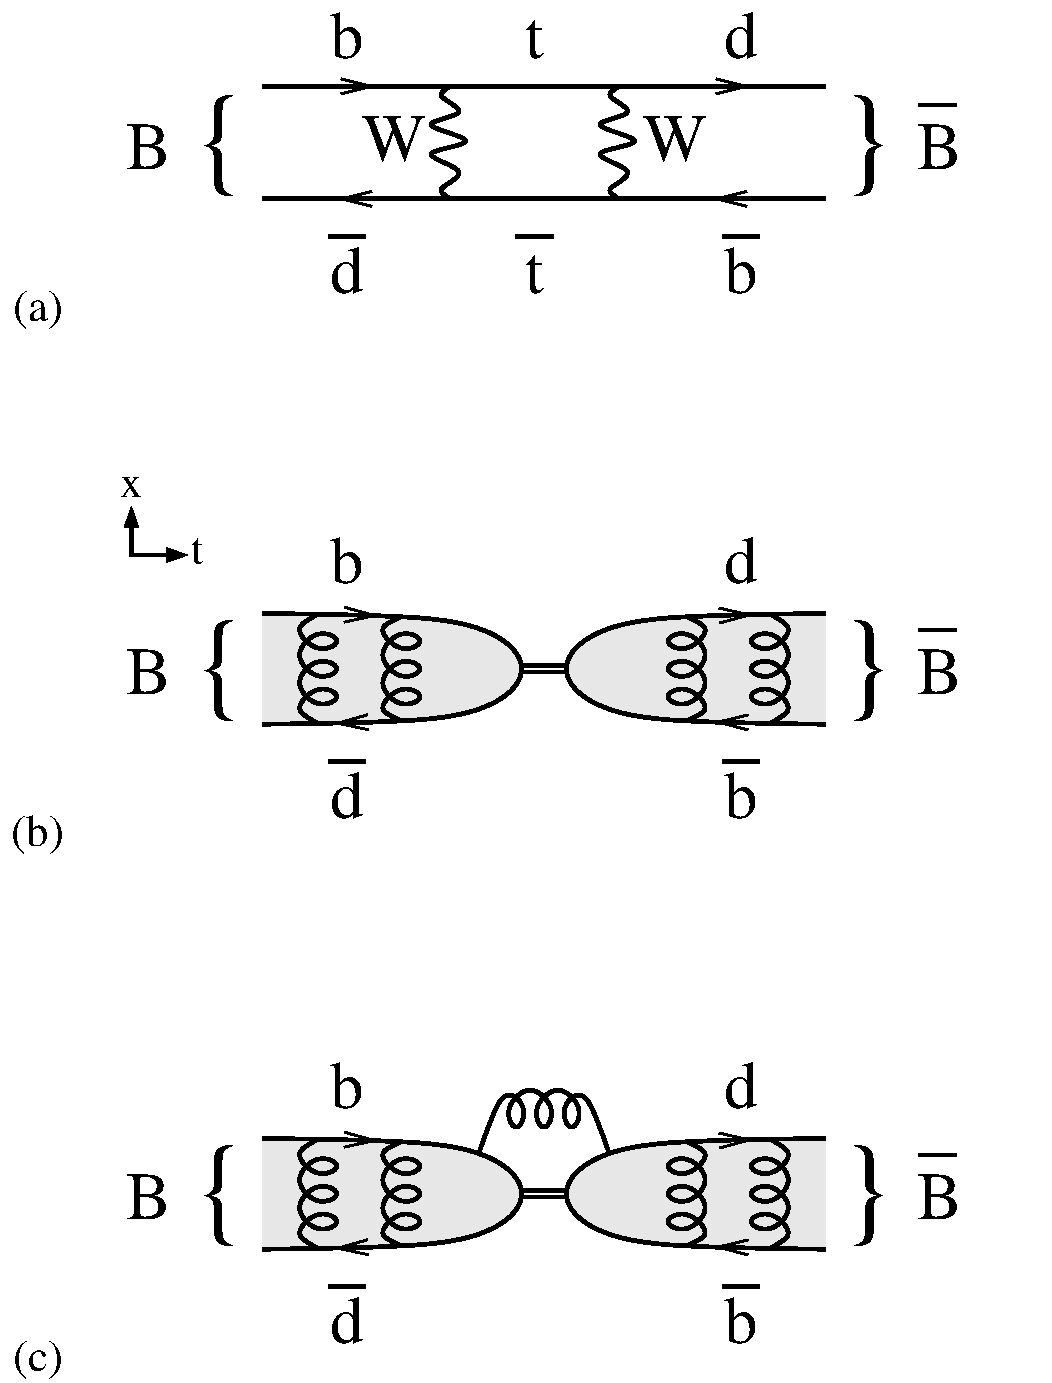
\includegraphics[width=0.7\linewidth]{plots/bmixing}
  \end{center}
  \caption{\label{bmixing} (a) One of the two diagrams dominating
  $B^0$-$\bar{B^0}$ mixing (the other exchanges $t \leftrightarrow
  W$).  (b) The same diagram emphasizing the Strong force between the
  quarks and the relative size of the $t$-$W$ loop.  (c) Diagrams that
  contribute to the Bag parameter, which is not a part of $f_B$.}
\end{figure}

Despite this precision, the \vtd\ extraction has 20\% uncertainties
from Strong interactions.  The $W$-$t$ loop in this diagram represents
a very short-range process ($\sim$0.001~fm).  By comparison, the
average distance between the $b$ and $\bar{d}$ quarks is set by the
QCD potential ($\sim$fm), just as it is for $b\bar{b}$ in the \ups\
meson.  As a space-time diagram, the $B^0$-$\bar{B^0}$ mixing process
would look a little more like Figure~\ref{bmixing}(b).  Just as in
\gee, the rate of $B^0$-$\bar{B^0}$ mixing is determined by the
probability that the two quarks will fluctuate to the same point in
space, and this probability is characterized by the $B$ meson decay
constant $f_B$.
\begin{equation}
  \Gamma(B \to \bar{B}) = \mbox{(known factors)} \times \bigg|
  \underbrace{{f_B}^2 B_B}_\subs{QCD} \times {V_{td}}^2 \bigg|^2
  \mbox{.}
\end{equation}
The $B^0$-$\bar{B^0}$ mixing amplitude depends on two factors of
$f_B$, one from the $B^0$ wavefunction and the other from $\bar{B^0}$
(see Figure~\ref{bmixing}(b)).  Another factor, known as the Bag
parameter $B_B$, corrects for gluons connecting the $B^0$ and
$\bar{B^0}$.  Its uncertainty is more easily controlled.  Our
knowledge of \vtd\ is therefore dominated by the uncertainty in $f_B$.

In principle, one can measure $f_B$ experimentally through $B^+ \to
\mu^+ \nu$ or $\tau^+ \nu$, illustrated in Figure~\ref{btomunu}.  The
charged $B^+$ has different quark content from the neutral $B^0$, but
its decay rate depends on $f_B$ because up and down quark masses are
both much smaller than the bottom quark mass, and flavors do not enter
the QCD calculation.  Unfortunately, this process is suppressed by the
helicity of the $\tau^+ \nu$ final state, to the extent that it has
yet to be observed in \bork\ zillion $B^\pm$ decays at BaBar and Belle.
Given the low rate of this decay, it will take a long time to
accumulate enough data to make a statistically significant measurement
of $f_B$.

\begin{figure}[p]
  \begin{center}
    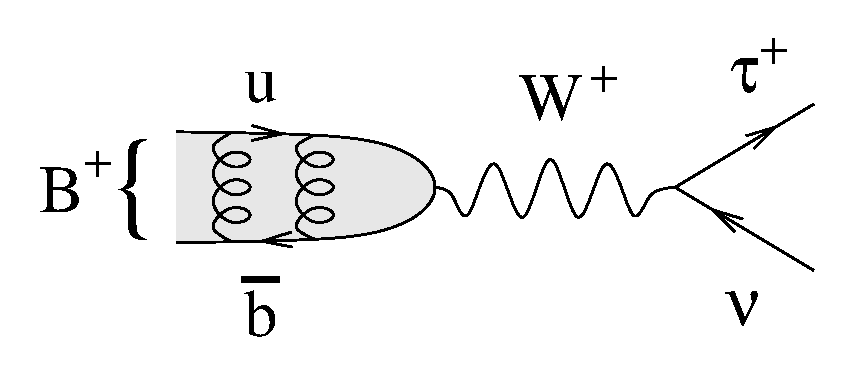
\includegraphics[width=0.5\linewidth]{plots/btomunu}
  \end{center}
  \caption{\label{btomunu} Decay diagram of $B^+ \to \tau^+ \nu$.}
\end{figure}

The $B$ decay constant can be extracted from Lattice QCD simulations
of $B$ mesons in much the same way as \gee\ is from \ups\ simulations:
by sampling the wavefunction at the origin.  The discretization issues
and corrections to this calculation are also very analogous to \gee.
Preliminary results by the UKQCD collaboration find $f_B$ = \bork\ and
are plotted in Figure~\ref{fbresults}.  Like \gee, these results are
in progress.

\begin{figure}[p]
  \begin{center}
    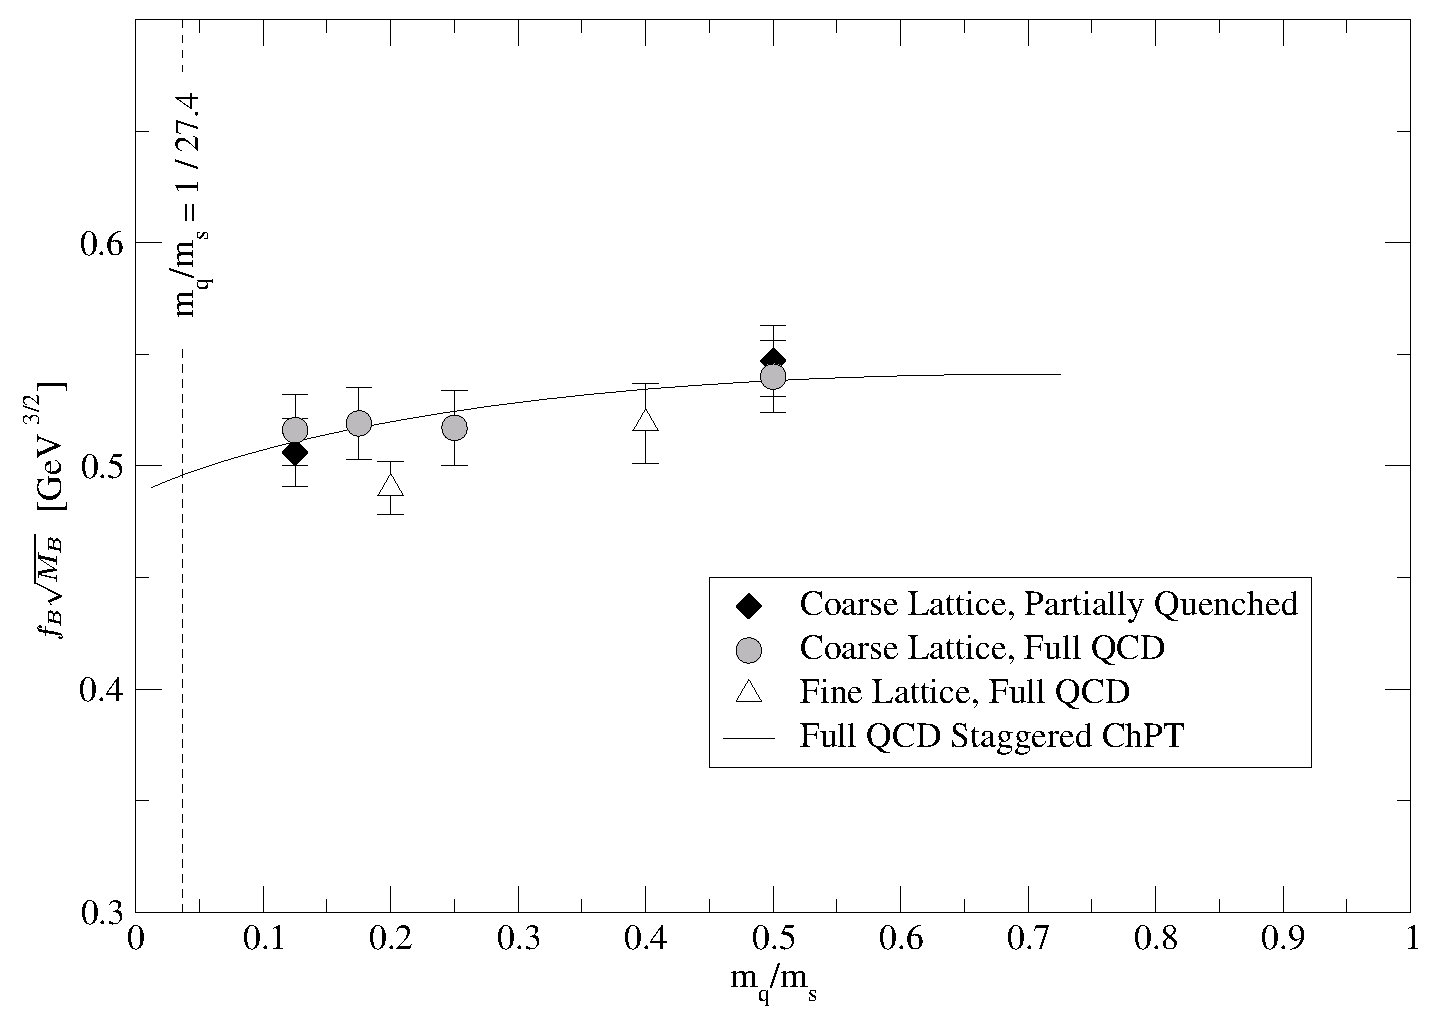
\includegraphics[width=\linewidth]{plots/fbresults}
  \end{center}
  \caption{\label{fbresults} UKQCD calculations of $f_B \sqrt{M_B}$ as
  a function of light quark masses used in the simulations.  The solid
  curve extrapolates from the simulations to the natural $m_q/m_s$ of
  1/27.4.}
\end{figure}

Lattice calculations of $f_B$ would be viewed with suspicion if
calculations of \gee\ do not match experiment at a comparable level of
precision.  From the lattice's perspective, the only difference
between these two calculations is the mass of one of the two quarks: a
bottom quark is replaced by a light quark.  This is not a trivial
distinction: it is also worthwhile checking the lattice calculation of
the $D$ meson decay constant, in which a charm quark and a light quark
annihilate, with experimental results that are now becoming available.
The $D$ meson is a heavy/light quark combination, just like the $B$
meson, so $f_D$ is physically more analogous to $f_B$ than \gee\ is.
However, the $D$ meson is a more relativistic system, the charm quark
being four times lighter than bottom, so instead of simulating a
non-relativistic QCD action for charm quarks, $D$ simulations use a
relativistic approximation known as the FermiLab action.  Thus, the
calculation of \gee\ is, in some important technical aspects, more
similar to the calculation of $f_B$ than $f_D$ is.  We believe that
QCD is the correct description of the Strong force, so experimental
checks of Lattice QCD will primarily be testing the implementation of
QCD on the lattice, rather than QCD itself.  Thus, experimental
verification of \gee\ calculations are key to our confidence in $f_B$
calculations, and therefore the value of \vtd.

\chapter{Measurement Technique}
\label{chp:technique}

\section{Scans of \boldmath \ups\ Resonance Production}

To determine the decay rate of $\Upsilon \to e^+e^-$, we use a special
strategy available to \ee\ colliders: we measure the total
cross-section of $e^+e^- \to \Upsilon$, the time-reversed process.
This cross-section, which quantifies the probability of \ups\
production independently of the \ee\ collision luminosity, is related
to the $b\bar{b}$ wavefunction at the origin for the same reason as
\gee\ (Figure~\ref{timereversed}).
\begin{equation}
  \borkborkbork
  \label{eqn:crosssecwaveorigin}
\end{equation}
where the $dE_\subs{CM}$ integration is performed over \ee\
center-of-mass energies.  To obtain \gee\ in terms of $\int
\sigma(e^+e^- \to \Upsilon) \, dE_\subs{CM}$, we combine the above
with Equation~\ref{eqn:waveatorigin}.
\begin{equation}
  \Gamma_{ee} = \frac{{M_\Upsilon}^2}{6\pi^2} \int \sigma(e^+e^- \to
  \Upsilon) \, dE_\subs{CM} \mbox{.}
  \label{eqn:gee}
\end{equation}
This is more general than Equations \ref{eqn:waveatorigin} and
\ref{eqn:crosssecwaveorigin}, which only apply in the non-relativistic
limit.  In the fully relativistic case, $|\psi(0,0,0)|^2$ must be
replaced with an integral of wavefunction values near the origin,
which cancels in Equation~\ref{eqn:gee}.

\begin{figure}[p]
  \begin{center}
    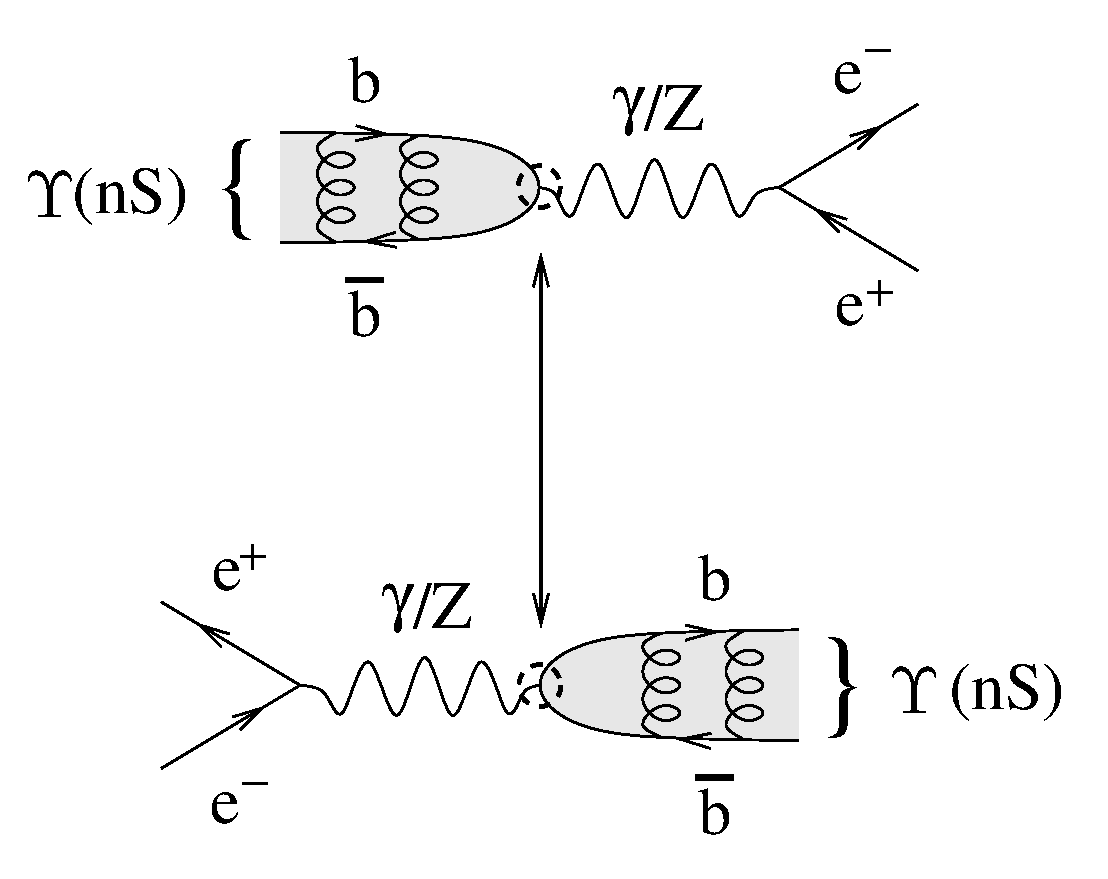
\includegraphics[width=0.6\linewidth]{plots/timereversed}
  \end{center}
  \caption{\label{timereversed} Diagrams of $\Upsilon \to e^+e^-$ and
  $e^+e^- \to \Upsilon$.  Both feature the same
  $b$-$\bar{b}$-$\gamma/Z^0$ vertex whose rate is set by
  $|\psi(0,0,0)|^2$.}
\end{figure}

This may seem like a very indirect way of measuring \gee.  Why do we
not count $\Upsilon \to e^+e^-$ decays relative to the number of \ups\
mesons produced, for instance?  The reason is because such a fraction
would be \bee, rather than the decay rate.  We would need to multiply
by $\Gamma$, the distribution of \ups\ masses, to determine \gee, and
this is experimentally inaccessible: $\Gamma$ is on the order of 50
keV, which is about a hundred times narrower than the beam energy
spread of an \ee\ collider and a thousand times narrower than detector
resolution.  Equation~\ref{eqn:gee} provides direct access to \gee,
which, as a collateral benefit, can be combined with \bee\ to obtain
$\Gamma$.

To evaluate $\int \sigma(e^+e^- \to \Upsilon) \, dE_\subs{CM}$, we
sample the \ups\ cross-section at \ee\ energies near the \ups\ masses
(9.4--10.4 GeV) and fit a curve to these lineshapes.  We then
integrate this curve analytically.  To construct our fit function, we
begin with the natural lineshape of the \us, \uss, and \usss\
resonances, a Breit-Wigner:
\begin{equation}
  \sigma(e^+e^- \to \Upsilon)(E_\subs{CM}) = \left(
  \frac{6\pi^2}{{M_\Upsilon}^2} \, \Gamma_{ee} \right)
  \frac{\Gamma/2\pi^2}{(E_\subs{CM} - M_\Upsilon)^2 + (\Gamma/2)^2} \mbox{.}
  \label{eqn:breitwigner}
\end{equation}
The observed spectrum is smeared by a unit Gaussian spread in incident
beam energies ($\sim$4 MeV), as discussed above.  We represent this
smearing by a convolution, but the total integral is unchanged.

The high-energy side of the lineshape is also distorted by
initial-state radiation (ISR): $e^+e^- \to \Upsilon$ events are hard
to distinguish from $e^+e^- \to \gamma \Upsilon$ for sufficiently
small photon energies $E_\gamma$.  These events add to the
cross-section, and contribute a high-energy tail that falls of as
$1/E_\gamma$, causing the integral to diverge.  We could introduce an
artificial cut-off, but then the \gee\ we report would be a function
of that cut-off.  Instead, we include the ISR distortion in our fit
function to match the data, but report the integral with no ISR
contribution, a procedure depicted in Figure~\ref{cartoon}.  This
means that $\sigma(e^+e^- \to \Upsilon)$ in Equation~\ref{eqn:gee}
represents the \ups\ cross-section with no ISR photons at all, and the
\gee\ we derive is devoid of final-state radiation ($\Upsilon \to
\gamma e^+e^-$).

\begin{figure}[p]
  \begin{center}
    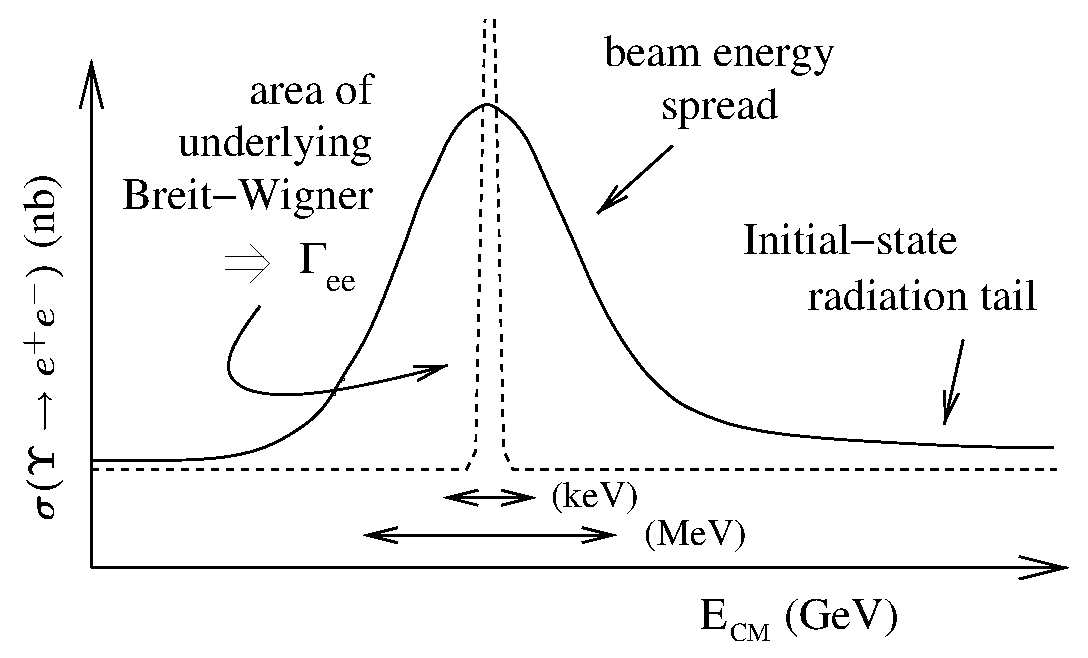
\includegraphics[width=0.7\linewidth]{plots/cartoon}
  \end{center}
  \caption{\label{cartoon} The anatomy of an \ups\ lineshape scan
  (cross-section versus center-of-mass energy), including the natural
  lineshape (dashed peak), beam energy spread and ISR tail (solid),
  and backgrounds (vertical offset).}
\end{figure}

In addition to $e^+e^- \to \Upsilon$ and $\gamma \Upsilon$,
electron-positron collisions in the 9.4--10.4 GeV range can also
undergo the following continuum processes, which also contribute to
the observed cross-section:  \renewcommand{\labelenumi}{\alph{enumi}.}
\begin{enumerate}

  \item fermion pairs purely through annihilation ($s$-channel,
    Figure~\ref{continuum}(a)),

  \item Bhabha \ee\ through annihilation ($s$-channel) and Coulomb
    scattering \\ (\mbox{$t$-channel,} Figure~\ref{continuum}(b)),

  \item \gamgam\ through annihilation (Figure~\ref{continuum}(c)), and

  \item $e^+e^- X$ via the fusion of two virtual photons from a
    grazing collision (Figure~\ref{continuum}(d)).

\end{enumerate}
Muon- and tau-pair cross-sections are about 0.8(?)~nb, and \qqbar\ are
about 3(?)~nb, decreasing with center-of-mass energy as $1/s$ ($s =
{E_\subs{CM}}^2$).  Bhabha events are by far the most abundant; in
fact, the Bhabha cross-section diverges if glancing-angle scatters are
included.  The \gamgam\ cross-section diverges also, but less rapidly
with angle.  Bhabha and \gamgam\ cross-sections both decrease as
$1/s$.  The last process, two-photon fusion, generates low-momentum
hadronic particles $X$ and two electrons, at least one of which grazes
the incident beam-line.  The two-photon fusion cross-section increases
with center-of-mass energy, but very slowly, as $\log s$.  Some of
these non-\ups\ processes can be hard to distinguish or are
indistinguishable from \ups\ events, and therefore can be confused
with signal.  Fortunately, the continuum cross-section depends on
\ecm\ much more slowly than \ups\ does, so the \ups\ peak appears to
stand on a flat continuum plateau, also depicted in
Figure~\ref{cartoon}.  We add terms to the fit function to accommodate
these effects as well.

\begin{figure}[p]
  \begin{center}
    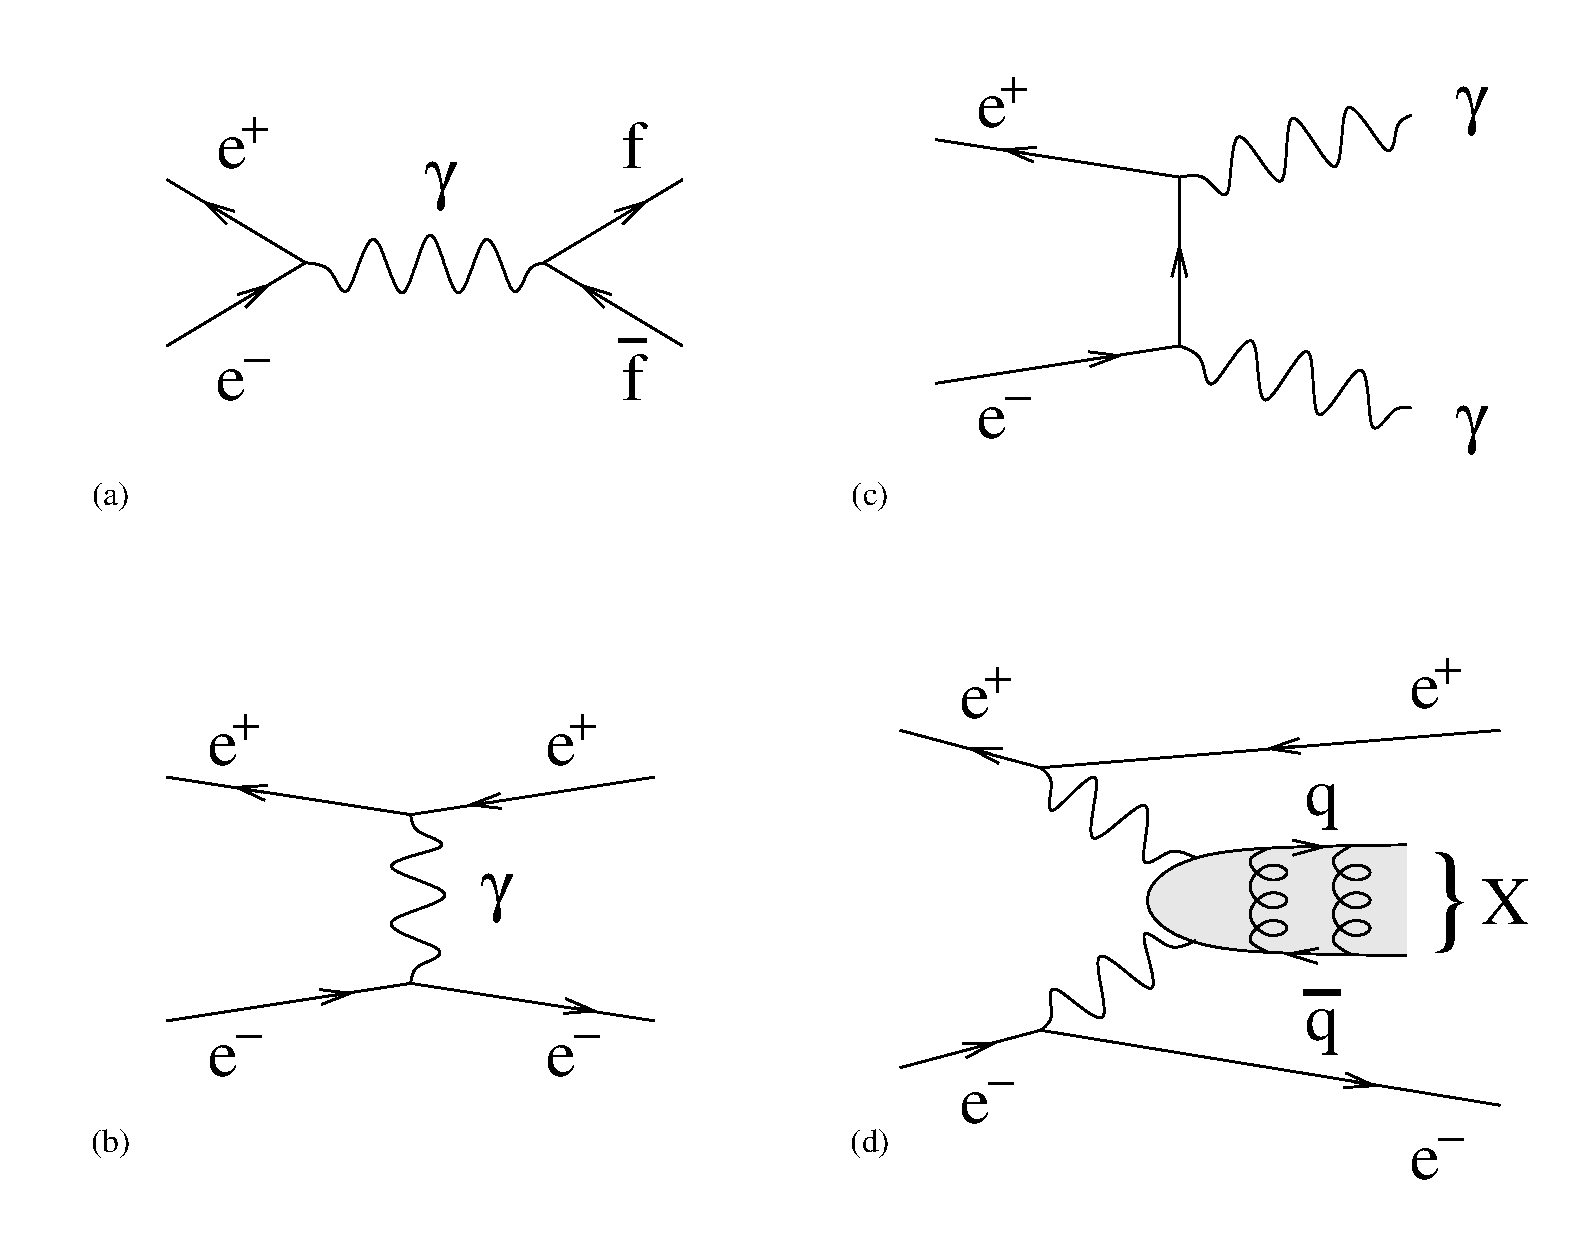
\includegraphics[width=\linewidth]{plots/continuum}
  \end{center}
  \caption{\label{continuum} Survey of continuum backgrounds: (a)
  $s$-channel fermion pair production, $f\bar{f}$ may be \ee, \mumu,
  \tautau, or \qqbar.  (b) $t$-channel exchange which dominates Bhabha
  (\ee) scattering.  (c) \ee\ annihilation into two real photons (the
  other, undrawn diagram simply exchanges the identity of the two
  outgoing photons).  (d) Fusion of two virtual photons into a
  low-momentum hadronic state accompanied by high-energy \ee.}
\end{figure}

When a continuum final state is truly indistinguishable from an \ups\
decay, as is the case for $e^+e^- \to q\bar{q}$ and $e^+e^- \to
\Upsilon \to q\bar{q}$, the cross-sections don't simply add.  The
complex amplitudes for these processes add, the square of which is
proportional to cross-section: \label{sec:earlyinterference}
%
\newcommand{\res}{{\mbox{\scriptsize res}}}
\newcommand{\cont}{{\mbox{\scriptsize cont}}}
\newcommand{\inter}{{\mbox{\scriptsize int}}}
\newcommand{\aye}{{\mathcal A}}
\begin{eqnarray}
  \hspace{-0.3 cm} \sigma_{\res+\cont}(E_\subs{CM}) &\propto& \big| \aye_\res + \aye_\cont \big|^2 =
  \big| \aye_\res \big|^2 + \big| \aye_\cont \big|^2 + 2 {\mathcal Re}({\aye_\res}^* \aye_\cont) \\
  &=& \sigma_\res(E_\subs{CM}) + \sigma_\cont(E_\subs{CM}) + \tilde{\sigma}_\inter(E_\subs{CM})
  \label{eqn:rescontinter}
\end{eqnarray}
where $\sigma$ denotes cross-section and $\aye$ amplitude, ``res'' for
the resonant (\ups) contribution and ``cont'' for the continuum.  The
interference term, $\tilde{\sigma}_\inter$, is a function of \ecm, like the
familiar $\sigma_\res$ and $\sigma_\cont$, but it can be negative and
sometimes larger than $\sigma_\res$.  That is, introducing another way
for \ee\ to produce \qqbar\ can actually decrease the \qqbar\
cross-section!  We calculate this interference term from a
Breit-Wigner amplitude (Feynman propagator) of the form
\begin{equation}
  \aye_\res \propto \frac{1}{E_\subs{CM} - M_\Upsilon + i\Gamma/2}
\end{equation}
and a constant continuum with constant phase $\phi_0$ (with respect to
the resonance phase at $E_\subs{CM} \ll M_\Upsilon$).  We find
\begin{eqnarray}
  \tilde{\sigma}_\inter(E_\subs{CM}) &=& \alpha_\subs{int} \, \sigma_\subs{res}(E_\subs{CM}) \,
  \left(2 \frac{E_\subs{CM} - M_\Upsilon}{\Gamma} \cos \phi_0 + \sin
  \phi_0 \right) \\
  \mbox{where } \alpha_\subs{int} &=& \sqrt{\Gamma_f \, \sigma_\cont \, ({M_\Upsilon}^2 / 3 \Gamma_{ee})}
  \label{eqn:yint}
\end{eqnarray}
and $\Gamma_f$ is the rate of \ups\ decay to the final state (in this
case, \qqbar).  If only $\Upsilon \to q\bar{q}$ decays interfere with
continuum \qqbar, then $\alpha_\subs{int}$ is \bork.  Note that if $\phi_0
= 0$, $\tilde{\sigma}_\inter < 0$ below $M_\Upsilon$ and $\tilde{\sigma}_\inter > 0$
above $M_\Upsilon$, and if $\phi_0 = \pm\pi/2$, $\tilde{\sigma}_\inter$ will have
exactly the same energy dependence as $\sigma_\res$, and thus be
indistinguishable from the \ups\ cross-section itself.  Continuum
Bhabhas, \mumu, \tautau, and \qqbar\ all have $\phi_0 = 0$.  [Justify!]

\section{\boldmath \ups\ Final States and Hadronic Cross-section}

In our \ee\ collisions, \ups\ mesons are produced nearly at rest and
immediately decay.  We only ever observe the \ups\ decay products.  An
\ups\ may decay into
\renewcommand{\labelenumi}{\alph{enumi}.}
\begin{enumerate}

  \item leptonic final states: \ee, \mumu, and \tautau, through an
    $s$-channel virtual photon (or $Z^0$, with 1\% contribution),

  \item hadronic final states via the hadronization of \qqbar, \ggg,
    or \gggamma,

  \item lower-mass $b\bar{b}$ states, accompanied by pions or photons,

  \item neutrino pairs exclusively through $Z^0$, and

  \item possibly other, exotic, modes.

\end{enumerate}

The \mumu\ branching fractions, \bmm, have been measured with 2--5\%
precision for \us, \uss, and \usss, and \ee\ and \tautau\ are expected
to have the same decay amplitudes.  Thus, the branching fractions,
\bee, \bmm, and \btt, are nearly equal, with only a tiny correction
from lepton mass, which is 0.05\% for the heavy $\tau$ lepton.  This
assumption is called Lepton Universality.

States containing bare quarks or gluons (partons), like \qqbar, \ggg,
and \gggamma, must hadronize before propagating to the detector.  That
is, strings of self-interacting gluons, stretched between the partons,
will generate new quark/anti-quark pairs when stretched sufficiently
far.  These new quarks will clothe the original partons, such that a
macroscopic detector will only ever observe mesons ($q\bar{q}$ bound
states) and baryons ($qqq$ or $\bar{q}\bar{q}\bar{q}$).  Hadronization
is a random process, leading to a broad spectrum of event topologies,
with as many as twenty particles in the final state.  Most \ups\
mesons decay hadronically.

Only the \uss\ and the \usss\ have appreciable decay rates to other
$b\bar{b}$ states.  These decays are the bottomonium equivalent of
atomic transitions, but in addition to emitting monoenergetic photons
in $\Delta J = 1$ decays, bottomonium can emit monoenergetic $\pi\pi$
(charged or neutral) and $\gamma\gamma$ when decaying with $\Delta J =
0$.  Figure~\ref{bbtransitions} plots the energy levels of the most
well-known $b\bar{b}$ states and the transitions between them.

\begin{figure}[p]
  \begin{center}
    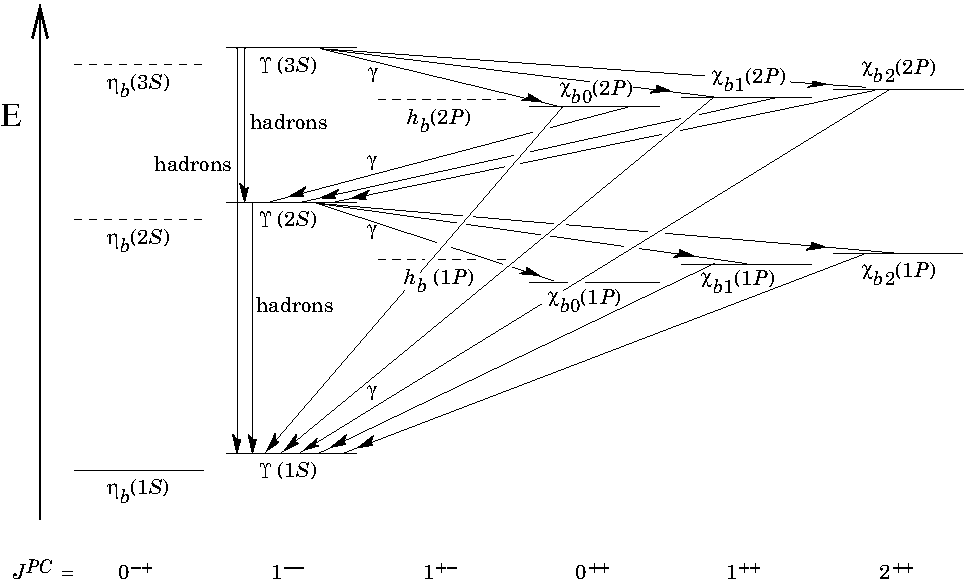
\includegraphics[height=0.7\linewidth, angle=90]{plots/bbtransitions}
  \end{center}
  \caption{\label{bbtransitions} States and transitions in the
  $b\bar{b}$ system.  Only $J=1$ \ups\ mesons are produced directly by
  \ee, and of those, only \uss\ and \usss\ decay significantly into
  lower $b\bar{b}$ states.}
\end{figure}

The \ups\ masses are about ten times smaller than the $Z^0$ mass, so
$Z^0$ contributes to only about 1\% of the \ups's $s$-channel decays.
The rate of $\Upsilon \to \nu\bar{\nu}$ is therefore only about 0.2\%,
which is negligible at our level of precision.  [Check all the $Z^0$,
$\nu\bar{\nu}$ numbers.  Doesn't $(M_\Upsilon/M_Z)^2$ apply only to
the $s$-channel part, which is only $(3+R)$\bmm?]

Finally, we do not exclude the possibility that unknown \ups\ decays
exist, or that their branching fractions are larger than a few
percent.  These modes may resemble hadronic decays, or have exotic
signatures that have been overlooked.

For the sake of this analysis, we will classify \ups\ decay modes as
``leptonic,'' meaning \ee, \mumu, and \tautau\ exclusively (no
$\nu\bar{\nu}$), or ``hadronic,'' meaning everything else.  By this
designation, there are ``hadronic'' final states that contain no
hadrons at all, such as the $\Upsilon(2S) \to \gamma \chi_{b1}(1P) \to
\gamma\gamma \Upsilon(1S) \to \gamma\gamma e^+e^-$ chain, $\Upsilon
\to \nu\bar{\nu}$, and $\Upsilon \to \mbox{\sc wimp }
\overline{\mbox{\sc wimp}}$ (where {\sc wimp}s are
cosmologically-motivated invisible particles).  This classification is
convenient and has been used by previous \gee\ analyses.

Experimentally, the \ups\ cross-section is the number of $e^+e^- \to
\Upsilon$ events that occurred divided by the time-integrated
luminosity of the \ee\ beams.  To identify $e^+e^- \to \Upsilon$
events, we select events that look like hadronic \ups\ decays, because
the leptonic final states are hard to distinguish from continuum
backgrounds.  Thus, we count $e^+e^- \to \Upsilon \to \mbox{hadronic}$
events and our cross-section is $\sigma(e^+e^- \to \Upsilon \to
\mbox{hadronic})$.  This hadronic cross-section is a constant multiple
of the total cross-section
\begin{equation}
  \sigma(e^+e^- \to \Upsilon \to \mbox{hadronic}) = \sigma(e^+e^- \to
  \Upsilon) \times \Gamma_\subs{had} / \Gamma_\subs{tot}
\end{equation}
for all \ecm.  We fit our lineshape function to hadronic cross-section
versus \ecm\ data and thereby derive \geehadtot.  To obtain \gee, we
need to divide by ${\mathcal B}_\subs{had} =
\Gamma_\subs{had}/\Gamma_\subs{tot}$, which is $(1 - {\mathcal B}_{ee} -
{\mathcal B}_{\mu\mu} - {\mathcal B}_{\tau\tau})$ by definition.
Applying Lepton Universality, we use
\begin{equation}
  \Gamma_{ee} = \frac{\Gamma_{ee}\Gamma_\subs{had}/\Gamma_\subs{tot}}{1
  - 3 {\mathcal B}_{\mu\mu}}
  \label{eqn:geehadtot:to:gee}
\end{equation}
to take advantage of the well-measured \bmm.  With \gee, we again
assume ${\mathcal B}_{ee} = {\mathcal B}_{\mu\mu}$ to calculate
$\Gamma = \Gamma_{ee} / {\mathcal B}_{\mu\mu}$, and we estimate the
$b\bar{b}$ wavefunction at the origin with Equation~\ref{eqn:waveatorigin}.

The upcoming chapters will each present one aspect of the \geehadtot\
measurement.
\begin{description}

  \item[Chapter \ref{chp:hardware}] will describe the \ee\ collider
    and particle detector that were used to generate and count $e^+e^-
    \to \Upsilon \to \mbox{hadronic}$ events.

  \item[Chapter \ref{chp:backgrounds}] will define the $e^+e^- \to
    \Upsilon \to \mbox{hadronic}$ selection criteria and explain how
    non-\ups\ events are removed from that count.

  \item[Chapter \ref{chp:efficiency}] will derive the correction
    for hadronic \ups\ events missing from the sample, that is, the
    efficiency of the selection criteria.

  \item[Chapter \ref{chp:luminosity}] will explain how we measure
    integrated luminosity, thereby converting our hadronic event
    counts into hadronic cross-sections.

  \item[Chapter \ref{chp:beamenergy}] will show how we use
    cross-section data to put an upper limit on the uncertainty in
    beam energy measurements.

  \item[Chapter \ref{chp:fitting}] will describe the fit function and
    fit results in detail, and

  \item[Chapter \ref{chp:results}] will present all \geehadtot, \gee,
  $\Gamma$, and $|\psi(0,0,0)|^2$ results.

\end{description}

\chapter{Collider and Detector}
\label{chp:hardware}

\section{Cornell Electron Storage Ring}

Our electron-positron pairs were collided in the Cornell Electron
Storage Ring (CESR), a 768~m-circumference, symmetric storage ring
and collider in Ithaca,~NY.  This collider has demonstrated a very
broad capacity for \ee\ energies, from the $J/\psi$ region at
$E_\subs{beam} = E_\subs{CM}/2 =$ 1.5~GeV through the excited \ups\
states at 5.5~GeV.  The \us, \uss, and \usss\ masses, between 4.7 and
5.2~GeV, lie in CESR's optimal range.  In fact, scans of the \us\
through \usss\ are among the first data taken by CESR in 1979
(Figure~\ref{greetingsfromcesr}).

\begin{figure}[p]
  \begin{center}
    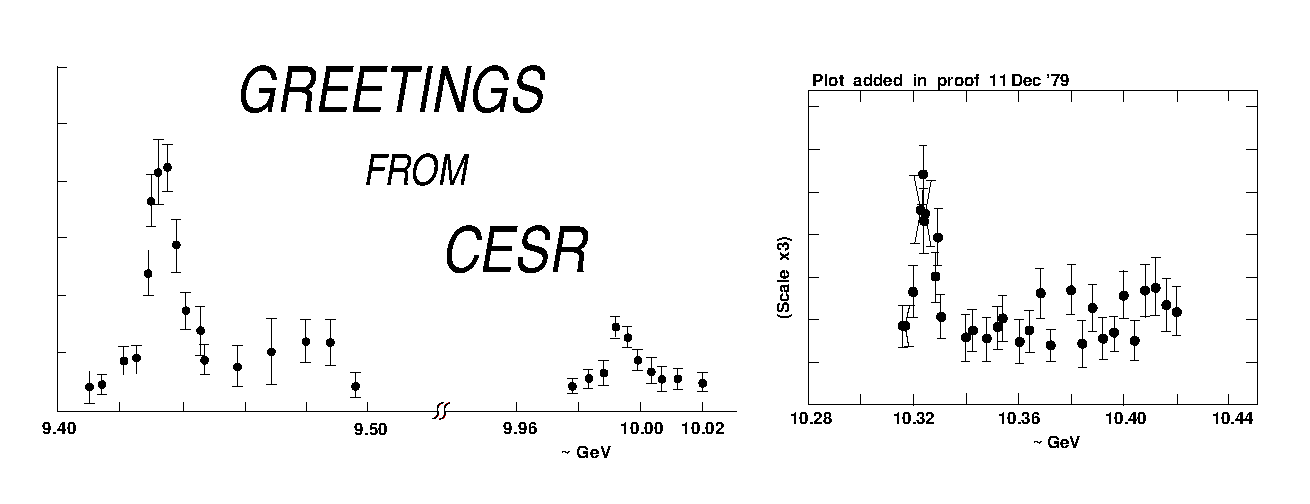
\includegraphics[width=\linewidth]{plots/greetingsfromcesr}
  \end{center}
  \caption{\label{greetingsfromcesr} Greeting card from CESR in 1979,
  demonstrating its success in colliding \ee\ at 10~GeV by scanning
  the lineshapes of the \us, \uss, and \usss\ (left to right).}
\end{figure}

Copper dipole magnets confine the beams to their orbits, interspersed
with quadrapole and sextapole magnets for focusing.  Superconducting
quadruples provide the final focusing of the beams before they
collide, only 30~cm from the interaction point, allowing the
collisions to reach instantaneous luminosities of
$10^{33}$~cm$^{-2}$~s\inv.  Like all synchrotrons, the beam is pulsed
to permit acceleration: beam bunches are timed to enter radio
frequency (RF) standing waves just when the electric field is maximal.
In CESR, nine trains of five bunches circulate in the ring at once,
with 1.15$\times 10^{10}$ particles per bunch.  Both the electron beam
and the positron beam are enclosed in the same beam-pipe, so they need
to be separated electrostatically.  The resulting orbit is called a
``pretzel orbit'' because the beams twine each other like twisted pair
cable.

We determine the beam energy by measuring the magnetic field in two
dipole magnets, outside the ring but otherwise identical to the
others.  The current supplied to these two test magnets is in series
with the beam magnets to assure the same quality, and the magnetic
field is measured with nuclear magnetic resonance (NMR) probes.  The
na\"ive radius $\times$ magnetic field calculation of beam energy is
then corrected for shifts in the RF frequency, steering and focusing
magnet currents, and the voltage of the electrostatic separators.
This full reckoning misses the true beam energy by 0.172\%, which
is 18~MeV in \ecm\ near the 4~MeV-wide \ups\ peaks, but it is very
stable with time and tracks beam energy differences with the same
precision.  Such a beam energy measurement will not improve the world
knowledge of \ups\ masses, but it is very useful for determining
the observed width of a resonance.

Distributions of electron and positron energies in the CESR beam are
0.057\% wide at the \us\ (this is the ratio of the standard deviation
to the mean) and this width scales linearly with beam energy.  The
beam energy distribution is Gaussian.  Our lineshape data, which is
the world's most sensitive test of \ee\ beam energy distributions near
10~GeV, show no deviations from a pure Gaussian distribution.

The beam energy spread can vary by as much as 1--2\% a month, due to
perturbations in the beams' orbits from environmental conditions.  We
observed such a shift (Figure~\ref{beamenergyspread}), coincident with
large corrections to the horizontal steering magnets to compensate for
the new orbit.  We use records of these changes to track potential
shifts in the beam energy spread, and fit our lineshapes
accordingly. \label{pag:beamenergyspread}

\begin{figure}[p]
  \begin{center}
    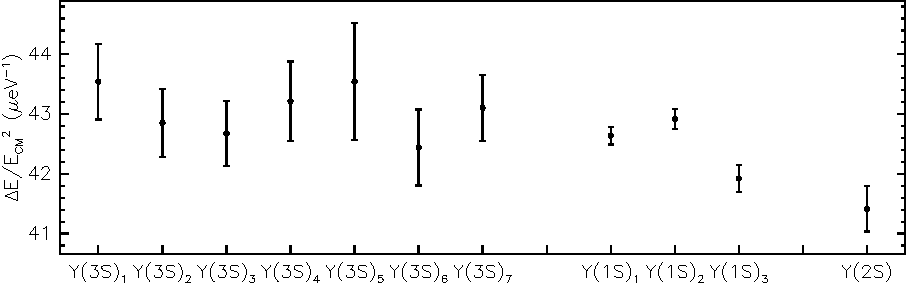
\includegraphics[width=\linewidth]{plots/beamenergyspread}
  \end{center}
  \caption{\label{beamenergyspread} Beam energy spread fit results in
  the center-of-mass ($\Delta E = \sqrt{2}$ single beam energy spread)
  divided by \ecm$^2$, which is nearly constant, as expected.  The
  third \us\ measurement (April 2002) is 2.4\% lower than the second
  (March 2002).}
\end{figure}

The beam-beam interaction region is a ribbon 0.18~mm tall (out of
the ring plane), 0.34~mm wide (in the ring plane but perpendicular to
the beam axis), and 1.8~cm long (in the ring, along the beam axis).
Electrons and positrons may collide anywhere within this constrained
distribution, and its center drifts by about 1--2~mm on a monthly
timescale.  We can easily track these changes.

In addition to \ee\ collisions, beam particles can interact with gas
nuclei inside the beam-pipe and with the wall of the beam-pipe itself
(2.1~cm in radius).  To minimize the number of beam-gas events, the
beam-pipe is kept evacuated at 2--4$\times 10^{-8}$~torr.  Beam-wall
events are minimized by focusing.  The electron and positron currents
can vary independently, so electron-induced beam-gas and beam-wall and
positron-induced beam-gas and beam-wall rates are not identical.  In
fact, we find that positron-induced rates are typically twice
electron-induced rates, suggesting a difference in cross-sections.

We collected eleven independent scans of the \us, totalling
0.27~fb\inv, six \uss\ scans, totalling 0.08~fb\inv, and seven \usss\
scans, totalling~0.22 fb\inv, of which 0.09, 0.05, and 0.08~fb\inv,
respectively, were dedicated exclusively to the lineshape scans.  (The
rest is from the multipurpose samples taken at the resonance peaks.)
The dedicated scan periods were typically ten hours long and spaced by
intervals of a week from late November 2001 through early August 2002.
In addition to scan data, we used the full 0.19, 0.41, and
0.14~fb\inv\ off-resonance datasets, 20~MeV below the \us, \uss, and
\usss\ masses, to subtract continuum backgrounds.

\section{CLEO Detector}

The CLEO detector is a general-purpose assembly of detectors built
concentrically around the CESR interaction point.  This analysis uses
only three of CLEO's detectors: the silicon vertex detector and
central drift chamber for identifying charged tracks, and the CsI
crystal calorimeter for measuring particle energies and for simple
particle identification.  The CLEO-III apparatus, which is the
generation of CLEO in operation in 2001--2002, is depicted in
Figure~\ref{cleoiii}.

\begin{figure}[p]
  \begin{center}
    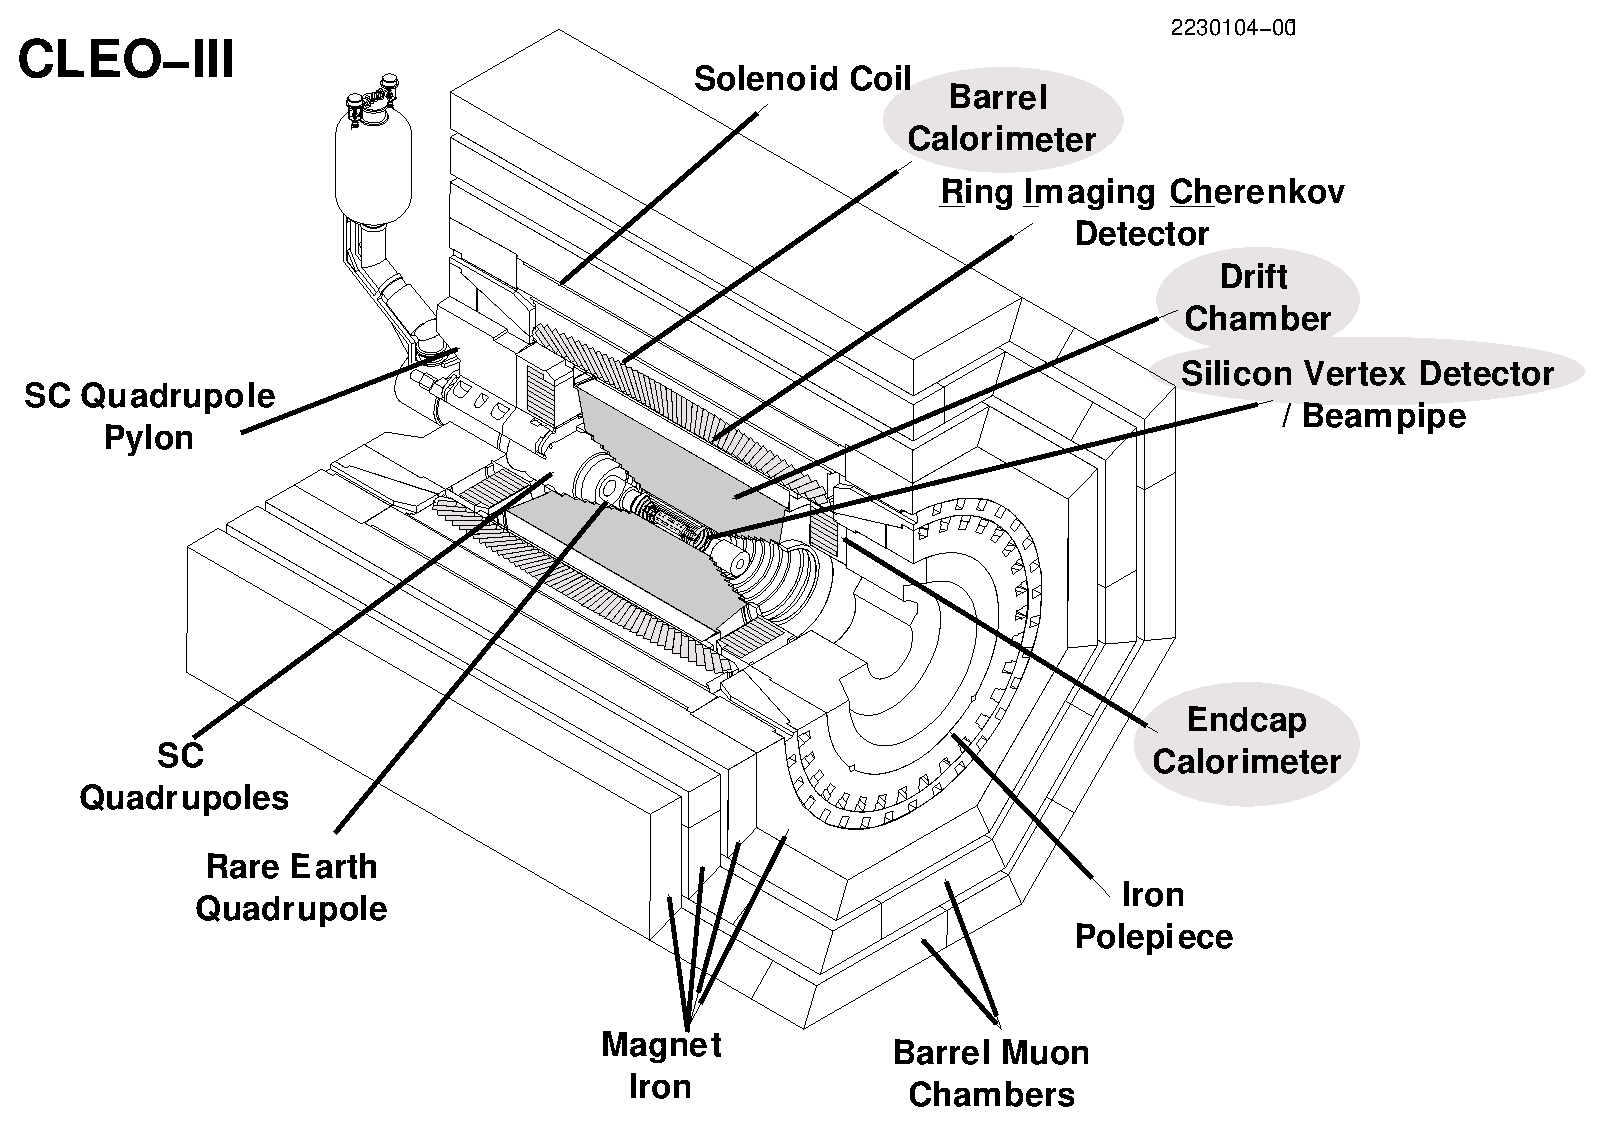
\includegraphics[height=0.8\linewidth, angle=90]{plots/cleoiii}
  \end{center}
  \caption{\label{cleoiii} An isometric view of the CLEO-III detector,
  highlighting the silicon vertex detector, the drift chamber, and the
  CsI crystal calorimeter in gray.}
\end{figure}

We define the $z$ axis of our coordinate system to be parallel with
the beam-line, pointing in the direction of the incident positron
current (west).  Our coordinate system is right-handed, with $y$
pointing up and $x$ pointing away from the center of the CESR ring
(south).  The origin of the coordinate system is within 1--2~mm of the
beam-beam collision point.  This coordinate system is illustrated in
Figure~\ref{coordinatesystem}.  The CLEO detector has an approximate
cylindrical symmetry around $z$, so we also define the polar angle
$\theta$ of a particle trajectory originating at the origin to be the
angle between the trajectory and the beam-line, or $\theta =
\tan^{-1}\left(\sqrt{x^2+y^2}/z\right)$.  We often use $\cos\theta$
and $\cot\theta$ to describe the polar angle, as this centers
trajectories in the $z=0$ plane at zero.  The azimuthal angle $\phi$
is the angle for which $\cos \phi = x/\sqrt{x^2+y^2}$ and $\sin \phi =
y/\sqrt{x^2+y^2}$.

\begin{figure}[p]
  \begin{center}
    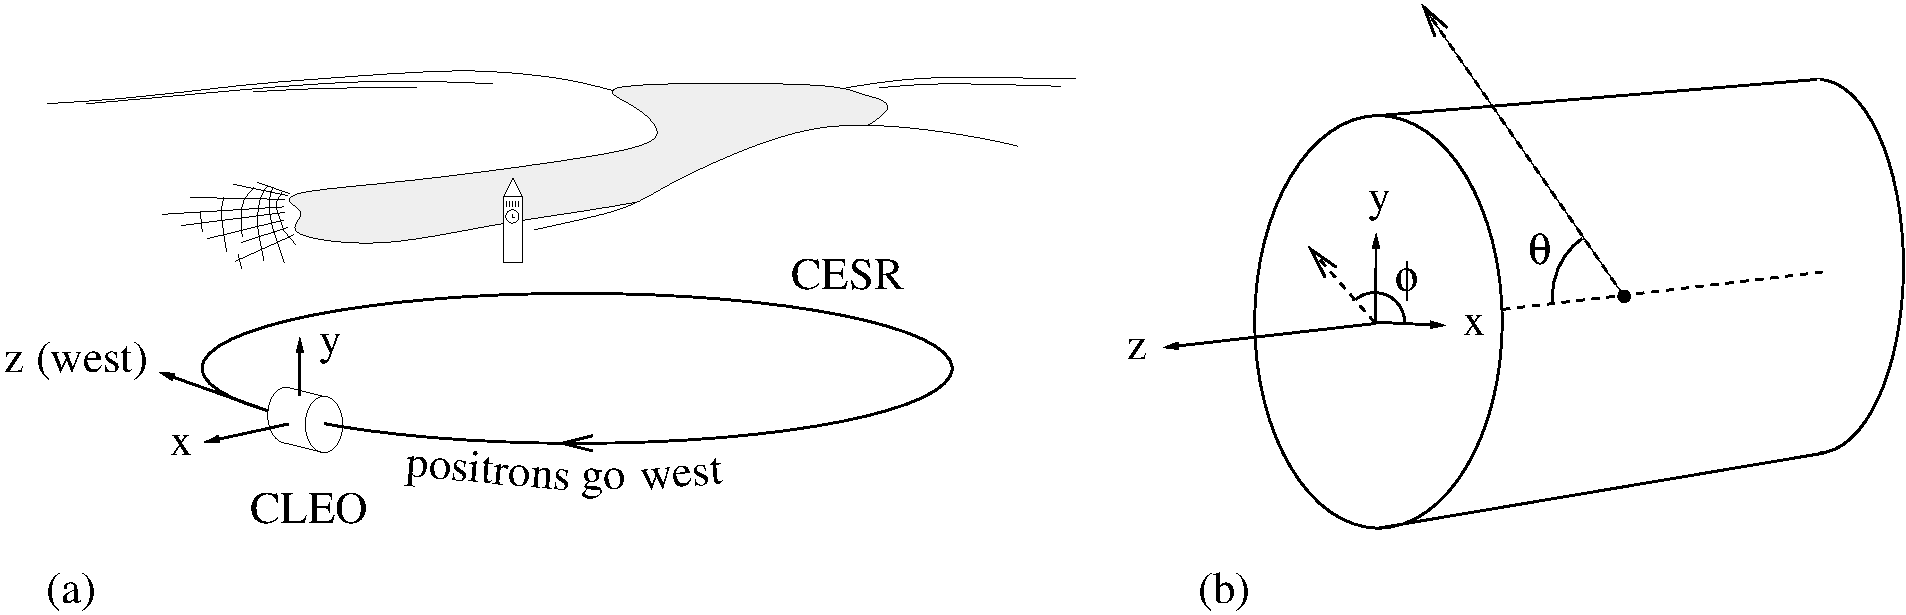
\includegraphics[width=\linewidth]{plots/coordinatesystem}
  \end{center}
  \caption{\label{coordinatesystem} Coordinate system of the CLEO
  detector: (a) orientation with respect to the CESR ring and the
  Earth, (b) definition of $\theta$ and $\phi$.}
\end{figure}

The silicon vertex detector and the drift chamber both detect tracks
by collecting charge left in the wake of ionizing, high-energy
particles.  In the vertex detector, the ionized medium is silicon, cut
into strips held perpendicular to the trajectories of most particles
(Figure~\ref{sidiagram}).  The charge is conducted out of the detector
for amplification along traces which are parallel to the beam-line on
one side of the strip and perpendicular to it on the other, so that
the two-dimensional point of intersection may be reconstructed.

\begin{figure}[p]
  \begin{center}
    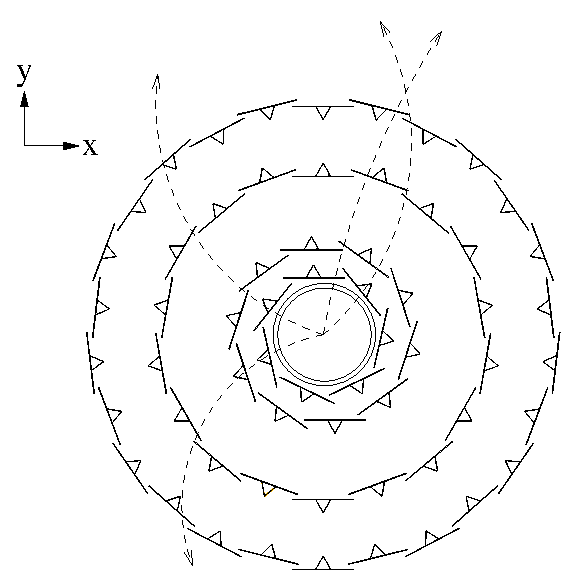
\includegraphics[width=0.5\linewidth]{plots/sidiagram}
  \end{center}
  \caption{\label{sidiagram} Silicon vertex detector geometry,
  projected onto the $x$-$y$ plane.  The trajectories of central
  ($\theta \approx \pi/2$) collision products (dashed lines) are
  roughly perpendicular to the wafers of silicon.  Triangles represent
  diamond rods holding the wafers in place.}
\end{figure}

In the drift chamber, high-energy charged particles ionize a
helium-propane gas (60\% He, 40\% C$_3$H$_8$) in a strong electric
field generated by wires strung across the detector volume, parallel
with the $z$ axis.  This field causes the freed electrons to drift
away from the field wires toward a sense wire strung between them,
which conducts the charge to amplifiers for analysis
(Figure~\ref{driftcell}).  As the electrons drift several millimeters
toward the sense wire, they ionize more atoms, causing an avalanche
that provides a 10$^7$ amplification.  We carefully measure the time
between the first ionization (estimated from bunch collision times)
and charge collection on the sense wire to reconstruct the distance of
closest approach of the high-energy charged particle to the sense
wire, through the known electron drift speed of 28~$\mu$m/ns.  This
technique provides 88~$\mu$m resolution in the $x$-$y$ plane.
Sensitivity to $z$ position is obtained by twisting the outer wires,
presented in more detail in Figure~\ref{stereotwist}.  The outer
31~layers of wires, called the stereo section, are twisted
21--28~mrad, yielding a $z$ position resolution of 3--4~mm at each
wire.  The inner 16~layers, called the axial section, are untwisted.

\begin{figure}[p]
  \begin{center}
    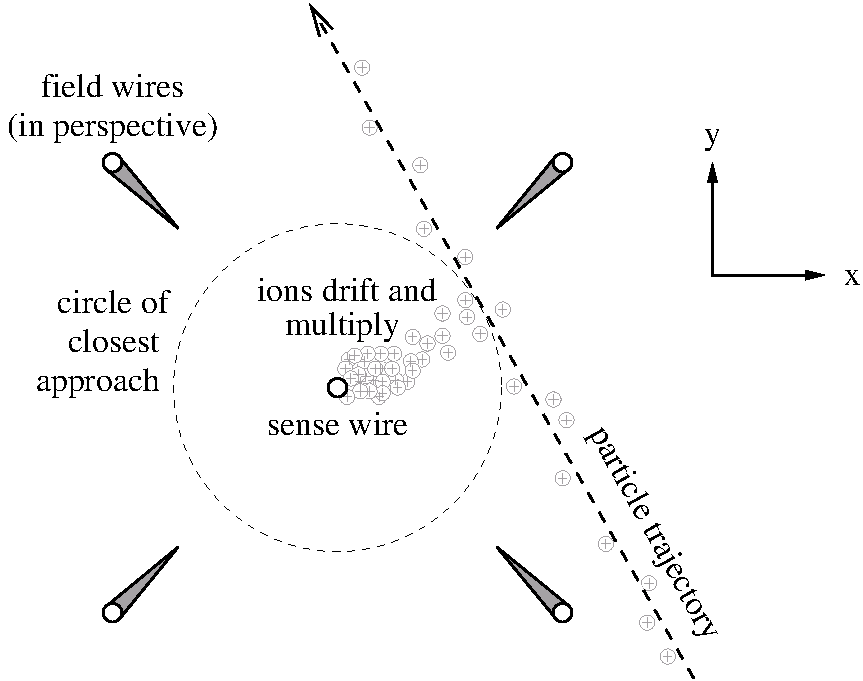
\includegraphics[width=0.65\linewidth]{plots/driftcell}
    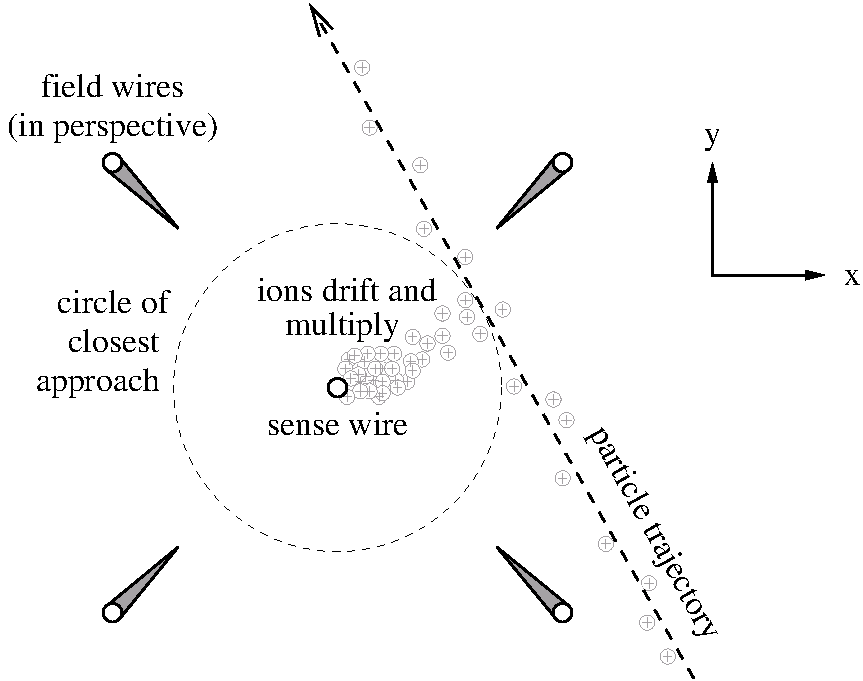
\includegraphics[width=0.6\linewidth]{plots/driftcell}
  \end{center}
  \caption{\label{driftcell} Charge collection and multiplication in
  the drift chamber.  {\it (This Figure needs some work.)}}
\end{figure}

\begin{figure}[p]
  \begin{center}
    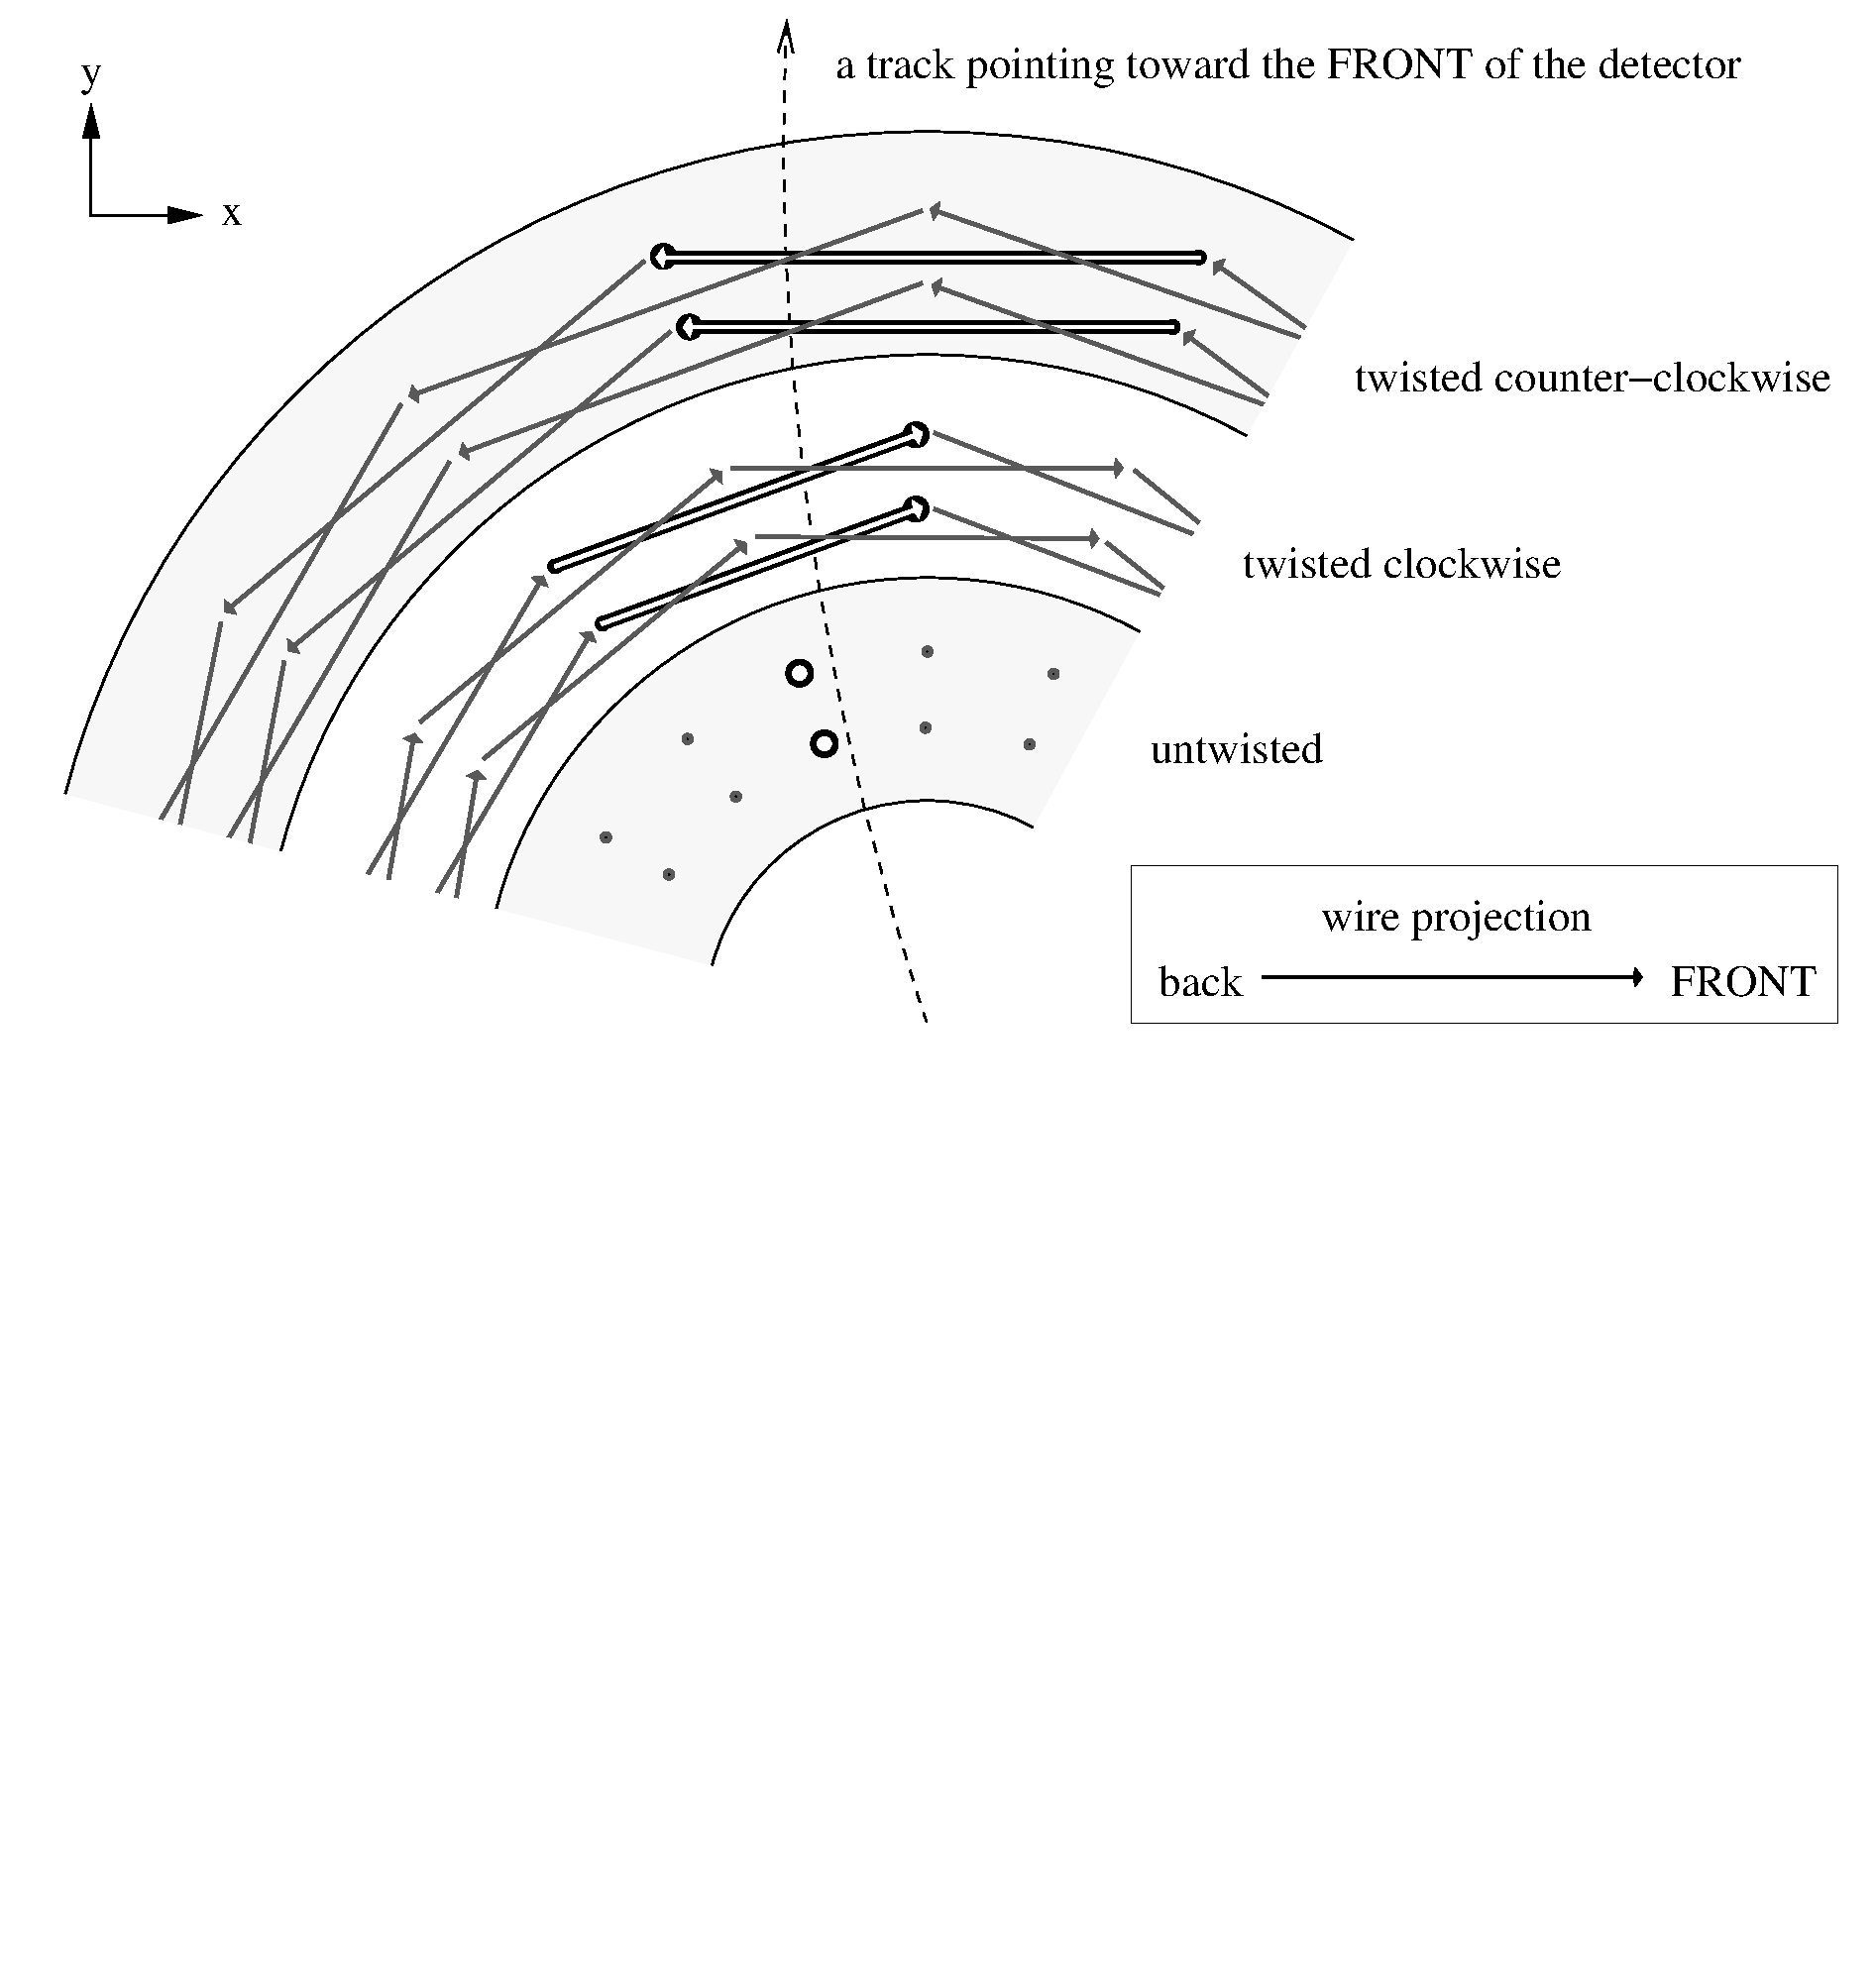
\includegraphics[width=\linewidth, viewport=0 480 892 947]{plots/stereotwist}
  \end{center}
  \caption{\label{stereotwist} Using twisted wires to obtain $z$
  information in the drift chamber.  Twisted wires extrude lines in
  the $x$-$y$ projection; position along a twisted wire indicates the
  $z$ of the track helix near that wire.  The closest wires to the
  track (in three dimensions) are highlighted.}
\end{figure}

Both tracking volumes are permeated by a 1.5~T magnetic field,
pointing along the $z$ axis.  Charged particle trajectories are
helical in this field: projections onto the $x$-$y$ plane are circles.
The polar angle $\theta$ of such a helical trajectory is a constant of
the motion, but not $\phi$.  We measure the charge $\times$ momentum
of particles through the radii of curvature of their tracks.  Only
electrons, muons, pions, kaons, protons, and deuterons are
sufficiently stable and abundantly produced to be observed as tracks,
and all of these particles have $\pm$1 units of charge, so the radius
of curvature provides access to momentum.  The momentum resolution,
dominated by drift chamber measurements, is 0.9\% for beam-energy
tracks, and position resolution near the interaction point, dominated
by silicon vertex measurements, is 40~$\mu$m in $x$-$y$ and 90~$\mu$m
in $z$.

The outer radius of the drift chamber is 80~cm from the interaction
point, and the outer edges are $\pm$110~cm in $z$.  The drift
chamber's $z$ range is more limited for smaller radii to accommodate
the focusing quadrapole magnet, as shown in Figure~\ref{quarterview}.
It will later to useful to know that charged particles with more than
60~MeV of $z$-momentum exit the detector before completing one
half-orbit in the magnetic field.  Such particles cannot generate
multiple tracks by spiralling inside the detector volume.
\label{pag:spiraling}

\begin{figure}[p]
  \begin{center}
    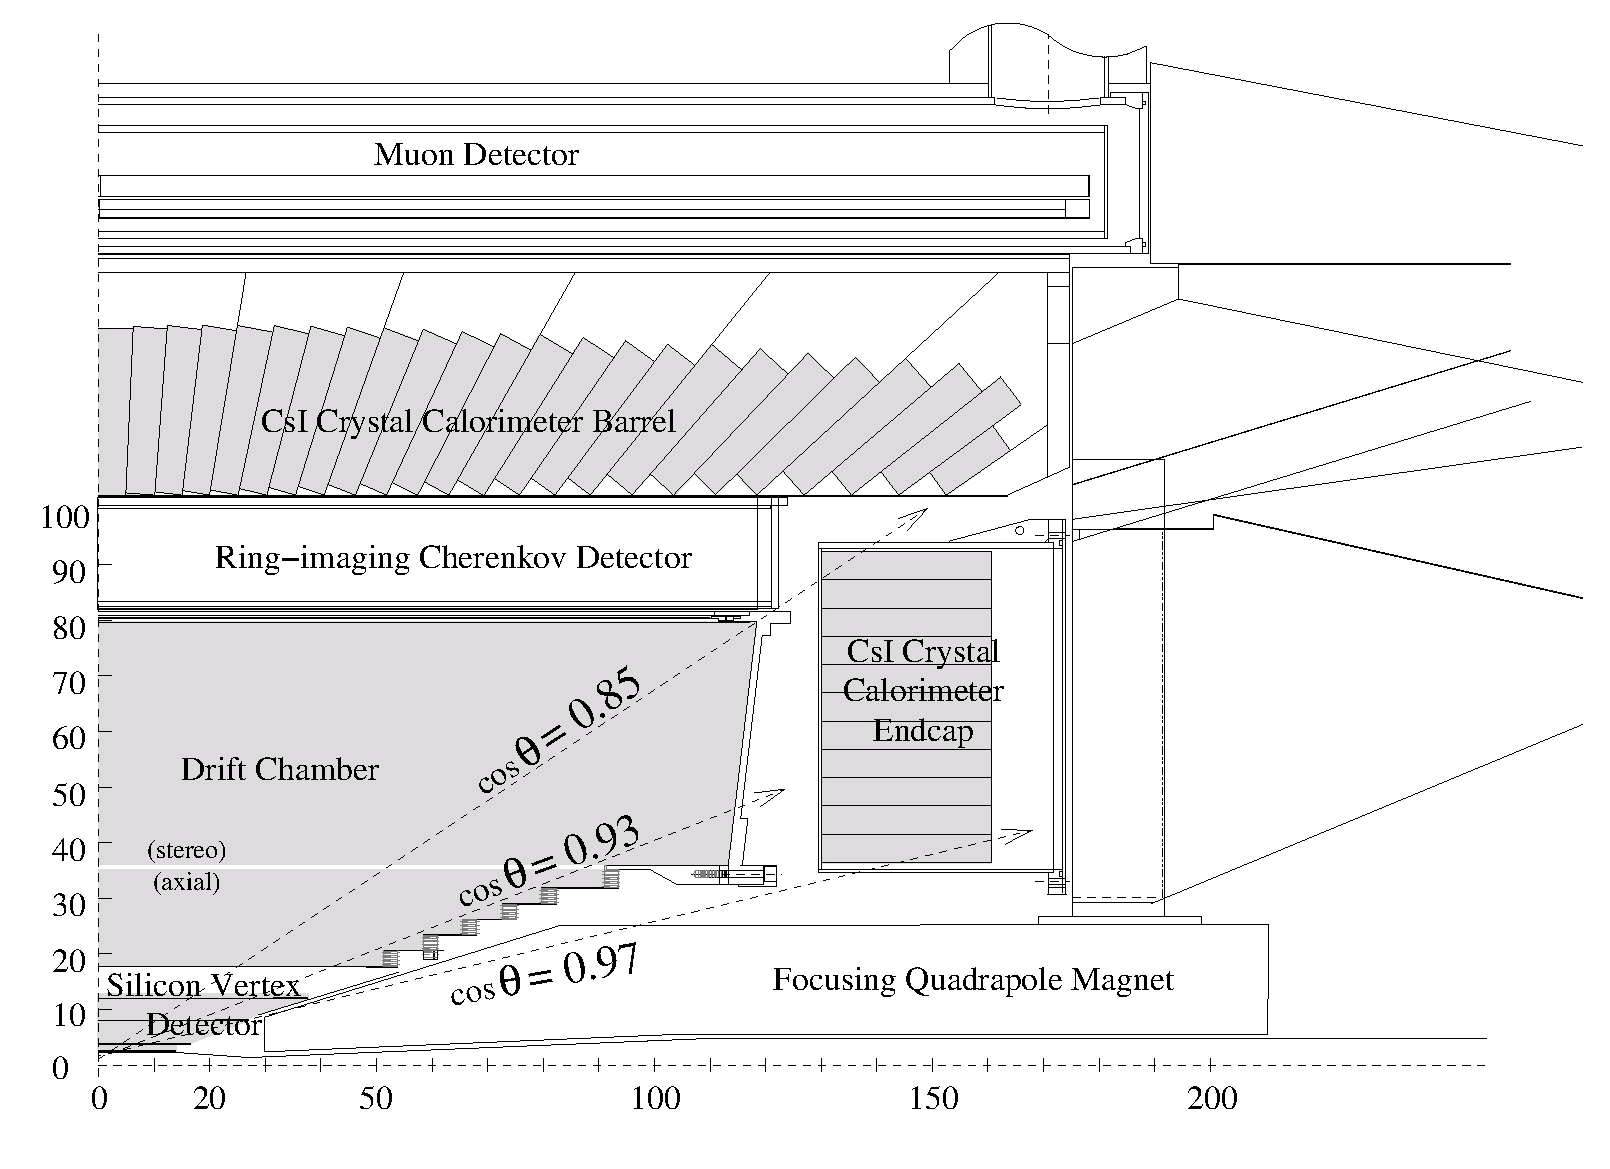
\includegraphics[height=0.8\linewidth, angle=90]{plots/quarterview}
  \end{center}
  \caption{\label{quarterview} A quarter of the CLEO detector,
  highlighting the silicon vertex detector, the drift chamber, and the
  CsI crystal calorimeter in gray.  Radial and $z$ distances are in
  centimeters; the angular reach of the calorimeter barrel, the drift
  chamber, and the calorimeter endcap are illustrated by dashed lines.}
\end{figure}

The CsI crystal calorimeter is sensitive to photons as well as charged
particles, by presenting a transparent, high-$Z$ material for them to
interact with electromagnetically.  (Our thallium-doped CsI has a
radiation length of 1.83~cm.)  The incident particle is destroyed by
this interaction, and replaced by a shower of equal total energy in
less energetic photons, electrons, and positrons.  Visible light from
the shower is collected on the back of the 30~cm-long crystals,
from which the incident energy is reconstructed.  Electrons and
photons with energies near the 5~GeV beam energy are fully
reconstructed with 1.5\% resolution, but muons from typical events
deposit only 200~MeV in the calorimeter, regardless of incident
energy.  Combining the energy of calorimeter showers with track
momenta is sufficient to identify and distinguish \ee, \mumu, and
\gamgam\ events with negligible backgrounds.

The calorimeter geometry is composed of three parts: a barrel
surrounding the tracking volume and two endcaps, beyond the tracking
volume in $z$ (see Figure~\ref{quarterview}).  The calorimeter barrel
covers polar angles with $|\cos\theta| < 0.85$ and the endcaps extend
this range to $|\cos\theta| < 0.97$.  The angular limits of the
tracking volume is between these two: $|\cos\theta| < 0.93$.

When a threshold amount of activity is observed in the drift chamber
and calorimeter, readout electronics are triggered to acquire a
snapshot of the detector and record it as an event.  This activity is
quantified in terms of the number of observed tracks and the number of
showers above given energy thresholds.  For speed, tracks are counted
using a lookup table of drift chamber hits, trained by a simulation,
and showers are approximated by summing calorimeter barrel output over
2$\times$2 tiles, called clusters, and counting the number that
surpass a given threshold.  The number of \axial\ tracks is the number
of tracks reconstructed in the axial section of the drift chamber, and
\stereo\ is the number of tracks which can be extended into the stereo
section.  A \cblo\ cluster exceeds 150~MeV, a \cbmd\ exceeds 750~MeV,
and a \cbhi\ exceeds 1500~MeV.  Real showers can be distributed over
as many as four tiles, sometimes dividing their energy such that none
of the clusters reach a threshold.  This is a source of trigger
inefficiency for final states that rely on shower information
(Figure~\ref{topher}).  After the data have been recorded, we
reconstruct tracks and showers with much finer precision.

\begin{figure}[p]
  \begin{center}
    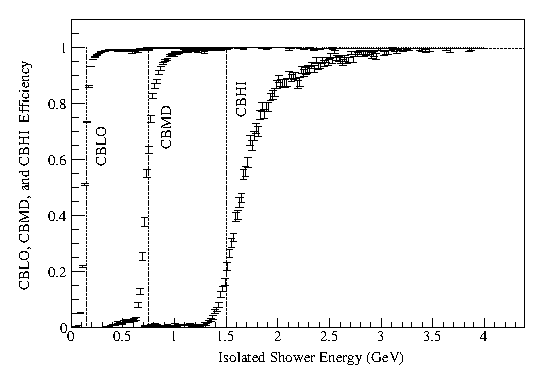
\includegraphics[width=\linewidth]{plots/topher}
  \end{center}
  \caption{\label{topher} The efficiencies of \cblo, \cbmd, and \cbhi\
  identification as a function of fully-reconstructed shower energies
  for isolated showers.  The efficiency curves are not symmetric
  around their thresholds because shower energy may be divided among
  tiles.}
\end{figure}

We use several algorithms to accept events, all of which are
minimum-thresholds: an event is never rejected for having too many
tracks or clusters.  All of these algorithms are active, and when an
event is recorded, it is tagged with the names of the algorithms it
satisfied.  The trigger algorithms relevant for this analysis are
\begin{itemize}

  \item \twotrack, which requires $\ge$2 \axial\ tracks, prescaled by
  a factor of 19 (5.3\%~of the events satisfying this criterion are
  accepted),

  \item \hadron, which requires $\ge$3 \axial\ tracks and $\ge$1 \cblo, \label{pag:triggerdefs}

  \item \radtau, which requires $\ge$2 \stereo\ tracks and ($\ge$1 \cbmd\ or $\ge$2 \cblo),

  \item \eltrack, which requires $\ge$1 \axial\ track and $\ge$1 \cblo, and

  \item \barrelbhabha, which requires 2 \cbhi\ clusters on opposite
  sides of the calorimeter barrel.

\end{itemize}
To count hadronic \ups\ decays, we select only those events which
satisfied \hadron, \radtau, or \eltrack, the three triggers that are
efficient hadronic decays.  (This simplifies our efficiency study.)
Note that a minimal condition for these three trigger algorithms is
that at least one \axial\ track and one \cblo\ were observed.  This
minimal requirement is exact because \stereo\ tracks, being extensions
of \axial\ tracks, are always be less numerous than or equal in number
to \axial\ tracks, and \cbmd\ clusters are also \cblo\ clusters.

Electron and positron beams are circulated in CESR for about an hour
before their currents are exhausted.  Data collected during this time
is called a run, and is given a unique, ascending 6-digit identifier.
Runs are the basic unit of CLEO data samples; in lineshape scans, we
generally took one run at each \ecm\ point at a time.

For some studies, we must simulate our entire detector on a computer.
Such Monte Carlo simulations are most important in determining the
efficiency-corrected cross-section for Bhabhas in CLEO, which is
needed to measure the integrated luminosity of our datasets.  While
the total Bhabha cross-section is infinite, the efficiency-corrected
cross-section, defined by observed Bhabhas, is finite and must be
calculated theoretically.  This calculation has two ingredients, the
differential cross-section as a function of $\theta$ and CLEO's
efficiency for Bhabhas as a function of $\theta$.  The first
ingredient is calculated with perturbative Quantum Electrodynamics
(QED), but the second requires specific knowledge of our detector.
While this efficiency may be approximated as a step function, in which
CLEO observes all Bhabhas within a $\theta$ range and misses all
Bhabhas outside of this range, such a simplification would be bought at a
high price in accuracy.  For the 1\% precision demanded by this
analysis, we must consider all effects: detector geometry, electron
propagation and scattering in materials, sub-component response
efficiency, fringe magnetic fields from the CESR magnets, et cetera.
Our Monte Carlo simulation is based on the GEANT framework, and is
carefully tuned to reproduce the real detector's output at all levels
of analysis.

\chapter{Backgrounds and Event Selection}
\label{chp:backgrounds}

To define a set of hadronic \ups\ decays, we will accept only those
events which satisfy given criteria, or cuts.  We want this set of
events to include as many hadronic \ups\ decays as possible, to
minimize the efficiency correction for lost events.  We therefore only
seek to reduce the backgrounds to a manageable level by cutting out
regions of parameter space where the hadronic \ups\ contribution is
minimal.  We accomplish this with a set of four explicit cuts.

With such an approach, we cannot completely eliminate backgrounds,
especially because continuum \qqbar\ final states are identical to
about 10\% of \ups\ decays.  Instead, we estimate and subtract the
backgrounds which remain after cuts, which we can do very accurately
using control data.  If we can accurately subtract any residual
backgrounds after cuts, why cut at all?  There are two reasons: large
background subtractions introduce large statistical uncertainties, and
the trigger itself selects events in a way which can be hard to
predict, leading to systematic uncertainties.  By imposing more
restrictive event selections with fully-reconstructed data, we can
render the trigger biases insignificant.

\section{Suppressing Backgrounds with Event Selection}

Bhabha scattering is our largest potential background before cuts, and
among our largest backgrounds after cuts.  We suppress Bhabhas by
requiring the largest track momentum, \pmax, to be less than 80\% of
\ebeam.  This rejects a very small fraction of hadronic \ups\ events,
but almost all $\Upsilon \to e^+e^-$ and \mumu\ (Figure~\ref{pmax}).
We do not make a similar requirement on calorimeter shower energy,
which also peaks at \ebeam\ for each electron in the Bhabha event,
because we find track momentum measurements to be more stable in time
than shower energy measurements.  Unlike track momentum, which is a
geometric measurement of wires in space, shower energy depends
sensitively on the amplification of the calorimeter read-out.  This
amplification is measured with 0.02--0.06\% precision, but the Bhabha
spectrum is so steep that \bork\% of Bhabha showers move across a
reasonable threshold (75\% of \ebeam) with these fluctuations in
energy scale.

\begin{figure}[p]
  \begin{center}
    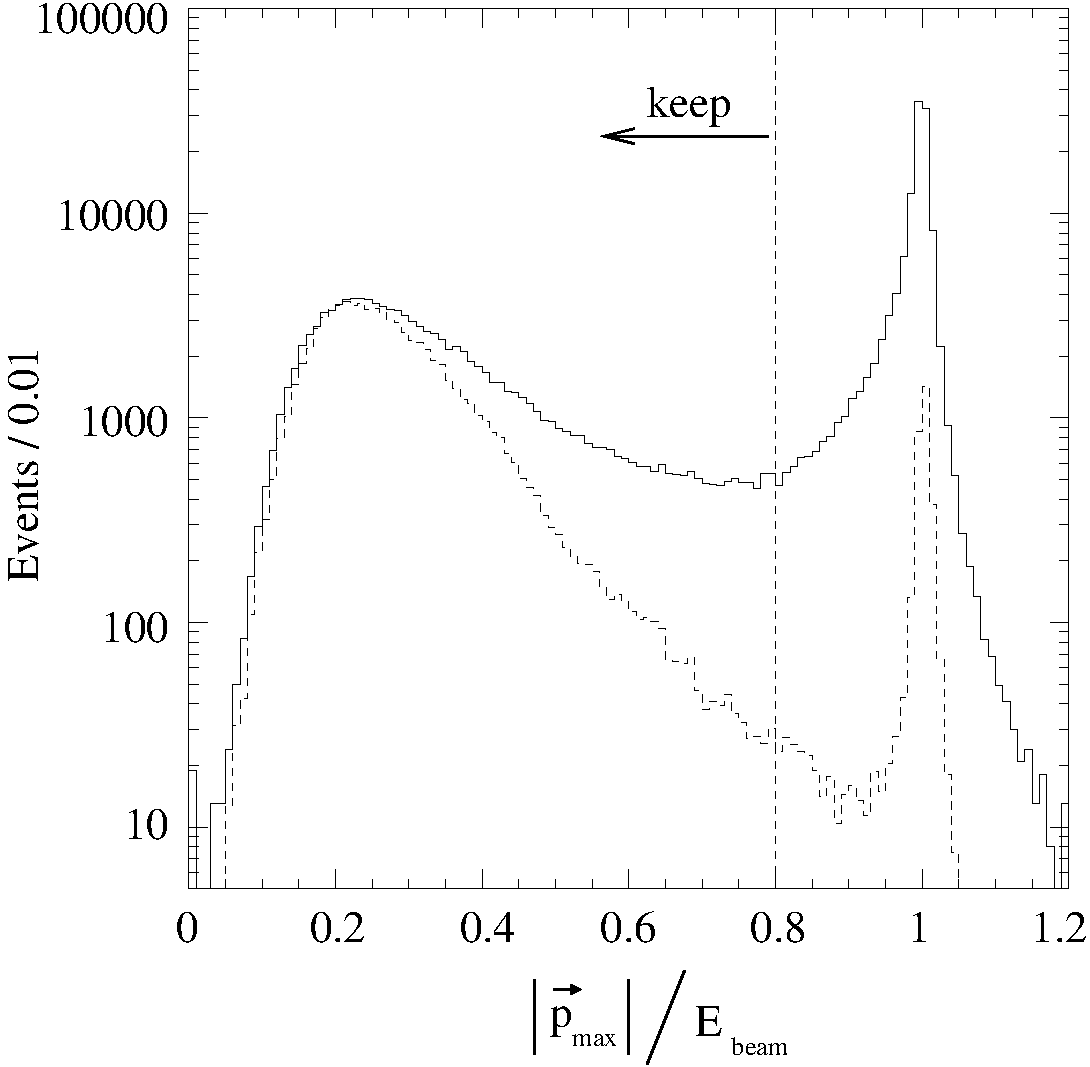
\includegraphics[width=\linewidth]{plots/pmax}
  \end{center}
  \caption{\label{pmax} Largest track momentum (\pmax) in each event
  for data (solid histogram) and Monte Carlo \ups\ decays (dashed),
  with all other cuts applied.  Data have large backgrounds from
  Bhabhas and radiative Bhabhas.  Hadronic \ups\ decays peak at 20\%
  of \ebeam, while $\Upsilon \to e^+e^-$ and \mumu\ peak at 100\% of
  \ebeam.}
\end{figure}

It is also common to reject Bhabhas by requiring more than two tracks
in the event: most hadronic events have more than two tracks and
Bhabhas should have exactly two.  We considered this cut at an early
stage in the analysis, but decided against it because we found the
number of tracks distribution difficult to simulate for hadronic
events.  At that time, we intended to determine the cut efficiency
with a Monte Carlo simulation, so this would have contributed
significantly to our systematic uncertainty.  Since then, we have
found a way to measure hadronic efficiency without resorting to
simulations, but we did not re-introduce the cut because we do not
need it.  The \pmax\ cut reduces Bhabha contamination to approximately
the same level as continuum \qqbar, so the Bhabha contribution to the
statistical uncertainty of the background-subtracted count is not
dominant.  (Several of our cuts imply that an event must generate at
least one track, but this does not significantly affect the Bhabha
background.)

As previously mentioned, the cross-section of all continuum $e^+e^-
\to f\bar{f}$ processes ($f$ is any fermion) fall off as $1/s$ while
two-photon fusion events ($e^+e^- \to e^+e^- X$) increase as $\log s$.
Continuum $f\bar{f}$ may therefore be estimated and subtracted
collectively, while two-photon fusion must be handled separately,
possibly introducing systematic error if it is large.  We therefore
suppress two-photon fusion events by requiring the visible energy of
the event, \visen, to be greater than 40\% of \ecm.  Visible energy is
the sum of all track energies (determined from momentum, assuming the
charged particle to have a mass of 140~MeV) and neutral shower
energies (neutral showers must be at least 7~cm from all tracks).  If
all particles in an event are detected, \visen\ $\approx$ \ecm.  As
seen in Figure~\ref{visen}, hadronic \ups\ events peak in \visen\ at
80\% \ecm, and there is a peak of non-\ups\ events at 15\% \ecm.  At
least two-thirds of the events in this low-\visen\ peak are two-photon
collisions, in which one incident electron has taken most of the
center-of-mass energy, undetected, down the beam-pipe.  We know this
because two-thirds of events with \bork--\bork\% visible energy
contain one low-momentum electron, whose charge and direction are
correlated with the incident beams, and a highly anisotropic
distribution of shower energy, presumably from the boosted hadron
system $X$.  Decays of \tautau\ cover a broad spectrum of \visen, due
to energy lost in one or two neutrinos, extending but not peaking
below our cut threshold.

\begin{figure}[p]
  \begin{center}
    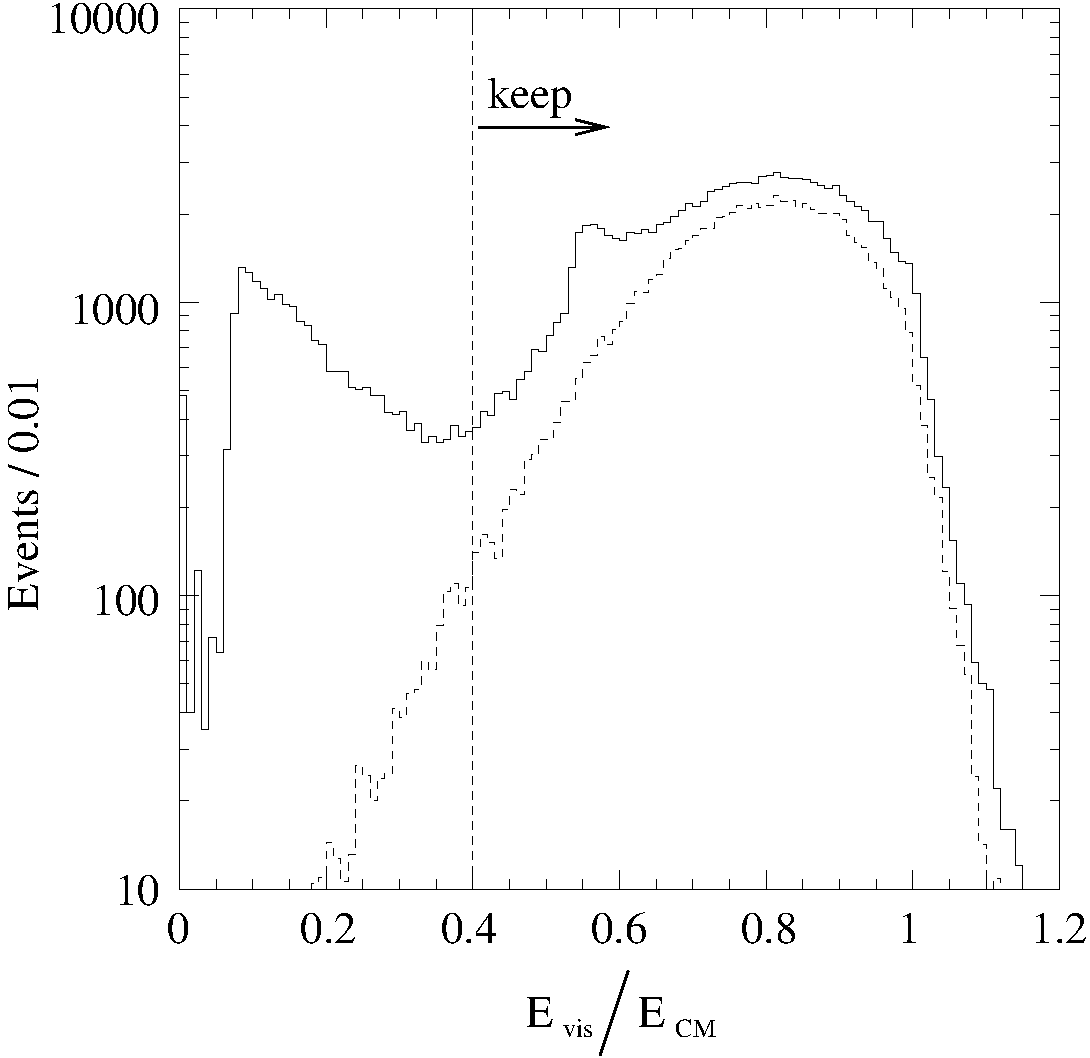
\includegraphics[width=\linewidth]{plots/visen}
  \end{center}
  \caption{\label{visen} Total visible energy (\visen) in each event
  for data (solid histogram) and Monte Carlo \ups\ decays (dashed)
  with all other cuts applied.  At least two-thirds of the peak at
  15\% of \ecm\ in data are two-photon fusion events, and the peak
  above 50\% of \ecm\ are likely to be radiative Bhabhas, missing an
  electron.  See text for a more complete discussion.}
\end{figure}

Rejecting low-\visen\ events also protects our hadron count from
uncertainties associated with trigger thresholds.  Only about 0.1\% of
hadronic events with \visen\ $>$ 40\% \ecm\ fail to trigger, so any
fluctuations in the electronics will be on this level.  The \visen\
threshold, situated in the flat minimum between the two-photon peak
and the signal peak, is minimally sensitive to fluctuations in the
two-photon background and the signal efficiency.  According to Monte
Carlo, only 0.8\% of the hadronic \ups\ decays fail this cut, so any
fluctuations in this efficiency will be well under a percent.

In addition to the two-photon peak at an \visen\ of 20\% \ecm, there
is an excess of events with \visen\ just above 50\% \ecm\ (Figure~\ref{visen}).  These events are likely to be radiative Bhabhas
($e^+e^- \to \gamma e^+e^-$) in which one of the two electrons is
lost.  They contain neutral calorimeter energy and an energetic
electron whose charge and direction is correlated with the incident
beams, like the two-photon fusion events.  However, visible energy in
two-photon collisions is expected to be much less than 50\% of \ecm.

The number of background events from a continuum process is
proportional to the integrated luminosity, just like the number of
signal \ups\ decays.  Their contribution to the apparent cross-section
will therefore be purely a function of \ecm.  The same cannot be said
for backgrounds that are not the product of beam-beam collisions.
Beam-gas and beam-wall rates are a function of the individual beam
currents, the gas pressure inside the beam-pipe (for beam-gas) and the
extreme tails of the bunch shape (for beam-wall).  Cosmic rays are
abundant in our detector, and the number of cosmic ray events is only
a function of time.  Integrated luminosity, current-time, and time are
approximately proportional (within a factor of two), so a continuum
subtraction largely removes these effects, but not entirely.

We suppress beam-gas, beam-wall, and cosmic ray events by requiring
the event to originate near the beam-beam crossing point.  To select
events originating near this point in an $x$-$y$ projection, we
require at least one track to extrapolate within 5~mm of the beam-line.
We define \dxy\ as the distance of closest approach of the closest
track to the beam-line, and reject events with \dxy\ $>$ 5~mm.  Tracks
extrapolated from the tracking volume are corrected for momentum loss
in the beam-pipe and silicon detector, and the location of the
beam-beam crossing point is measured independently for each run, using
the first 500 hadronic events.  The \dxy\ distribution
(Figure~\ref{dxy}) is much narrower than our 5~mm threshold: only
0.1\% of beam-beam collision events fail this cut.  This allows for
$\sim$1~mm errors in the beam-beam intersection measurement, which is
far larger than the expectation.

\begin{figure}[p]
  \begin{center}
    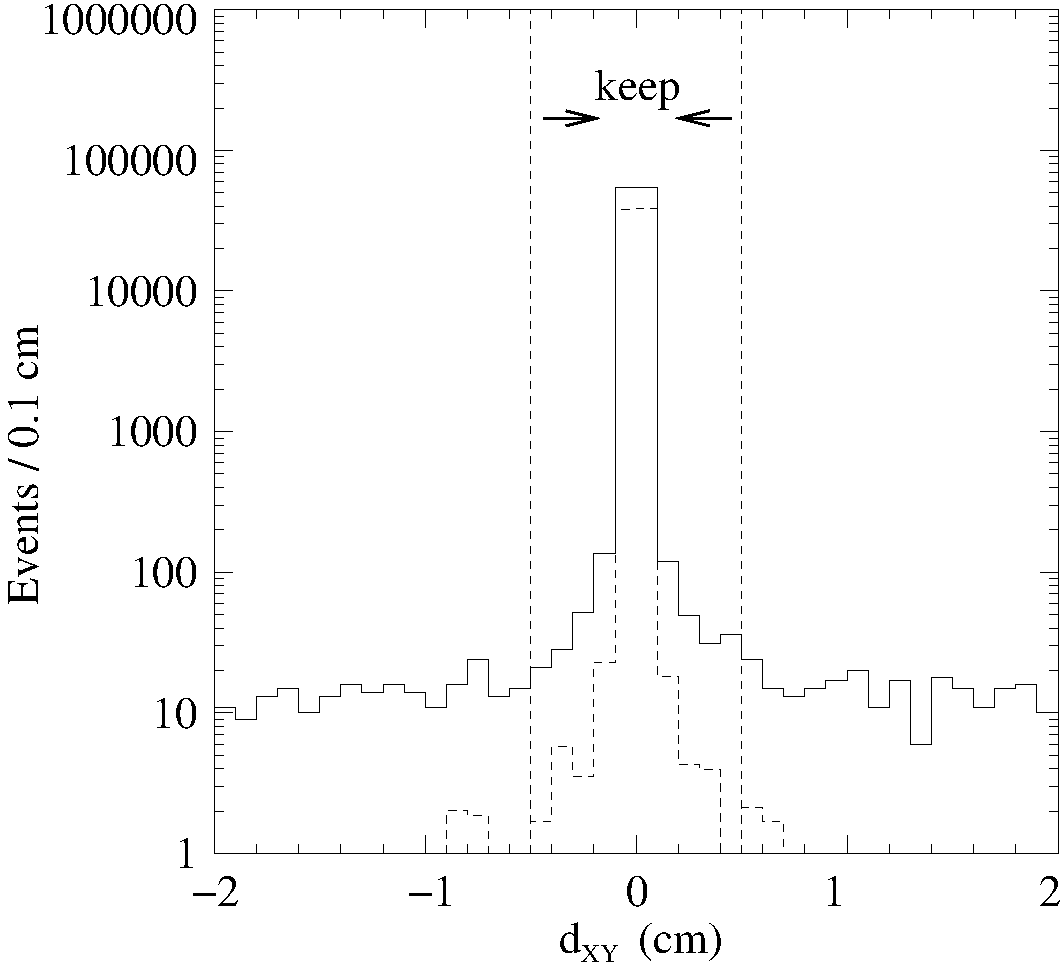
\includegraphics[width=\linewidth]{plots/dxy}
  \end{center}
  \caption{\label{dxy} Distance from the closest track projection to
  the beam-line for data (solid histogram) and Monte Carlo \ups\ decays
  (dashed) with all other cuts applied.  The sign is related to the
  orientation of the track's curvature.  The flat background in data
  is due to cosmic rays.}
\end{figure}

Our \dxy\ cut is extremely effective at rejecting cosmic ray events.
Cosmic rays rain uniformly onto the detector, generating a uniform
background to \dxy, which extends to 40~cm with our triggers.  Only
those cosmic rays that pass within 5~mm of the beam-line survive.  In
principle, beam-wall events should also be eliminated, since they are
generated in the beam-pipe, 2~cm from the beam-line.  However, beam-wall
events contain several tracks, any one of which may project into the
accepted \dxy\ region (Figure~\ref{biastowardzero}).  By selecting
events using the closest track, we bias this background to peak within
our accepted region, diluting the effectiveness of the cut.

\begin{figure}[t]
  \begin{center}
    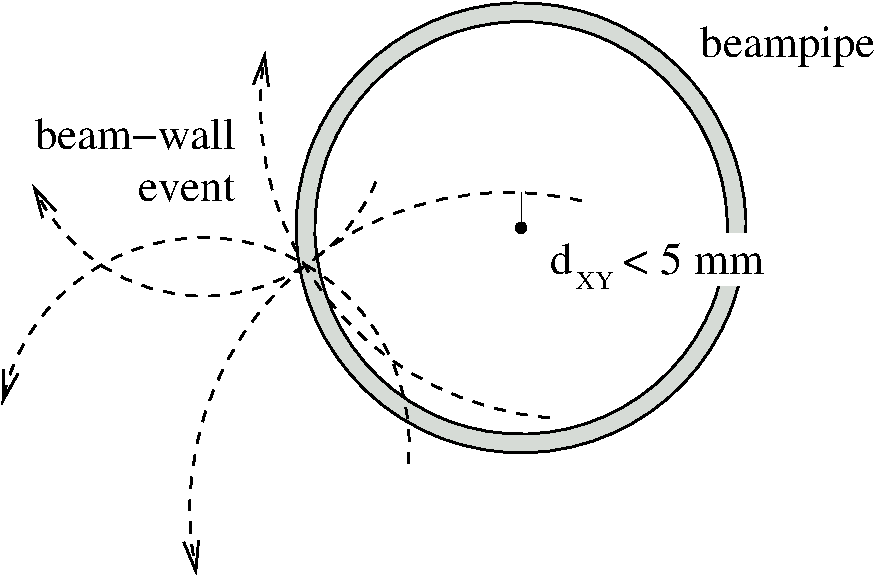
\includegraphics[width=0.6\linewidth]{plots/biastowardzero}
  \end{center}
  \caption{\label{biastowardzero} Though beam-wall events are centered
  at the beam-pipe, tracks may still project within 5~mm of the
  beam-line, thus passing the \dxy\ cut.}
\end{figure}

Beam-gas and beam-wall events originate along the beam-line and
beam-pipe, extending beyond beam-beam collisions in $z$.  Placing a
requirement on the closest track to the $z$-collision point would be
ineffective for the same reason as above; beam-gas and beam-wall
events both have many tracks, and the probability that one of these
would project into the signal region (which is several centimeters
wide) is roughly a half.  Instead, we reconstruct the $z$ position of
the event vertex using all tracks, and call this quantity \dz.  The
CLEO event vertexing algorithm is not useful because it was designed
for signal reconstruction and fails to fit too many of our messy
beam-gas and beam-wall events.  Instead, we developed a simple
algorithm of our own.  Tracking resolution is such that most of the
tracks from a beam-beam collision intersect within 0.1~mm of a common
origin in the $x$-$y$ plane, and the number of intersections near this
point grows rapidly with the number of primary tracks.  Accidental
track intersections far from this point grow more slowly.  We can
therefore determine the event vertex very accurately by averaging the
$z$ positions of track-track intersections.  We define the $z$
position of an $x$-$y$ intersection to be halfway between the $z$
positions of the two track helices, evaluated at the $x$-$y$
intersection point.  If the intersection is a true three-dimensional
vertex, the tracks' $z$ positions will be nearly equal.  We weight
these intersections with uncertainties propagated from the track
uncertainties, the tracks' $z$ separation, and the $x$-$y$ distance to
the beam-line added in quadrature, to prefer true intersections from
the primary vertex.  We plot this \dz\ distribution in Figure~\ref{dz}, and cut very loosely at 7.5~cm, to allow for errors in the
beam-beam intersection measurement.

\begin{figure}[p]
  \begin{center}
    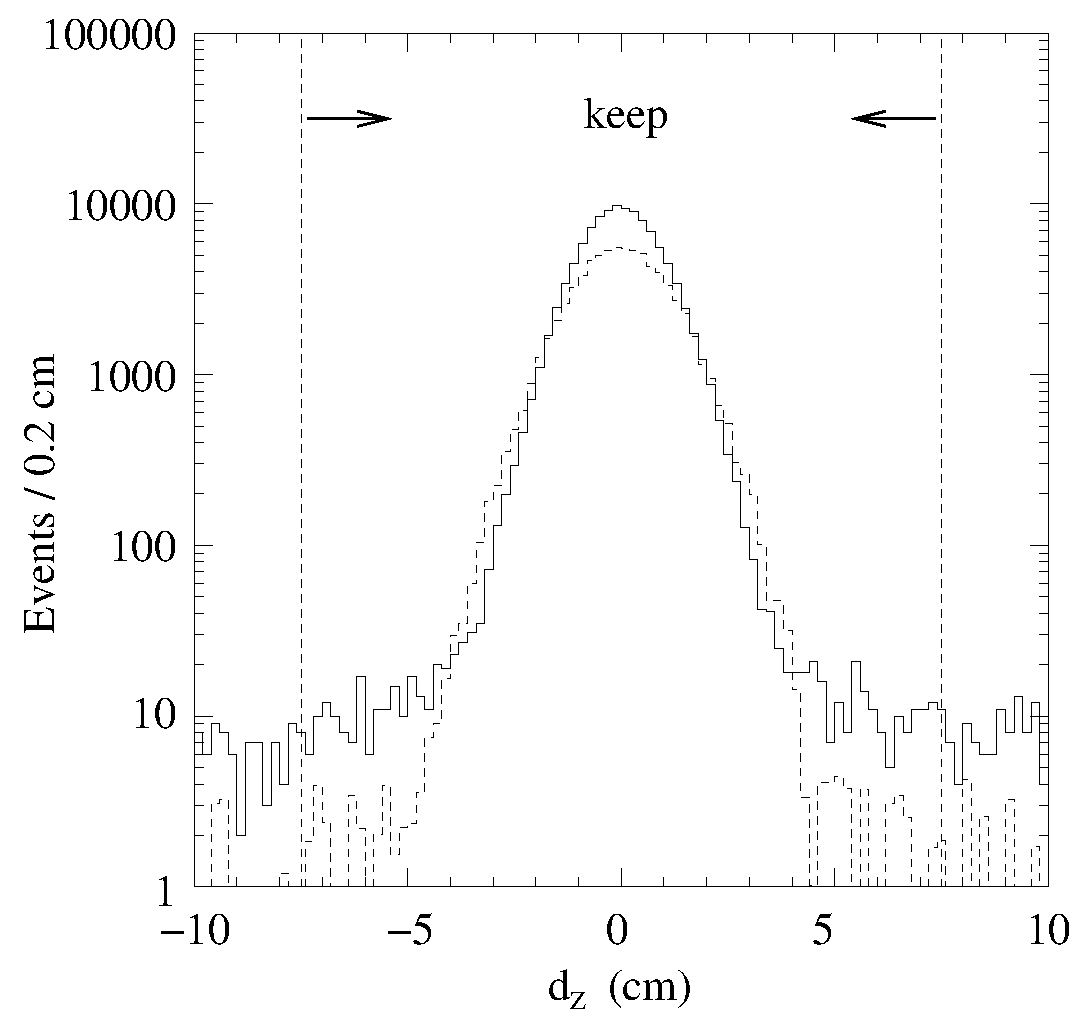
\includegraphics[width=\linewidth]{plots/dz}
  \end{center}
  \caption{\label{dz} Location of the event vertex in $z$, according
  to our algorithm, for data (solid histogram) and Monte Carlo \ups\
  decays (dashed) with all other cuts applied.  Data and Monte Carlo
  differ in the $z$-length of the beam-beam overlap region.  The flat
  background in data is primarily beam-gas and beam-wall, though Monte
  Carlo indicates that 0.5\% of \ups\ decays are misreconstructed and
  extend beyond the cut threshold.}
\end{figure}

We can also use track intersections to distinguish beam-wall events
from beam-gas.  The distance of the closest track-track intersection
to the beam-line will be nearly zero for beam-gas events, but peak
below the beam-pipe radius of 2.1~cm for beam-wall events (because
selecting the closest intersection to the beam-line biases the
distribution toward zero).  In Figure~\ref{smallbeamwall}, we plot the
distribution of closest intersections for events with \dxy\ $<$ 5~mm
from data with only one beam in CESR.  We see that the \dxy\ cut
reduces beam-wall to the extent that it is approximately as common as
beam-gas.  A more sophisticated average of intersections could help to
discriminate between beam-gas and beam-wall, but as we will see in
Subsection~\ref{sec:bgbwcr}, these two processes combined are a small
contamination, about 0.2\% of the continuum for most runs.

\begin{figure}[p]
  \begin{center}
    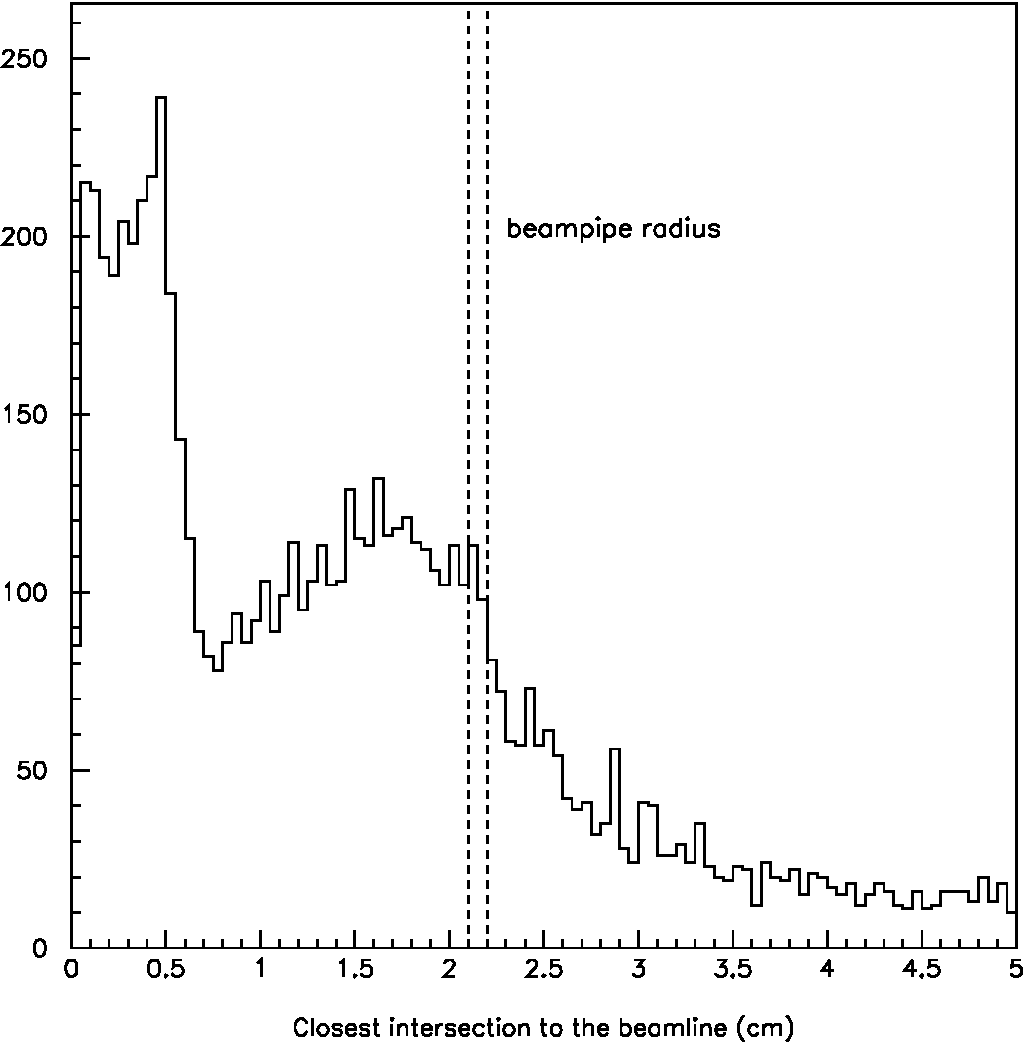
\includegraphics[width=\linewidth]{plots/smallbeamwall}
  \end{center}
  \caption{\label{smallbeamwall} Closest track-track intersection to
  the beam-line in special data with one, non-colliding beam in CESR
  (all events are beam-gas, beam-wall, and cosmic rays).  The rough
  peak below 0.6~cm is mostly beam-gas, and the broad peak from 1 to
  2~cm is due to beam-wall events.}
\end{figure}

\section{Data Quality Requirements}
\label{sec:quality}

Not all data were collected under ideal conditions, so we applied some
general criteria for rejecting bad runs.  As the data were collected,
two CLEO operators inspected the data for hardware failure.  In the
most serious cases, these data were eliminated from all CLEO analyses,
but if the effect was limited, it was listed in a ``bad runs'' file
({\tt /home/dlk/Luminosity/badruns3S}).  We rejected any runs that
were flagged with drift chamber, silicon vertex detector, or CsI
calorimeter problems.

We want a robust measurement of cross-section, and cross-section is
constant with time, even as the beam currents are depleted during a
run.  We therefore checked for variations in cross-section during each
run by comparing hadronic events and \gamgam\ events in hundredths of
each run.  This ratio fluctuates statistically, but we found two
examples in which the drift chamber lost sensitivity to tracks before
the calorimeter lost sensitivity to showers in the last few minutes of
the run (Figure~\ref{crashruns}).  Most likely, the drift chamber lost
high voltage just before the end of the run.

\begin{figure}[p]
  \begin{center}
    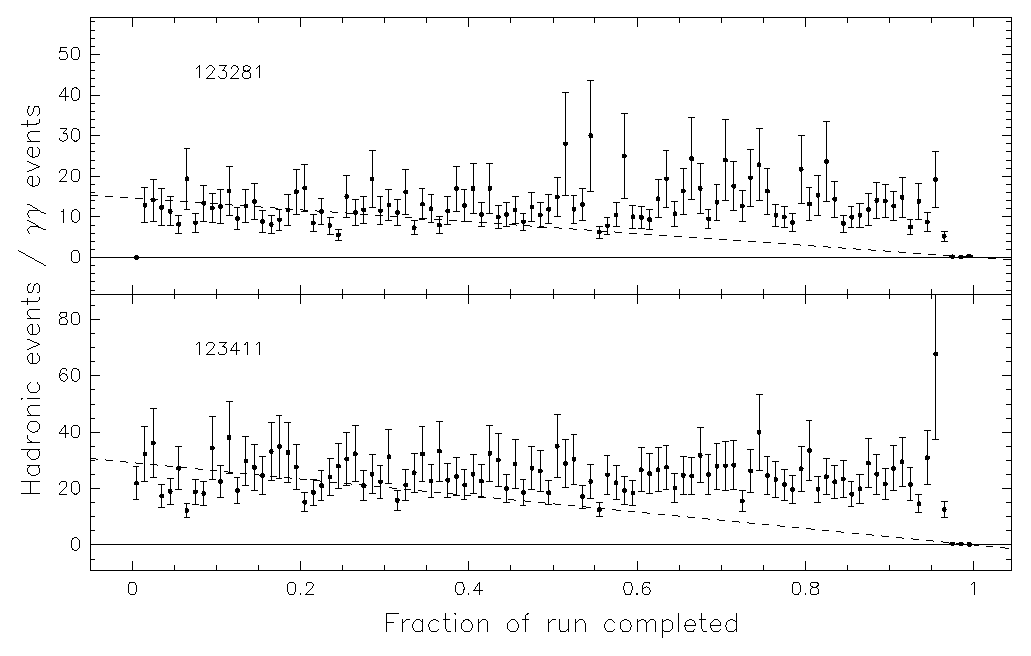
\includegraphics[width=\linewidth]{plots/crashruns}
  \end{center}
  \caption{\label{crashruns} Ratio of hadronic events to \gamgam\
  events as a function of time through two runs.  The hadronic
  cross-section drops to zero in the last 3\% of these runs (the
  dashed lines are linear fits to the data.)}
\end{figure}

To catch more instances of this kind of failure, we also compared the
rate of trackless Bhabhas to total Bhabhas.  We recognize the \ee\
final state by the two beam-energy showers it produces in the
calorimeter, curved 0.1 radians away from perfect collinearity by the
magnetic field.  Twenty-five runs had high trackless Bhabha rates
(above 0.3\%), and all of the trackless Bhabha excesses were in the
same hundredth of a run (usually the last).  Ten of these (presented
in Figure~\ref{crashruns2}) were crucial to the \ups\ scans and not
rejected.  Instead, we determined the cross-section from the
first 99\% of these runs.  The twenty-seven runs with drift chamber
failures are listed in Table~\ref{tab:runfailures}.

\begin{figure}[p]
  \begin{center}
    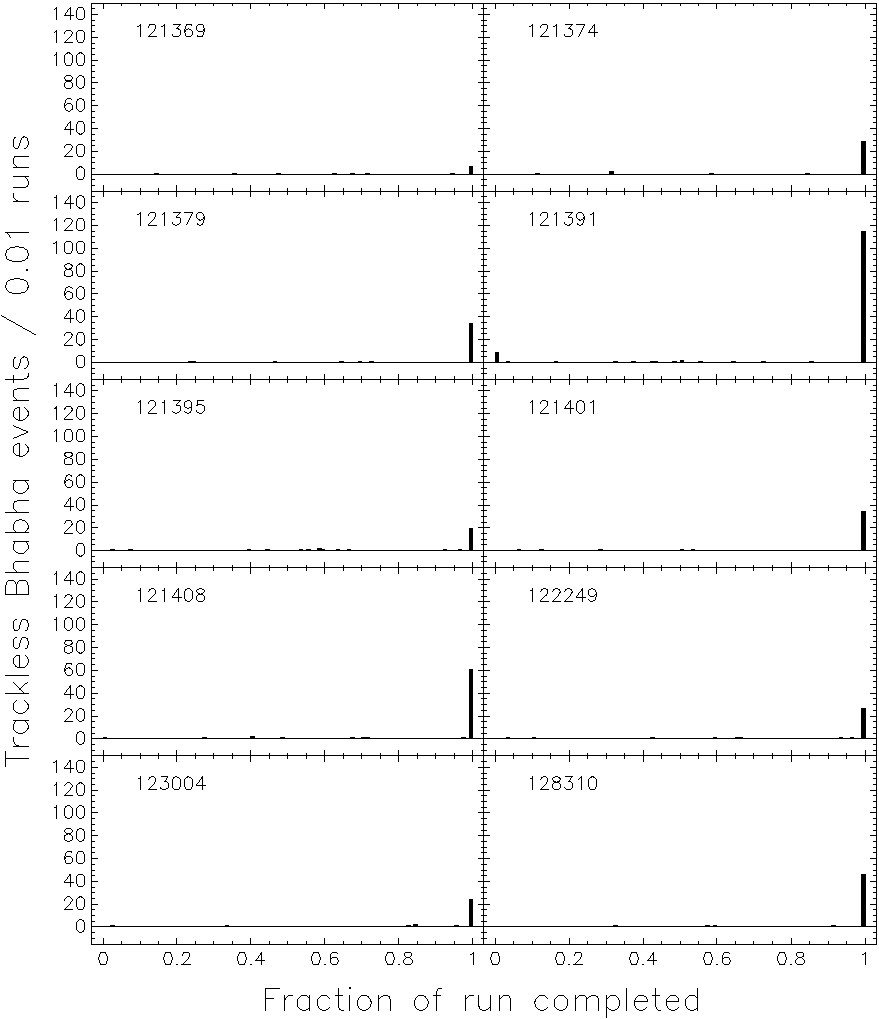
\includegraphics[width=0.95\linewidth]{plots/crashruns2}
  \end{center}
  \caption{\label{crashruns2} Bhabha events with no observed tracks as
  a function of time through ten runs.  In all of these cases, there
  is an excess in the last 1\% of the run.}
\end{figure}

\begin{table}
  \caption{\label{tab:runfailures} Runs rejected for hardware reasons.}
  \begin{center}
    \begin{tabular}{p{0.5\linewidth} p{0.4\linewidth}}
      \hline\hline
      Drift chamber failed at the end of the run & 121476, 121748, 121822, 121847, 122685, 123281, 123411, 123436, 123847, 123873, 124816, 124860, 124862, 125367, 126273, 126329, 127280 \\
      \barrelbhabha\ trigger inefficiency & 121928, 121929, 121953, 127951, 127955, 130278, 121710, 121930, 121944, 121954, 123884 \\
      Poor track momentum resolution & 124452, 124454, 124456, 124458, 124462, 124464, 124465, 124466, 124467, 124469, 124472, 124473, 124474, 124475, 124477, 124478, 124479, 124480 \\
      Noisy showers in the calorimeter endcap & 122331, 122335, 122336, 122339, 122341, 122342, 122344, 122345, 122349, 122350, 122352 \\
%      Large cosmic ray/beam-gas backgrounds & 122353 (12\% cosmic rays), 126341 (2\% $e^+$ beam-gas), 129522 (2\% $e^+$ beam-gas) \\
      Large cosmic ray/beam-gas backgrounds & 122353, 126341, 129522 \\
      Large, unidentified backgrounds & 121595, 122093, 122330, 126510 \\
      Too little data for tests & 123013, 123014 \\\hline\hline
    \end{tabular}
  \end{center}
\end{table}

The \gamgam\ final state, which we use for some diagnostic checks, is
accepted only by a specialized \barrelbhabha\ trigger.  We studied the
efficiency of this trigger with Bhabha events and discovered eleven
runs with very low efficiency, which we rejected.  These failures
would only have affected our cross-checks.

We also tested the quality of the drift chamber and calorimeter output
by observing the rate of unphysically high-energy tracks and showers.
In good data, only a small fraction of Bhabhas will have tracks and
showers with momenta and energies above 120\% \ebeam.  In a contiguous
block of data on date-\bork, the track momentum resolution tripled
(\borky) abruptly, increasing the rate of unphysical track momenta.
On a separate occasion (date-\bork), one quarter of the calorimeter
endcap exaggerated Bhabha shower energies by a factor of 1.5--2.  We
rejected runs that suffered from either of these malfunctions.

We rejected a handful of runs due to high background rates.  From
Figure~\ref{backgroundsvsrun}, we set a 5\% upper limit on acceptable
cosmic ray yields relative to the continuum yield, and an upper limit
of 2\% on beam-gas.  Three runs failed these criteria.  We also
noticed that the fractions of hadronic, Bhabha, \gamgam, and \mumu\
events dropped abruptly in the middles of four runs, indicating a
sudden turn-on of some large background.  We rejected these, too.
Finally, two runs had so little data (\bork\ events total) that it was
difficult to perform any of the above tests.  We rejected them for
simplicity.

This analysis combines small ``scan'' datasets, taken on the \ups\
resonances but not at its maximum, with off-resonance and ``peak''
data taken at the maximum \ups\ cross-sections.  The scan data were
acquired specifically for this analysis and therefore were not
rejected lightly.  (None of the runs in Table~\ref{tab:runfailures}
are scan runs.)  The peak data is less valuable, and even after the
selections described above, far more is available than is necessary.
A measurement of the area of an \ups\ lineshape (i.e.\ \gee) can be
conceptually decomposed into width measurements and height
measurements, in which the fractional uncertainty in the area is the
sum of the fractional uncertainty in the width and in the height, in
quadrature.  Scan data constrain both the width and the height, while
peak data constrain only the height.  Adding peak data to a fit will
always reduce the statistical uncertainty, though this reaches an
asymptotic limit as the uncertainty comes to be dominated by the width
measurements.  However, as the beam energy calibration drifts with
time, cross-sections slightly off the peak of the resonance may be
represented as being exactly on-resonance, thereby biasing the height
measurement.  We accepted no more peak data than what is necessary to
bring the statistical uncertainties within \bork\% of their limiting
values.  Since we are concerned with potential drifts with time, we
re-expressed this limit as a time limit: we only include peak data in
a lineshape fit if this data were taken less than 48 hours after the
beginning of a scan.  We imposed no such limit on off-resonance data.

We rejected a \us\ scan, acquired on April 3, 2002.  This scan is
missing key cross-section measurements on the high-energy side of the
peak (Figure~\ref{apr03scan}), which makes it difficult to assess
uncertainties in the beam energy and the beam energy spread.  This
scan does include cross-section measurements well above the \ups\
mass, and may have been the victim of miscommunicated beam energy
requests.  (Requests are made relative to the \ups\ mass, and
single-beam energies used by CESR differ from our center-of-mass
energies by a factor of two.)  Its exclusion from the \us\ fit changes
that fit result by \bork\% with no appreciable difference in
uncertainty, because it is also a low-luminosity scan.

\begin{figure}[t]
  \begin{center}
    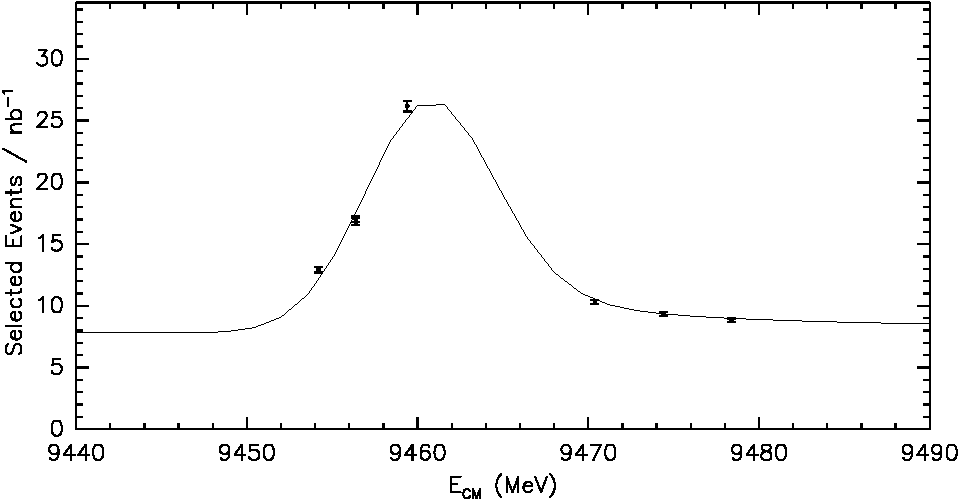
\includegraphics[width=0.8\linewidth]{plots/apr03scan}
  \end{center}
  \caption{\label{apr03scan} The April~3, 2002 lineshape scan,
  overlaid by a fit to all other \us\ scans.  No data significantly
  constrain the high-energy side of the peak.}
\end{figure}

\section{Subtracting Residual Backgrounds}

Backgrounds remaining after our cuts are summarized in Figure~\ref{awesome}.  We will discuss each of these, and their subtractions,
in the subsections that follow.

\begin{figure}[p]
  \begin{center}
    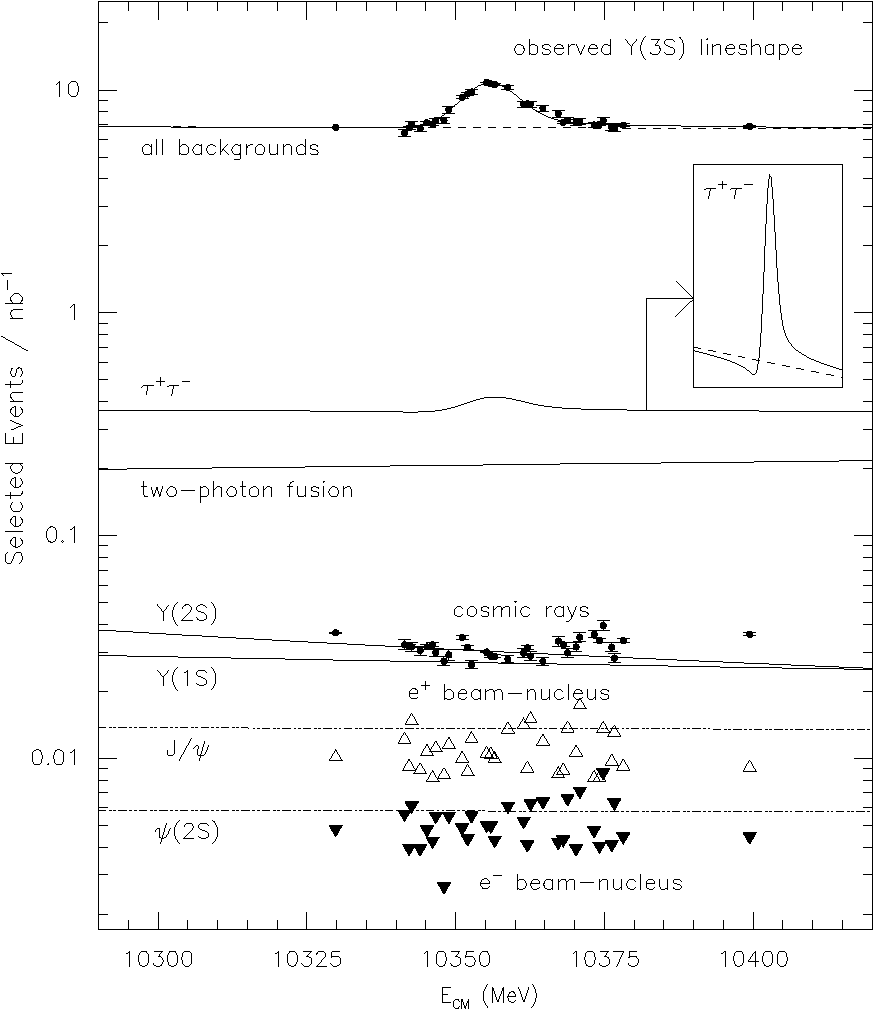
\includegraphics[width=\linewidth]{plots/awesome}
  \end{center}
  \caption{\label{awesome} The \usss\ lineshape in log scale, to
  illustrate backgrounds.  The top dashed curve represents the sum of
  all backgrounds, which is dominated by $1/s$ continuum processes.
  The solid curves and data points below this are non-$1/s$
  corrections included in ``all backgrounds.''  Dashed curves
  represent ISR tails from charmonium resonances which are included in
  the two-photon fusion curve.  The overlap of ISR tail curves and
  non-beam-beam counts is accidental.}
\end{figure}

\subsection{Backgrounds that Vary Slowly with Beam Energy}
\label{sec:varyslowly}

After our cuts, radiative Bhabhas and continuum \qqbar\ dominate the
background, adding a flat, 8~nb mesa below our three \ups\ peaks
(18~nb, 7~nb, and 4~nb, respectively) in apparent cross-section versus
\ecm.  These and all continuum processes except for two-photon fusion
evolve as $1/s$, so we include such a function in our lineshape fits.
The magnitude of this term is determined independently for the \us,
\uss, and \usss\ by the large off-resonance samples taken only 20~MeV
below each \ups\ mass.  The $1/s$ curve is the dashed line near the top
of Figure~\ref{awesome}.

We must apply two corrections to the $1/s$ curve: initial state
radiation (ISR) to lower-energy \ups\ resonances have a $1/(\sqrt{s} -
M_\Upsilon)$ distribution and two-photon fusion grows as $\log s$.
The magnitude of an \ups\ ISR tail is set by the magnitude of the
\ups\ resonance.  We therefore fit \us, \uss, and \usss\ in ascending
order to obtain tail corrections from the previous fits.  The \us\ and
\uss\ ISR tails under the \usss\ peak are labeled in Figure~\ref{awesome}, and Figure~\ref{logsfit} shows \uss\ and \usss\
off-resonance cross-sections with and without this tail correction.

\begin{figure}[p]
  \begin{center}
    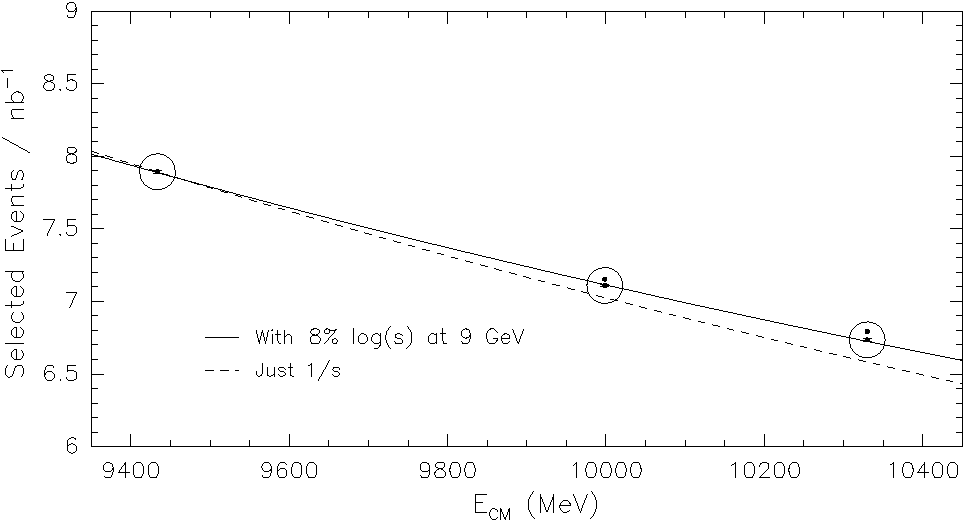
\includegraphics[width=\linewidth]{plots/logsfit}
  \end{center}
  \caption{\label{logsfit} Off-resonance cross-section measurements
  versus \ecm, with and without ISR tail corrections.  (Corrected data
  are at the centers of the circles.)  The solid curve is the best fit
  to $A/s+B\log s$, and the dashed curve is $1/s$ only, constrained to
  pass through the first data point.}
\end{figure}

\label{pag:logs}
To parameterize the $\log s$ correction for residual two-photon
fusion, we fit the three off-resonance cross-sections to $A/s + B\log
s$.  Even after accounting for the ISR tail contribution, we see a
non-$1/s$ component whose apparent cross-section grows with \ecm: the
difference in lineshapes is plotted in Figure~\ref{logsfit}.
According to the fit, this increase is explained if 8\% of the
apparent cross-section at 9~GeV is due to two-photon fusion events.
We can estimate the residual two-photon background after cuts by
extrapolating the low-\visen\ peak above the 40\% of \ecm\ threshold,
plotted in Figure~\ref{extrapolatevisen}.  This extrapolation yields a
two-photon fraction of 6\%, which is roughly consistent with our fit
result.  Other effects may contribute to the $\log s$ term, such as
cut efficiency for continuum events, a slow variation in the hadronic
continuum cross-section, and ISR tails from charmonium resonances
($J/\psi$ and $\psi'$).  All of these effects vary slowly with \ecm,
so our parameterization for large differences in \ecm\ (900~MeV from
\us\ to \usss\ off-resonance) applies to small differences in \ecm\ as
we project the \us, \uss, and \usss\ off-resonance cross-sections
below each peak.  The difference in cross-section between a pure $1/s$
curve and the fully parameterized curve is only 0.04\% at the peak.

\begin{figure}[p]
  \begin{center}
    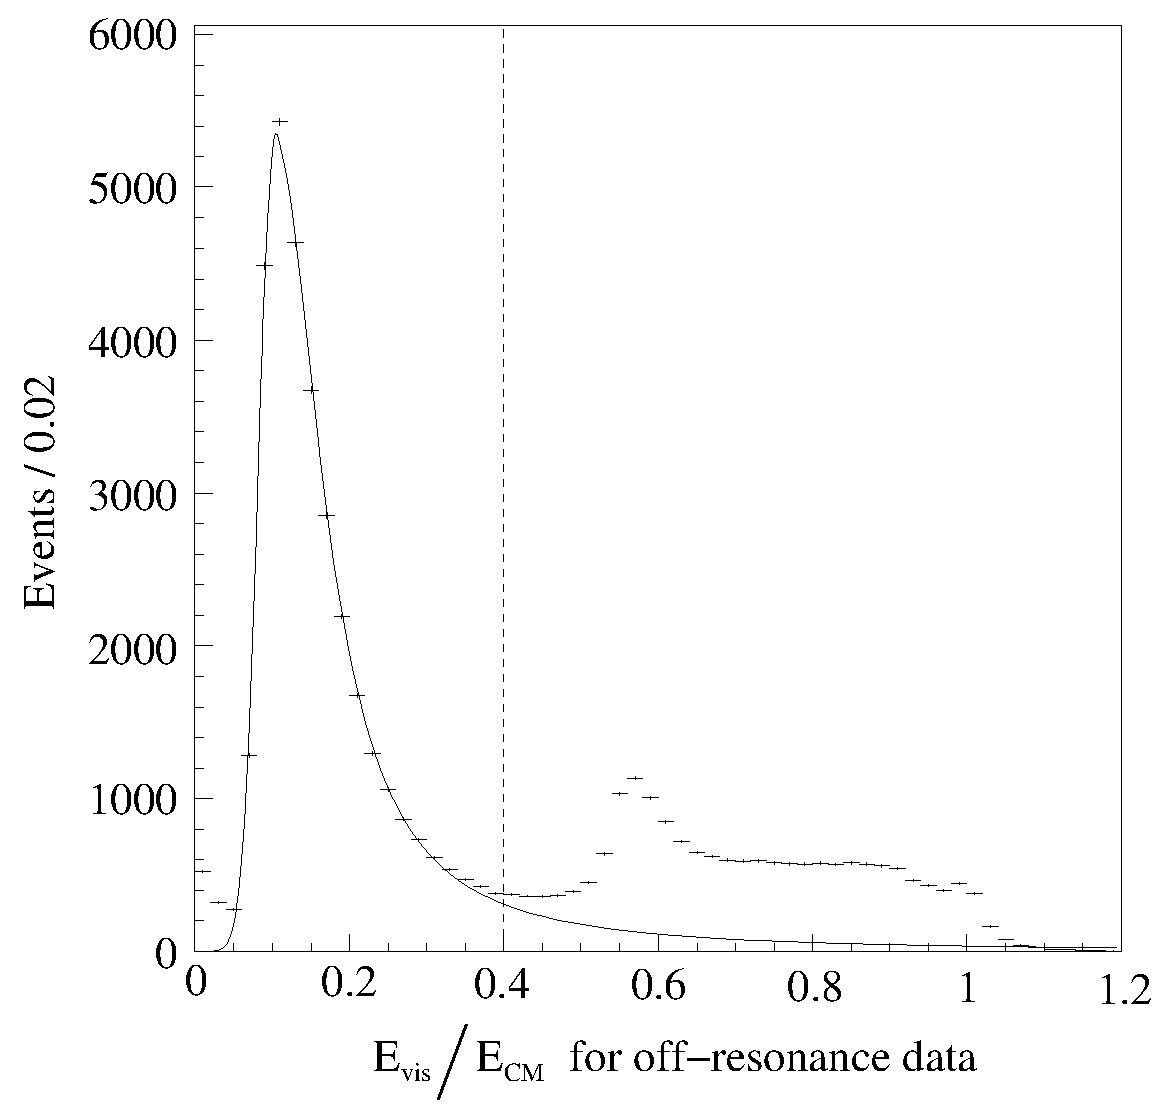
\includegraphics[width=\linewidth]{plots/extrapolatevisen}
  \end{center}
  \caption{\label{extrapolatevisen} The visible energy (\visen) of
  off-resonance data, overlaid with a fit to the low-\visen\ peak.
  The fit is Gaussian on the low-energy side and Lorentzian on the
  high-energy side, and is used to roughly estimate the two-photon
  fusion events which survive after the 40\% of \ecm\ cut (dashed
  vertical line).} % If[x<0.10277, 53098.*Exp[-(x-0.10277)^2/2./0.00041188], 53098.*0.074022^2/((x-0.10277)^2 + 0.074022^2)]
\end{figure}

\subsection{Continuum-Resonance Interference}

As discussed in Section \ref{sec:earlyinterference}, resonant
$\Upsilon \to q\bar{q}$ interferes with continuum \qqbar.  We
must therefore also add a $\tilde{\sigma}_\subs{int}(E_\subs{CM})$ term our
fit function with magnitude $\alpha_\subs{int}$ = \bork\ (see Equation
\ref{eqn:yint}).  This contribution differs from the pure continuum
terms in that $\tilde{\sigma}_\subs{int}(E_\subs{CM})$ is added to
$\sigma_\subs{res}(E_\subs{CM})$ before the two are convoluted by the
beam energy spread and initial state radiation.  Leaving pure
continuum contributions out of the resolution smearing is justified by
the fact that they vary slowly with respect to the 4~MeV beam energy
spread.

In this analysis, we assume that $e^+e^- \to q\bar{q} \to$ hadrons
interferes with $e^+e^- \to \Upsilon \to q\bar{q} \to$ hadrons but not
$e^+e^- \to \Upsilon \to ggg \to$ hadrons, though the latter may share
some final states which are indistinguishable from \qqbar\ decays.
(Interference from \gggamma\ is negligible because its branching
fraction is only 3\% of \ggg\ and most \gggamma\ events have a
distinctive high-energy photon.)  For interference between \qqbar\ and
\ggg\ decays, quantum states must remain coherent through the
hadronization process.  This effect has been observed in $J/\psi$ and
$\psi' \to \pi^+\pi^-$ and $K^+K^-$, but it is unclear if the effect
is significant when summed over all final state amplitudes, which can
cancel.  The phase difference between \qqbar\ and \ggg\ for the
inclusive process is also unknown, and some phases cannot be
constrained by our lineshape fits.  We will therefore only assume
parton-level interference, and discuss hadronic interference as a
fitting issue in Chapter \ref{chp:fitting}.

\subsection{Backgrounds from \boldmath \ups}

Since we are selecting hadronic \ups\ events, $\Upsilon \to e^+e^-$,
\mumu, and \tautau\ are backgrounds which peak under the hadronic
\ups\ signal.  We have no control sample for leptonic \ups\ modes, so
we estimate these with a Monte Carlo simulation: negligible \ee\ and
\mumu\ survive the \pmax\ cut (\bork\ and \bork\%), even with final
state radiation ($\Upsilon \to \gamma e^+e^-$ and $\gamma \mu^+\mu^-$)
modeled by PHOTOS.  Our cuts and trigger are 57\% efficient for
\tautau, however.  A tau lepton may decay into several hadrons, making
it difficult to distinguish from hadronic \ups\ decays.  Tau-pairs are
rejected primarily by the \visen\ cut, as their visible energy
spectrum is very broad due to neutrinos in the final state.

We will need to subtract \tautau\ events from the hadronic \ups\
count.  The \ecm\ dependence of $\Upsilon \to \tau^+\tau^-$ is the
same as $\Upsilon \to$ hadronic, though the magnitudes of the resonant
and interference terms both differ.  The resonant \tautau\
contribution is a factor of ${\mathcal B}_{\tau\tau}/{\mathcal
B}_\subs{had}$ times smaller than the hadonic resonance, and the
\tautau\ interference term has a $\alpha_\subs{int}$ of \bork.  Continuum
\tautau, like continuum \qqbar, are included in the $1/s$ term.  When
we estimate systematic uncertainties in the lineshape parameterization
in Chapter \ref{chp:fitting}, we will note that the uncertainty in
\btt\ overwhelms the uncertainty in \tautau\ efficiency.

\subsection{Beam-Gas, Beam-Wall, and Cosmic Rays}
\label{sec:bgbwcr}

The non-beam-beam backgrounds are not a strict function of integrated
luminosity, so we will need to explicitly subtract them from the
hadronic \ups\ count for each run.  To do this, we identify cosmic ray
events, beam-gas, and beam-wall events in every run with special cuts.
We then use control samples containing only cosmic rays or cosmic
rays, beam-gas, and beam-wall to determine how to relate the number of
non-beam-beam backgrounds that we counted to the number that survive
our hadronic cuts.  We then subtract this excess.

To identify cosmic rays, we require the following.
\begin{itemize}

  \item No track may project within 5~mm of the beamspot (\dxy\ $>$
    5~mm).

  \item The event must contain at least two tracks, since our track
    reconstruction algorithm identifies the descending-radius part of
    the cosmic ray as one track and the ascending-radius part as
    another.

  \item The normalized dot product of the two largest track momenta
    ($\vec{p}_1 \cdot \vec{p}_2 / |\vec{p}_1| |\vec{p}_2|$) must be
    less than -0.999 or greater than 0.999, since the angles of these
    two tracks differ only due to tracking resolution (though the
    orientation may be confused by hits with unexpected drift times).

  \item The total calorimeter energy must be less than 2~GeV,
    consistent with two minimally-ionizing muon showers,

  \item and \visen\ $>$ 4\% of \ecm\ for less sensitivity to trigger
    thresholds.

\end{itemize}
These cuts are, by design, much more efficient for cosmic rays than
our hadronic cuts, but the number of identified cosmic rays and the
number of cosmic rays contaminating our hadron count is proportional.
To determine this constant of proportionality, we apply both sets of
event selection criteria to a data sample acquired with no beams in
CESR.  (The no-beam runs are listed in Table~\ref{tab:controls}.)
Figure~\ref{dxydzcontaminationa} superimposes cosmic ray candidates
from this no-beam sample on cosmic ray candidates from a large
beam-beam sample, indicating a clear separation between cosmic rays
and beam-beam collisions in \dxy.
%% Nearly all events in the no-beam
%% dataset are cosmic ray events, so the desired constant is just a ratio
%% of the cosmic ray count to the hadronic event count in this sample.
%% Even if our hadronic counts are contaminated by a non-beam background
%% other than cosmic rays, this type of event will be correctly
%% subtracted if it has a constant rate in time, as cosmic rays are
%% constant in time.  The effective cross-section of all non-beam
%% backgrounds below the \usss\ is labeled ``cosmic rays'' in
%% Figure~\ref{awesome}, and the number of such events, relative to the
%% number of continuum backgrounds, is plotted in
%% Figure~\ref{backgroundsvsrun} for every run in our dataset.
We assume that all events in the no-beam dataset which pass our
hadronic cuts are cosmic rays, so the desired constant is just a ratio
of the cosmic ray count to the hadronic event count in this sample.
The effective cross-section of cosmic rays are plotted with
uncertainties in Figure~\ref{awesome}.

\begin{table}
  \caption{\label{tab:controls} Run numbers for beam-gas, beam-wall,
    and cosmic ray control datasets.}
  \begin{center}
    \begin{tabular}{p{0.45\linewidth} p{0.45\linewidth}}
      \hline\hline
      no-beam & 128706 128736 128741 128748 \\
      electron single-beam & 126828 126920 126922 \\
      positron single-beam & 126785 \\ \hline\hline
    \end{tabular}
  \end{center}
\end{table}

\begin{figure}[p]
  \begin{center}
    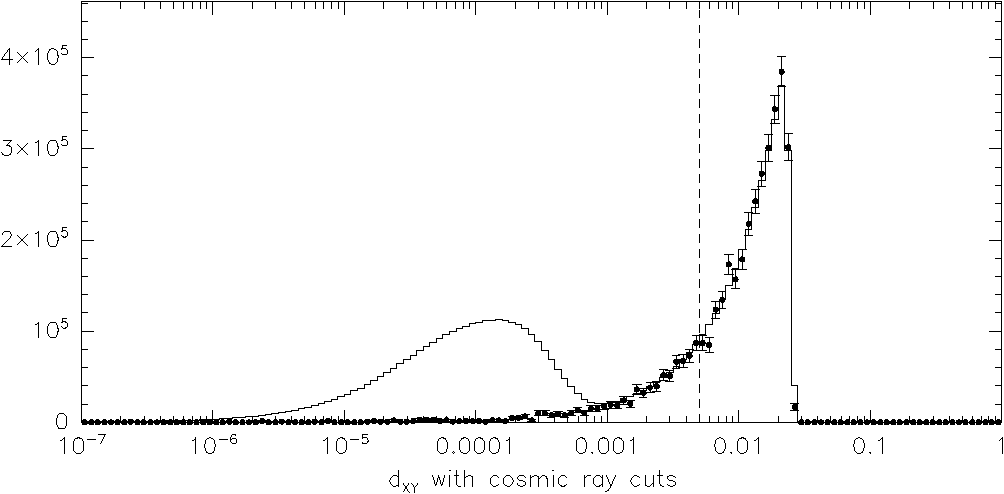
\includegraphics[width=\linewidth]{plots/dxydzcontaminationa}
  \end{center}
  \caption{\label{dxydzcontaminationa} Distance from the beam-line
  ($|d_{XY}|$ in $\log x$-scale, where 1 = one meter) with all other
  cosmic ray cuts applied.  Data from beam-beam collisions are the
  solid histogram with a peak at 0.0001 (0.1~mm) and 0.01 (10~cm) from
  cosmic rays.  Data from the no-beam sample are the points with error
  bars, normalized to equal numbers of cosmic rays.  The dashed
  vertical line is the cut boundary at 5~mm.  Triggers fail to accept
  cosmic rays beyond 25~cm.}
\end{figure}

Beam-gas and beam-wall events are hard to distinguish from one
another, but they are both small backgrounds which depend on the
electron and positron beam currents.  This dependence is not
identical, since beam-gas rates are proportional to the gas pressure
inside the beam-pipe while beam-wall is not.  However, the
contamination from beam-gas and beam-wall combined is typically 0.2\%
of the continuum.  Furthermore, our beam-gas and beam-wall cuts have a
small background from beam-beam data, meaning that our 0.2\% estimate
is too large.  Instead of subtracting this number, we inflate our
uncertainty by this amount.

To identify beam-gas and beam-wall events (which we will call
beam-nucleus), we require
\begin{itemize}

  \item \dxy\ $<$ 5~mm, \dz\ $>$ 7.5~cm,

  \item $|\vec{p}_1 \cdot \vec{p}_2| / |\vec{p}_1| |\vec{p}_2|$ $<$
    0.9 to further reject cosmic rays,

  \item at least two tracks, and \visen\ $>$ 4\% of \ecm.

\end{itemize}
To distinguish between electron-induced beam-nucleus and
positron-induced beam-nucleus events, we also cut on the net
$z$-momentum of all tracks ($p_z^\subs{tr}$).  For a positron-induced
event, we require $p_z^\subs{tr}$ $>$ 10\% of \ebeam\ because incident
positron momentum is in the positive $z$ direction (see Figure~\ref{coordinatesystem}).  Electron-induced events must have
$p_z^\subs{tr}$ $<$ $-$10\% of \ebeam.

To relate the number of identified beam-nucleus events to the number
that contaminate our hadronic event count, we employ data samples
acquired with only one beam in CESR (also listed in
Table~\ref{tab:controls}).  To use these samples, we must first
subtract the cosmic rays using the technique described above.
Figure~\ref{beamgaspz} demonstrates the separation of electron- and
positron-induced beam-nucleus by their net $z$-momenta.  This Figure
also indicates that a small fraction, perhaps 10\%, of our
beam-nucleus candidates are contaminated by beam-beam events, probably
two-photon fusion with a misreconstructed \dz.  The potential for
contamination is also evident in Figure~\ref{dxydzcontaminationb}.
Therefore, a beam-nucleus correction in analogy with the cosmic ray
correction would be an over-subtraction of about 10\%.  The
beam-nucleus estimates are typically only 0.1\% of the continuum
(Figure~\ref{backgroundsvsrun}), so we subtract 50\% \PM\ 50\% of the
electron- and positron-induced beam-nucleus estimates.  The effective
cross-section of beam-nucleus estimates are plotted near the bottom of
Figure~\ref{awesome}.  The cosmic ray and beam-nucleus estimates for
every run we used to determine \gee\ are plotted in
Figure~\ref{backgroundsvsrun}.

\begin{figure}[p]
  \begin{center}
    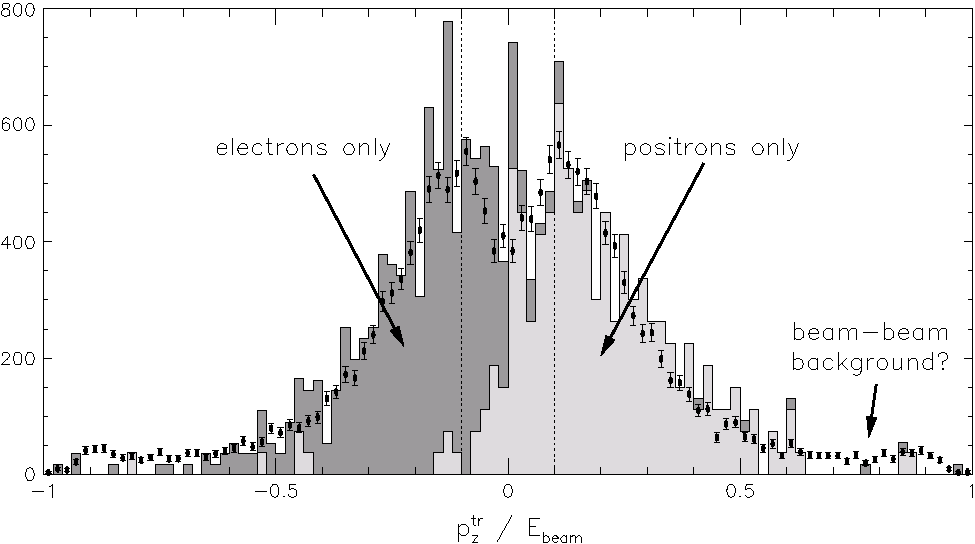
\includegraphics[width=\linewidth]{plots/beamgaspz}
  \end{center}
  \caption{\label{beamgaspz} Net $z$-momentum of all tracks
  ($p_z^\subs{tr}$) with all other beam-nucleus cuts applied.  Data
  with only positrons in CESR are lightly-shaded, electrons-only are
  darkly-shaded and stacked on the positrons-only histogram, and data
  from collisions are represented by points with error bars.  The
  boosts imparted by the incident beams are evident, and dotted
  vertical lines at $\pm$10\% of \ebeam\ indicate cuts for electron-
  and positron-induced beam-nucleus events.  The beam-beam data do not
  exactly reproduce the combined distribution, though the
  electrons-only and positrons-only histograms have been normalized to
  the same totals above and below $\pm$10\% of \ebeam.}
\end{figure}

\begin{figure}[p]
  \begin{center}
    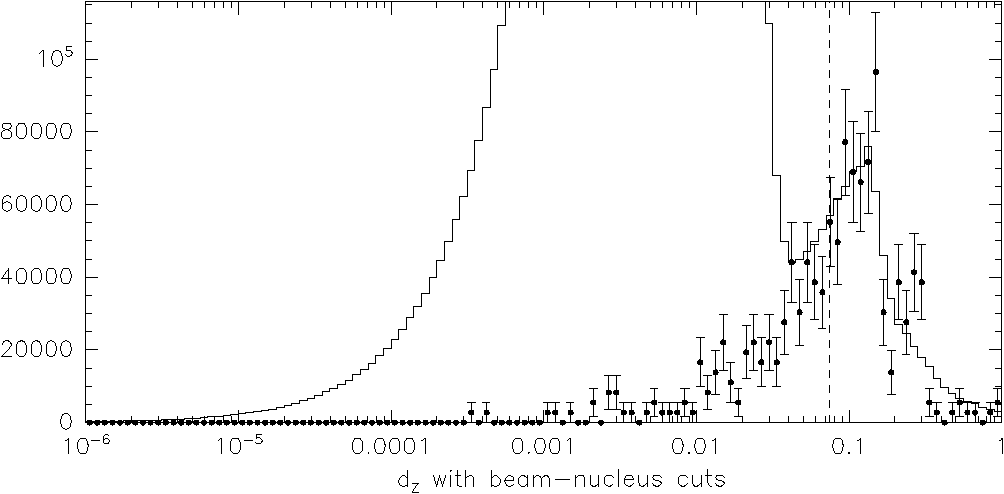
\includegraphics[width=\linewidth]{plots/dxydzcontaminationb}
  \end{center}
  \caption{\label{dxydzcontaminationb} Distance of the $z$ event
  vertex from the center of the beam-beam distribution ($|d_Z|$ in
  $\log x$-scale, where 1 = one meter).  Data from beam-beam
  collisions are the solid histogram with a peak above the plot window
  at 0.01 (1~cm) and a peak at 0.1 (10~cm) from beam-nucleus
  collisions.  Data from the single-beam samples are the points with
  erorr bars, normalized to equal numbers of beam-nucleus events.
  Cosmic rays have been subtracted from both samples.  The dashed
  vertical line is the cut boundary at 7.5~cm.}
\end{figure}

\begin{figure}[p]
  \begin{center}
    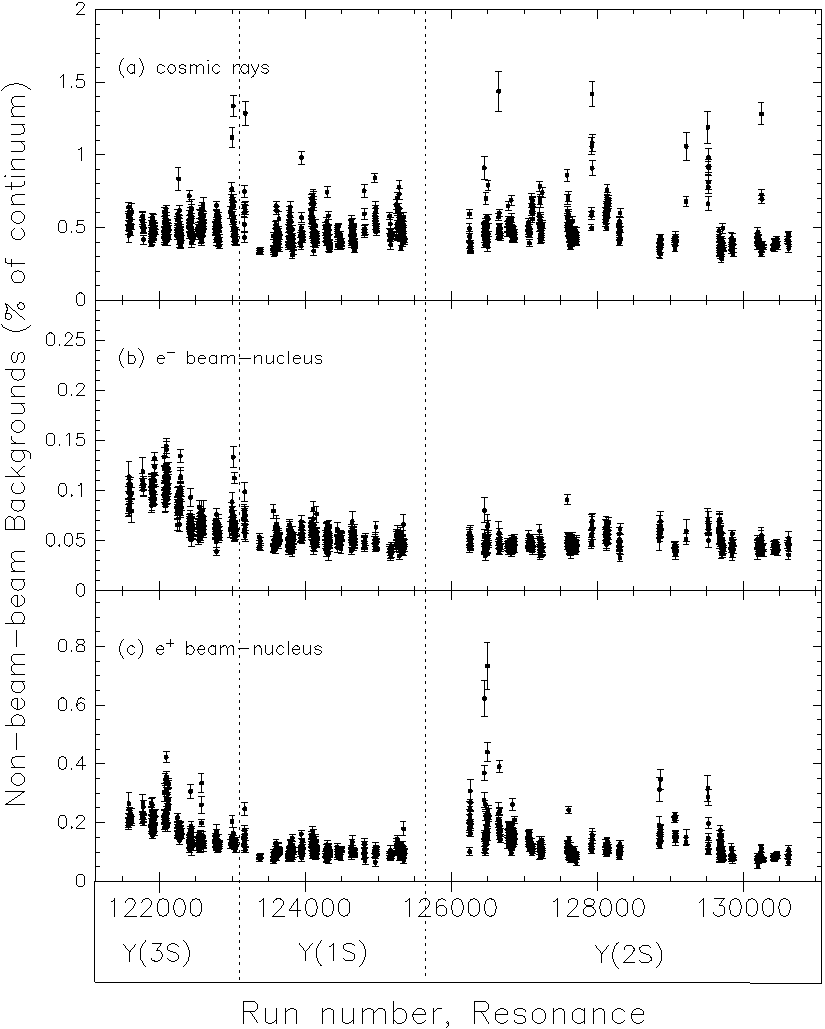
\includegraphics[width=0.9\linewidth]{plots/backgroundsvsrun}
  \end{center}
  \caption{\label{backgroundsvsrun} Total counts of non-beam-beam
  backgrounds as a fraction of the continuum level and a function of
  run number.  Dashed vertical lines separate \usss, \us, and \uss\
  data-taking periods.  Note that all three plots have different
  vertical scales: cosmic rays are the most abundant, and the
  proportion of positron-induced beam-nucleus events are typically
  twice that of electron-induced events.}
\end{figure}

\chapter{Hadronic Efficiency}
\label{chp:efficiency}

\section{Motivation for the Data-Based Approach}

Inefficiency is in some sense the opposite of the problem of
backgrounds: after removing the events which should not be in our
hadronic \ups\ sample, we need to add in the events that are missing.
In this Chapter, we will determine the probability that a hadronic
\ups\ decay is included in our count, for each of the three
resonances.  These efficiencies are high, about 97\% for each
resonance.

Often, efficiencies are determined from Monte Carlo simulations.  One
simulates all known decay modes, and constructs an aggregate efficiency
\begin{equation}
  \epsilon = \sum_i \, \epsilon_i \, {\mathcal B}_i \mbox{,}
  \label{eqn:agregate}
\end{equation}
where $\epsilon_i$ is the efficiency of each mode.  We don't directly
use this method for two reasons.
\begin{enumerate}

  \item Hadronic decays are the result of the hadronization of bare
    quarks and gluons.  This is a non-perturbative process which is
    only empirically approximated by LUND/JetSet in the Monte Carlo.
    If we assume a non-perturbative QCD model to determine a
    non-perturbative QCD parameter, we would introduce a circular
    dependence that would have to be quantified.

  \item Our definition of hadronic \ups\ decays includes potentially
    unknown modes whose efficiencies may be very different from the
    hadronic modes we simulate.  For instance, it is possible that
    \ups\ decays into invisible $\mbox{\sc wimp}$s with zero
    efficiency or that unknown QCD resonances may enhance decays to
    $K_L$ or neutrons, which fail our \visen\ cut with greater
    probability.

\end{enumerate}

Instead, we take advantage of a 1.3 fb\inv\ sample of \uss\ decays to
study \twotoone\ transitions.  The \us\ mesons in these decays are
produced nearly at rest, and decay as they would from direct $e^+e^-
\to \Upsilon(1S)$.  However, the $2S \to 1S$ cascade events
additionally include two charged pions which may satisfy a trigger
algorithm and cause the event to be recorded, regardless of how the
\us\ decays.  As an extreme example, we can use this technique to
collect events featuring invisible $\Upsilon(1S) \to \nu\bar{\nu}$
decays, which would be impossible with a direct \us\ sample.

We exploit this broad access to \us\ decays to measure the \us\
efficiency.  From \twotoone\ cascades, we select a subset in which the
\pipi\ by itself guarantees that the trigger will accept the event, so
that we know that the trigger did not rely on decay products of the
\us.  Assuming that there is no correlation between the kinematics of
the \pipi\ and the branching fractions of the \us, this subset of
\pipi\ is accompanied by a generic set of \us\ decays: \us\ decay
modes are represented in the data sample with the same proportions as
in nature.  We may then apply our cuts to the \us\ decay products in
our sample to determine the fraction which succeed.  This is the
efficiency.

\section{Hadronic Efficiency of the \boldmath \us}
\label{sec:usefficiency}

We have two goals for our event selection in this study, to identify
\twotoone\ candidates and to choose \pipi\ candidates which are
sufficient to satisfy the trigger.  The \pipi\ in \twotoone\ are
kinematically constrained by the mass difference between the \uss\ and
the \us, so the mass of the system recoiling against the two pions,
\begin{equation}
  {m_\subs{$\pi\pi$-rec}}^2 = \left(M_{\Upsilon(2S)} - \sqrt{|\vec{p}_1|^2 + {m_\pi}^2}
  - \sqrt{|\vec{p}_2|^2 + {m_\pi}^2}\right)^2 - |\vec{p}_1 + \vec{p}_2|^2 \mbox{,}
  \label{eqn:mrec}
\end{equation}
peaks at the \us\ mass.  This allows for excellent background
rejection, because the peak from \twotoone\ has a 3~MeV resolution
while the background spectrum is much broader (see Figure~\ref{cascadescartoon}).  We require \pipi\ candidates to have a recoil
mass ($m_\subs{$\pi\pi$-rec}$) between 9.441 and 9.480~GeV.  We
further suppress background by requiring the track helices that we
identify as \pipi\ to intersect in the $x$-$y$ plane within 5~mm of
the nominal beam-beam collision point.  The track helices at this $x$-$y$
point must also be less than 2.5~cm from each other in $z$, and their
average $z$ must be within 5~cm of the beam-beam collision point.  The
momenta used in Equation~\ref{eqn:mrec} are evaluated at the
intersection point.

\begin{figure}[t]
  \begin{center}
    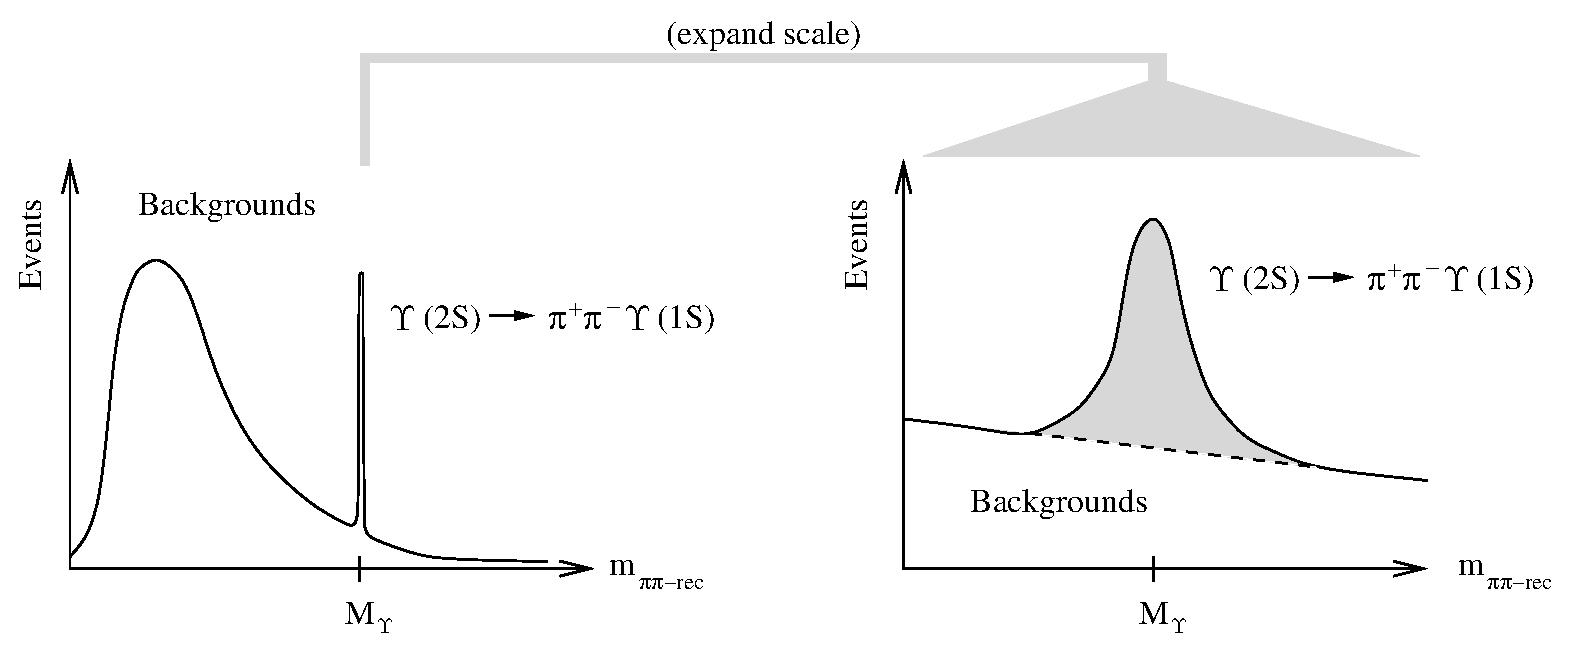
\includegraphics[width=\linewidth]{plots/cascadescartoon}
  \end{center}
  \caption{\label{cascadescartoon} Distinguishing the recoil mass of
  \pipi\ in kinematically-constrained \twotoone\ events from other,
  accidental track-track combinations (backgrounds).  The background
  distribution is not simple, but it has no structure in the narrow
  region of our interest.}
\end{figure}

To satisfy the trigger, we select \pipi\ track candidates with more
than 150~MeV of momentum perpendicular to the $z$ axis ($p_\perp$), so
that their trajectories reach beyond the sixteenth layer in the drift
chamber and satisfy the geometric requirements for \axial\ tracks.  A
study of CLEO's trigger response to hadronic tracks revealed that the
probability for a track with $p_\perp$ $=$ 150~MeV to be detected as an
\axial\ track is 99.96\%, and this probability grows with $p_\perp$.
We can therefore be at least 99.92\% certain that events accepted by
the \twotrack\ trigger (which requires two \axial\ tracks) with this
cut on the \pipi\ did not rely on \us\ decay products to be accepted.

To simplify the process of excluding the \pipi\ candidates when we
apply our hadronic cuts, we additionally require each pion track to
have more than 60~MeV of $z$-momentum magnitude.  As discussed in
Section \ref{pag:spiraling} on page \pageref{pag:spiraling}, such
trajectories exit the detector before completing one half-orbit in the
magnetic field.  This protects our sample from events with pions which
spiral in the tracking volume, potentially generating many tracks,
only one of which is identified as a pion from \twotoone.  With this
cut, we can assume that each pion is responsible for only one track
and the calorimeter showers associated with that track.

There is occasionally more than one pair of tracks which satisfy these
\pipi\ criteria in a single event.  In this case, we choose a \pipi\
candidate randomly.  If we were to choose the \pipi\ candidate that
best reconstructs the \us\ mass, would could bias the non-cascade
background to peak under the \twotoone\ signal, complicating the
background subtraction.  Since the \pipi\ candidate is chosen
randomly, the background distribution has no structure on the scale of
tens of MeV, and we can approximate it with a Taylor expansion, as
shown in Figure~\ref{cascadescartoon}.

If we select \twotoone\ candidates in this manner, from events
accepted by the \twotrack\ trigger, and apply our hadronic cuts to the
\us\ events in the peak, we find a hadronic \us\ efficiency that is
consistent with 100\% with a 3\% uncertainty, and this is not
satisfactory for our analysis.  Hadronic efficiency is a factor in
\geehadtot, so the fractional uncertainty in hadronic efficiency adds
to the \geehadtot\ fractional uncertainty in quadrature.

The main culprit is the prescaled \twotrack\ trigger, which randomly
rejects 94.7\% of the events which satisfy its two \axial\ track
criteria.  We can circumvent this loss of data and improve the
precision of our result by splitting the \us\ hadronic efficiency into
two factors.  Define an \us\ decay as ``visible'' if the trigger
records one \axial\ track from the \us\ decay products and one \cblo\
cluster from either the \us\ decay or the \pipi.  Define \evis\ to be
the probability that an \us\ decay is visible, and \ecuts\ to be the
probability that a visible \us\ decay is selected by our triggers and
cuts.  The hadronic \us\ efficiency is the product of \evis\ and
\ecuts.  We will determine \evis, a number which is very close to
100\%, using the \twotrack\ trigger, and \ecuts\ using the \hadron\
trigger, which selects visible \us\ decays accompanied by \pipi.
Since $(1-\epsilon_\subs{vis})$ is such a small inefficiency, a large
fractional uncertainty in $(1-\epsilon_\subs{vis})$ propagates to a
small fractional uncertainty in \evis.

Our definition of ``visible'' is tailor-made for the \hadron\ trigger
in \twotoone\ events.  The \hadron\ trigger requires three \axial\
tracks and one \cblo\ cluster.  We have selected \pipi\ kinematics
such that each pion must generate one \axial\ track, so the \us\ decay
is responsible for the third track and possibly the \cblo.  Whatever
the probability is that the \cblo\ comes from the \pipi, rather than
the \us, it is the same while measuring \evis\ as it is while
measuring \ecuts.  This gives us the freedom to determine the cut
efficiency with a large set of events from the \hadron\ trigger,
knowing that we can correct for the bias it introduces with \evis.

In our article in Physical Review Letters, we discussed this technique
more succinctly using two factors, $\epsilon_\subs{htrig}$ and \ecuts.
In that article, $\epsilon_\subs{htrig}$~=~\evis\ here, and \ecuts\
has the same meaning in both.

\subsection{Determination of \boldmath \evis}

To determine \evis, we apply the above procedure, replacing our full
set of cuts for the ``visible'' condition we have just defined.  The
recoil mass distribution of \pipi\ candidates accepted by the
\twotrack\ trigger is shown in Figure~\ref{pipitwotrack}(a).  The real
\twotoone\ events peak near the \us\ mass of 9.46~GeV, and backgrounds
are distributed linearly underneath.  To measure the fraction of \us\
decays that are ``invisible,'' we select from this sample events that
fail the \hadron\ trigger.  These are plotted in Figure~\ref{pipitwotrack}(b), revealing no significant peak.  This indicates
that nearly all of the \us\ decays are visible.

\begin{figure}[p]
  \begin{center}
    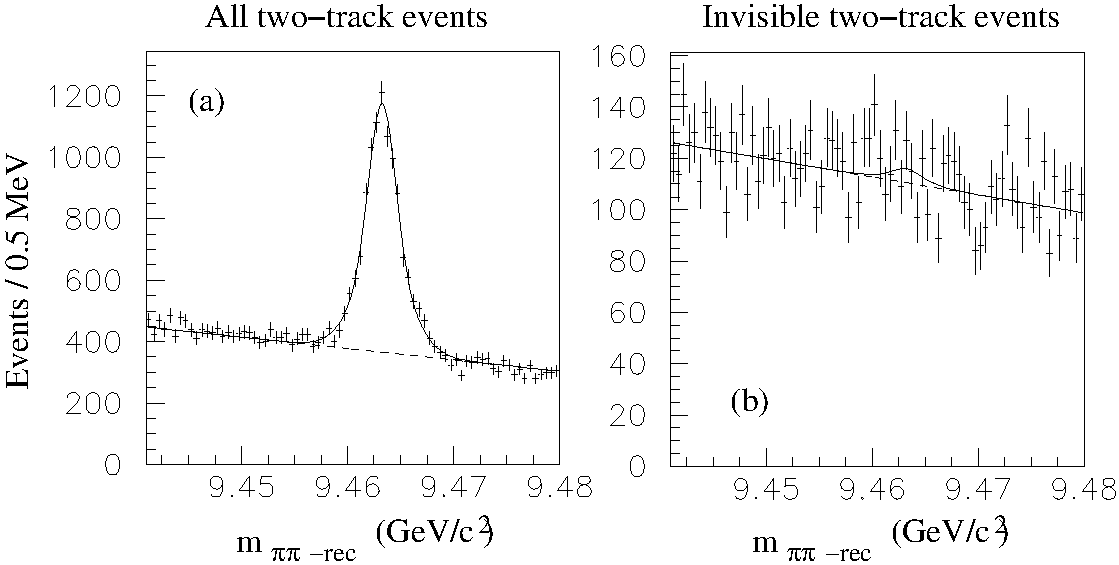
\includegraphics[width=\linewidth]{plots/pipitwotrack}
  \end{center}
  \caption{\label{pipitwotrack} Recoil mass of \pipi\ candidates for
  (a) all events accepted by the \twotrack\ trigger, and (b) only
  those in which the rest of the event is ``invisible.''  True
  \twotoone\ events are contained in the peak near 9.46~GeV, which is
  highly suppressed in (b), indicating that very few \us\ decays are
  invisible.  The solid curve is a fit to the data, and the dashed
  curve is the linear background contribution.}
\end{figure}

To quantify this statement, we fit the data in Figures
\ref{pipitwotrack}(a) and \ref{pipitwotrack}(b) to the same function and
extract the ratio of \twotoone\ yields.  We fit the full \twotrack\
dataset (Figure~\ref{pipitwotrack}(a)) to a double Gaussian with a 1:4
ratio of areas and a linear background.  When we fit the
invisible-\us\ data (Figure~\ref{pipitwotrack}(b)), we fix the mean and
widths, imposing the assumption that momentum resolution of the \pipi\
is independent of the visibility of the \us.  This very reasonable
assumption purchases much of the statistical precision in the
measurement.  The ratio of fit yields is (0.67 \PM\ 0.62)\%.  The
0.2\% branching fraction of \us\ to $\nu\bar{\nu}$ we discussed
earlier is included in this inefficiency, but is smaller than its
statistical uncertainty.

This ratio of fit yields represents the fraction of \us\ decays that
are invisible, including leptonic \us\ decays.  Leptonic decays,
particularly \ee\ and \mumu, are more likely to be invisible than
hadronic decays, since their final state consists of only two
particles which are geometrically back-to-back: if one lepton
disappears down the beam-pipe, the other probably will do so on
the other side.  We determine the probability for leptons to be
invisible from leptonic Monte Carlo simulations (which include the
$(1+\cos\theta)$ angular distribution for leptonic decays through a
virtual photon), and this probability is (10.91 \PM\ 0.01)\%.  We use
Equation \ref{eqn:agregate} to determine the hadronic visibility
efficiency, \evis, from the total visibility efficiency
($\epsilon_\subs{vis}^\subs{tot} = 1 - 0.0067$) and the leptonic
visibility efficiency ($\epsilon_\subs{vis}^\subs{lep} = 1 - 0.1091$).
\begin{equation}
  \epsilon_\subs{vis} = \frac{\epsilon_\subs{vis}^\subs{tot} - \epsilon_\subs{vis}^\subs{lep} \times (3{\mathcal B}_{\mu\mu})}{(1 - 3{\mathcal B}_{\mu\mu})}
%  = \frac{(1 - 0.0067) - (1 - 0.0011)(3{\mathcal B}_{\mu\mu})}{(1 - 3{\mathcal B}_{\mu\mu})}
  = (100.02 \pm 0.62)\% \mbox{.}
  \label{eqn:leptoniccorrection}
\end{equation}
Slightly more than half of this probability distribution is above
100\%, which is impossible for a real efficiency, so we truncate the
part above 100\% and normalize the remaining distribution to obtain an
asymmetric uncertainty: \evis\ = (99.59 $^{+0.29}_{-0.45}$)\%.

\subsection{Determination of \boldmath \ecuts}

We select \pipi\ candidates in the same way to determine \ecuts,
except that we choose events accepted by the \hadron\ trigger rather
than the \twotrack\ trigger.  Figure~\ref{pipihadron}(a) presents the
recoil mass of these \pipi\ candidates, recoiling against visible \us\
decays.  We apply our hadronic cuts (but not the trigger requirements)
to this sample, excluding tracks and showers associated with the
\pipi, and plot the recoil mass for these in Figure~\ref{pipihadron}(b).  These ``cut-failure'' events have a prominent
peak at the \us\ mass due to all the visible \us\ events which failed
our cuts.  (Most of them are leptonic decays.)

\begin{figure}[p]
  \begin{center}
    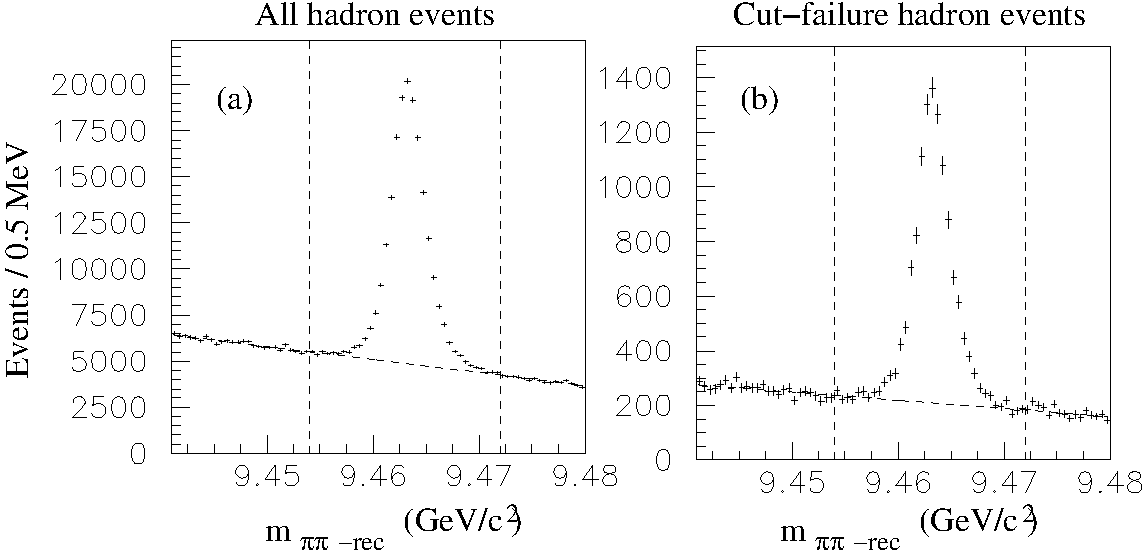
\includegraphics[width=\linewidth]{plots/pipihadron}
  \end{center}
  \caption{\label{pipihadron} Recoil mass of \pipi\ candidates for (a)
  all events accepted by the \hadron\ trigger, and (b) only those in
  which the rest of the event fails our cuts (``cut-failure'' events).
  The dotted vertical lines identify the signal region, and the dashed
  curve is a fit to the background, used to subtract background events
  from the signal region.}
\end{figure}

To obtain the ratio of cut-failure \us\ events to all visible \us\
events, we avoid the fit procedure because of the potential for
systematic uncertainties in the fit parameterization.  In the \evis\
study, the statistical uncertainty in the number of invisible events
was almost as large as the number of invisible events itself, and this
overwhelmed any bias introduced by the fit function shape.  Here, the
number of cut-failures is significantly greater than zero and ought to
be measured more precisely.  Instead of fitting, we count events with
a recoil mass between 9.454 and 9.472~GeV and subtract the 
backgrounds, which have been determined by a linear fit to the sidebands
(between 9.441 and 9.480 GeV, excluding the signal region).  To
estimate the systematic uncertainty in yield due to assuming a linear
background, we repeat the procedure with the largest quadratic term
allowed by the data.

The ratio of cut-failure \us\ events to all visible \us\ events is
(92.58 \PM\ 0.13 \PM\ 0.02)\%, where the first uncertainty is
statistical and the second is due to the parameterization of the
background distribution.  The leptonic modes account for most of this
7\% inefficiency: correcting for leptonic modes as above
(Equation~\ref{eqn:leptoniccorrection}) yields \ecuts\ = (98.32 \PM\
0.21)\%.

The apparent \us\ efficiency, measured in \twotoone\ cascades, may
differ from the efficiency of direct $e^+e^- \to \Upsilon(1S)$ events
because of the slight relativistic boost ($\gamma = 1.005$) or the
potential for \pipi\ showers to overlap \us\ showers in cascade
decays.  To address these possibilities, we generate hadronic Monte
Carlo for the direct and the cascade cases, applying the same
procedure to determine the hadronic efficiency from the cascade
simulation.  We observe no significant difference: the ratio of direct
efficiency to cascade efficiency is 1.0014 \PM\ 0.0022.  We apply this
as a correction primarily to propagate the uncertainty in this study.

Incidentally, the cascade Monte Carlo prediction of \ecuts, (98.54
\PM\ 0.22)\%, agrees with our data-based measurement of (98.32 \PM\
0.21)\%.  We would have been correct, if not justified, if we had
derived our cut efficiency directly from the Monte Carlo.  We also
extract \pmax, \visen, \dxy, and \dz\ from our cascade data and
cascade Monte Carlo, and find that they agree fairly well (Figure~\ref{cascadeagreement}).

\begin{figure}[p]
  \begin{center}
    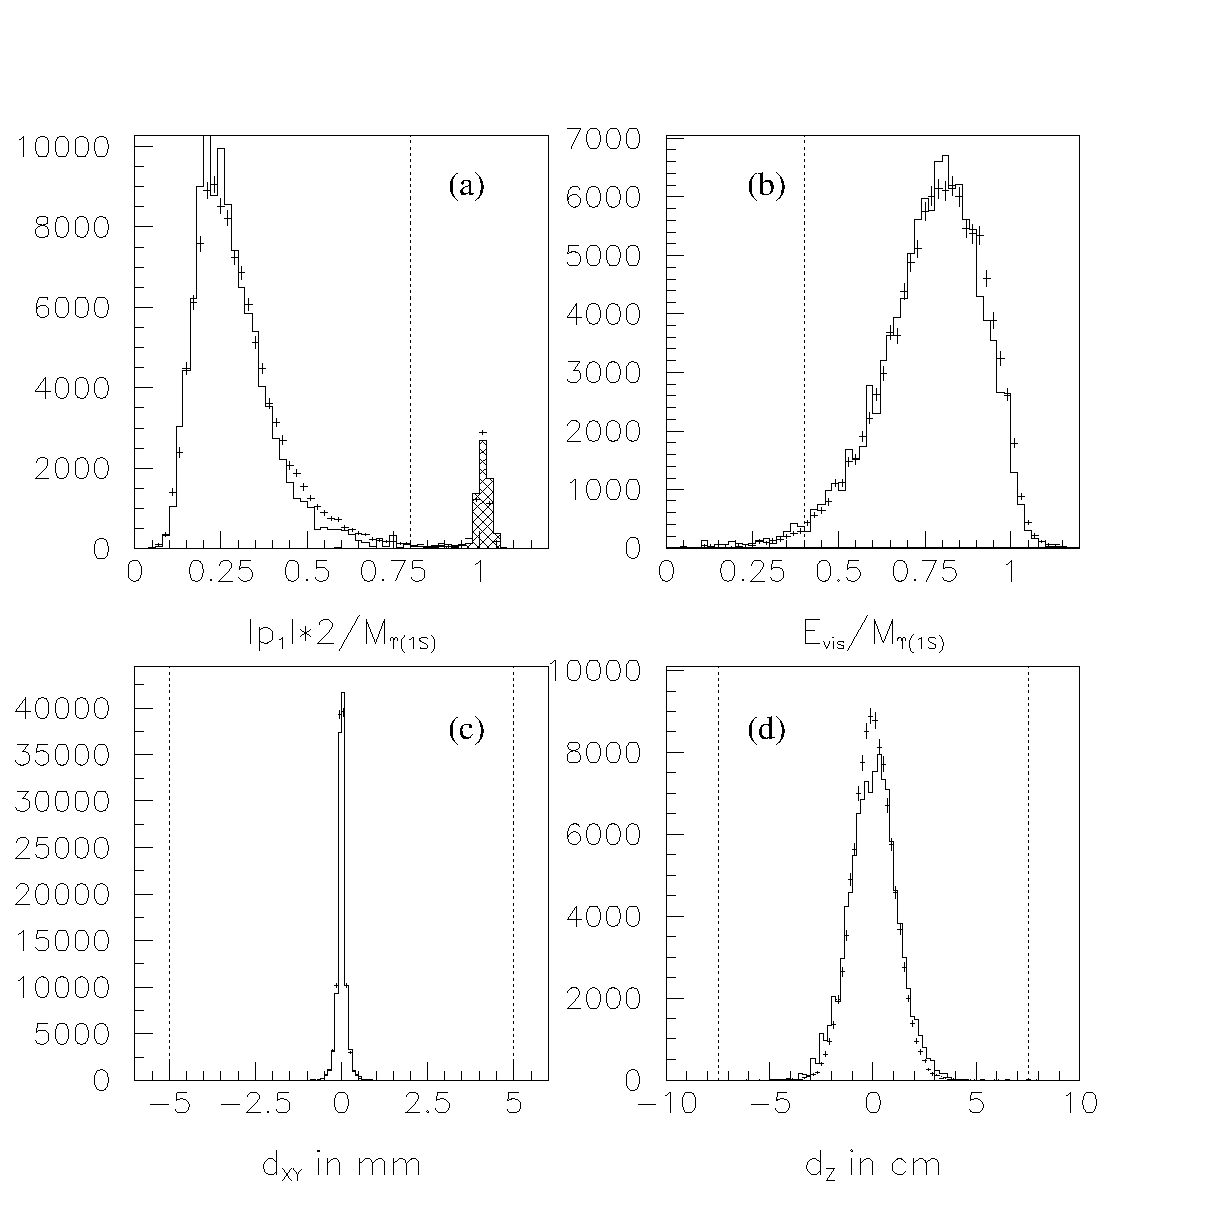
\includegraphics[width=\linewidth]{plots/cascadeagreement}
  \end{center}
  \caption{\label{cascadeagreement} Our four cut variables, as seen in
  background-subtracted \twotoone\ events.  Points with errorbars are
  data, the solid histograms are \twotoone\ Monte Carlo simulations
  with the same procedure applied, and the dotted vertical lines are
  the cut thresholds.  (a) Largest track momentum (\pmax), divided by
  $M_\Upsilon/2$, the equivalent of \ebeam\ if this were a direct
  decay.  The peak at 1 is due to \ee\ and \mumu\ decays,
  cross-hatched in the Monte Carlo.  (b) Visible energy (\visen),
  divided by $M_\Upsilon$, the equivalent of \ecm.  (c) The distance
  of the closest track to the beam-line (\dxy).  (d) The $z$-vertex of
  the event (\dz).}
\end{figure}

One correction is still missing from the \ecuts\ we have derived:
\ecuts\ must include the trigger efficiency, but we excluded trigger
requirements from our measurement.  While we can remove the \pipi\
tracks and showers from our fully reconstructed data, it would be
impractical to apply an analogous procedure on our trigger data for
technical reasons.  We therefore use Monte Carlo to determine the
efficiency of the trigger once our cuts have been applied, a value of
99.87\%.  Figure~\ref{triggeragreement} overlays data and Monte Carlo
\axial, \stereo, \cblo, and \cbmd\ distributions in direct \us\
decays, showing fairly good agreement.  The predicted inefficiency of
0.13\% can therefore be trusted within 100\% of itself, so we
conservatively assign this as the systematic uncertainty.

\begin{figure}[p]
  \begin{center}
    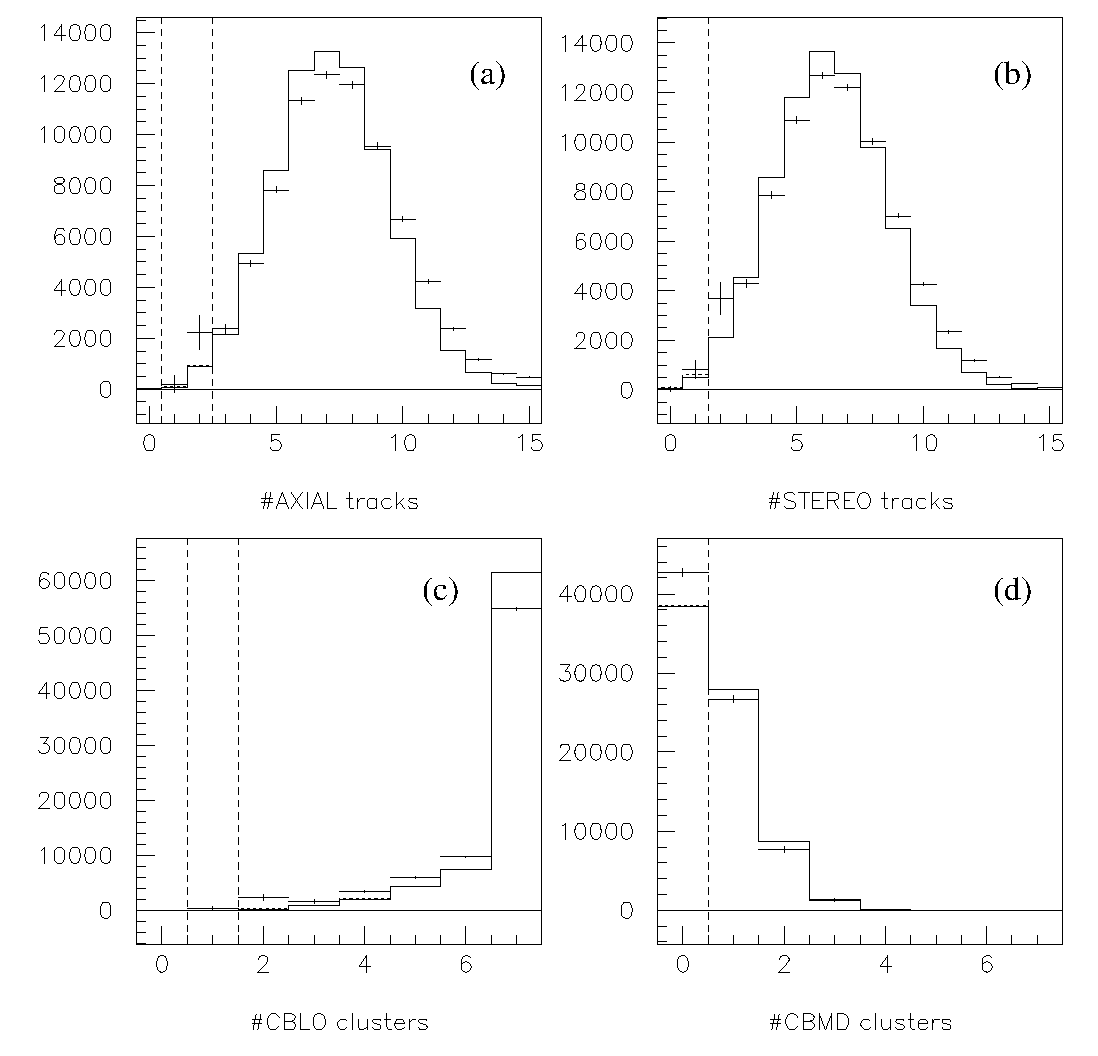
\includegraphics[width=\linewidth]{plots/triggeragreement}
  \end{center}
  \caption{\label{triggeragreement} The four cut variables used in
  \hadron, \radtau, and \eltrack\ trigger decisions (defined on page
  \pageref{pag:triggerdefs}).  Points with errobars are
  continuum-subtracted data, histograms are Monte Carlo simulations,
  and the dashed vertical lines are cut thresholds.  Trigger
  selections have been applied to data and Monte Carlo, though Monte
  Carlo without trigger selections are overlaid as dotted histograms
  (barely visible).}
\end{figure}

After all of these corrections, the efficiency of visible hadronic
\us\ decays is \ecuts\ = (98.33 \PM\ 0.33)\%.  The efficiency of all
hadronic \us\ decays is \evis~$\times$~\ecuts\ = (97.93
$^{+0.44}_{-0.56}$)\%.

\section{Hadronic Efficiency of the \boldmath \uss\ and \usss}
\label{sec:ussusssefficiency}

The $\Upsilon(3S) \to \pi^+\pi^- \Upsilon(2S)$ and $\Upsilon(4S) \to
\pi^+\pi^- \Upsilon(3S)$ rates are too low to accumulate large samples
to study \uss\ and \usss\ efficiencies in the same way that we did
\us.  Instead, we derive correction factors from the Monte Carlo that
allow the \us\ efficiency to be applied to the \uss\ and \usss.

The decays of the \uss\ and \usss\ differ from those of the \us\ in
two ways.  The \uss\ and \usss\ decay products are slightly more
energetic, as they originate in a state of higher \ecm, and the \uss\
and \usss\ can decay via transitions to lower $b\bar{b}$ resonances.
The first correction is very small because our \pmax\ and \visen\ cut
thesholds are constant fractions of \ecm, and the difference in \ecm\
from \us\ to \usss\ is only 10\%.  In the Monte Carlo simulation, the
\uss\ and \usss\ efficiency for \ggg, \gggamma, and \qqbar\ is only
0.2\% lower than the \us\ efficiency.

Most \uss\ and \usss\ transition decays have the same efficiency as
\ggg, \gggamma, and \qqbar, so they have no impact on total hadronic
efficiency.  The exceptions are transitions that result in a lower
\ups\ resonance decaying into \ee\ or \mumu.  According to the Monte
Carlo simulation, these ``cascade-to-leptons'' decays have (0.69 \PM\
0.22)\% efficiency for \uss\ and (0.38 \PM\ 0.19)\% efficiency for the
\usss--- almost zero.  Therefore the efficiency correction will be
approximately $(1 - {\mathcal B}_\subs{cas})$, where \bcas\ is the
branching fraction for these modes.

We determine this branching fraction from the data by counting
cascade-to-leptons events relative to $\Upsilon \to \mu\mu$ in the
full \uss\ and \usss\ datasets.  We select all events that have two
high-momentum tracks ($|\vec{p}| >$ 70\% \ebeam) without associated
high-energy showers ($E_\subs{max} <$ 70\% \ebeam), that is,
consistent with two high-energy muons accompanied by anything.  We
plot the invariant mass of these two muons in Figure~\ref{invariantmumass}, after subtracting continuum processes using the
off-resonance data.  Muon pairs from direct \ups\ decays are easily
distinguished from cascade-to-leptons events.  The Monte Carlo
reproduces the invariant mass spectrum with only tiny errors in the
calibration of the magnetic field (a horizontal shift in the plot).

\begin{figure}[p]
  \begin{center}
    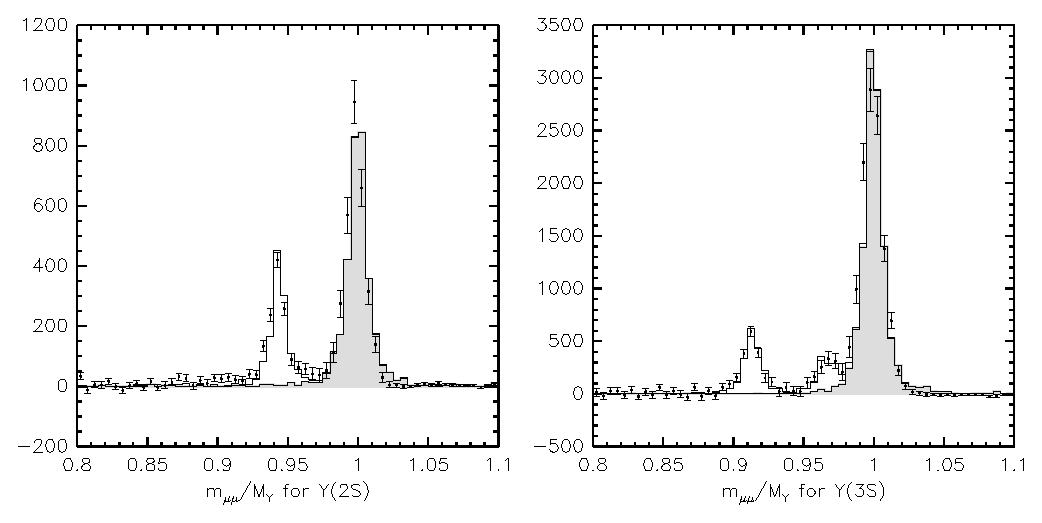
\includegraphics[width=\linewidth]{plots/invariantmumass}
  \end{center}
  \caption{\label{invariantmumass} Invariant mass spectra of \mumu\ in
  events with two energetic muons.  Points with errorbars are
  continuum-subtracted data, and histograms are Monte Carlo
  simulations, with prompt $\Upsilon \to \mu^+\mu^-$ shaded.  The
  horizontal shift in energy scale is consistent with the uncertainty
  in our magnetic field estimate.}
\end{figure}

We measure \bcas\ relative to \bmm\ by fitting Monte Carlo
cascade-to-muon pairs and Monte Carlo direct muon pairs to the data in
Figure~\ref{invariantmumass}.  This fit has two free parameters, the
magnitude of \bcas\ and the magnitude of \bmm.  We assign conservative
10\% uncertainties to this procedure, which overwhelm \bmm\
uncertainties and yield only 0.1\% uncertainties in the final
efficiency determination.  The resulting \bcas\ for \uss\ is (1.58
\PM\ 0.16)\% and for \usss\ is (1.34 \PM\ 0.13)\%, accounting for the
factor of two from cascade-to-electron pairs.

Applying these corrections to the \uss\ and \usss\ efficiencies, we
obtain (96.18 $^{+0.44}_{-0.56}$ \PM\ 0.15)\% and (96.41
$^{+0.44}_{-0.56}$ \PM\ 0.13)\% for the \uss\ and \usss, respectively.
The first uncertainty is derived from the \twotoone\ study and is
common to all three resonances.  The second uncertainty arises from
our \bcas\ measurements and is independent for the \uss\ and \usss.
The first uncertainty therefore cancels in ratios of \gee, while the
second does not.

\chapter{Integrated Luminosity}
\label{chp:luminosity}

Now that we can reliably count the number of hadronic \ups\ decays at
every \ecm\ we sampled, we need to determine the hadronic
cross-section this implies by measuring the integrated luminosity of
the same data.  We get the integrated luminosity from a count of
Bhabha events, since these are plentiful and their rate can be
accurately calculated from perturbative QED.  Integrated luminosity is
the ratio of Bhabha events counted to the efficiency-weighted Bhabha
cross-section, and the hadronic \ups\ cross-section is the ratio of
hadronic \ups\ events to the integrated luminosity.

Any theoretically calculable process can be used to determine the
integrated luminosity; Bhabhas were chosen primarily for their
abundance, since this minimizes statistical uncertainty.  A Bhabha
count is complicated by the fact that $\Upsilon \to e^+e^-$ is
indistinguishable from Bhabhas on an event-by-event basis, and this
background is a sharp function of \ecm.  Alternatively, one could
determine the integrated luminosity from $e^+e^- \to \gamma\gamma$
because $\Upsilon \not\to \gamma\gamma$ (electromagnetic decays do not
violate parity).  Unfortunately, this comes at the cost of a factor of
eight (\borky) in statistics.  The $\Upsilon \to e^+e^-$ contribution
can easily be controlled, and the additional statistical power is
valuable when determining ratios of \gee$(nS)$/\gee$(mS)$, so we
determine integrated luminosities from Bhabhas and use \gamgam\ events
as a cross-check.

\section{Bhabha Count and \boldmath \gamgam\ count}

To select Bhabha events, we require
\begin{itemize}

  \item two or more tracks with momenta between 50\% and 110\% of
    \ebeam, and an energy sum (including showers from bremsstrahlung
    radiation as the electrons propagate through the detector) of more
    than 90\% \ecm.

  \item The larger (smaller) track $|\cos\theta|$ must be less than
    0.766 (0.707), and

  \item each track must be associated with a calorimeter shower, with the
    larger (smaller) shower energy divided by track momentum
    ($E_\subs{shower}/|\vec{p}_\subs{track}|$) being greater than 80\%
    (50\%).

\end{itemize}
With these cuts, backgrounds other than $\Upsilon \to e^+e^-$ are
negligible.  Different thresholds are set for the larger and smaller
angles and calorimeter energies to reduce sensitivity to the threshold
values, and possible efficiency variation with time.  See Figure~\ref{asymmetriccartoon} for an illustration of this kind of cut.

\begin{figure}[p]
  \begin{center}
    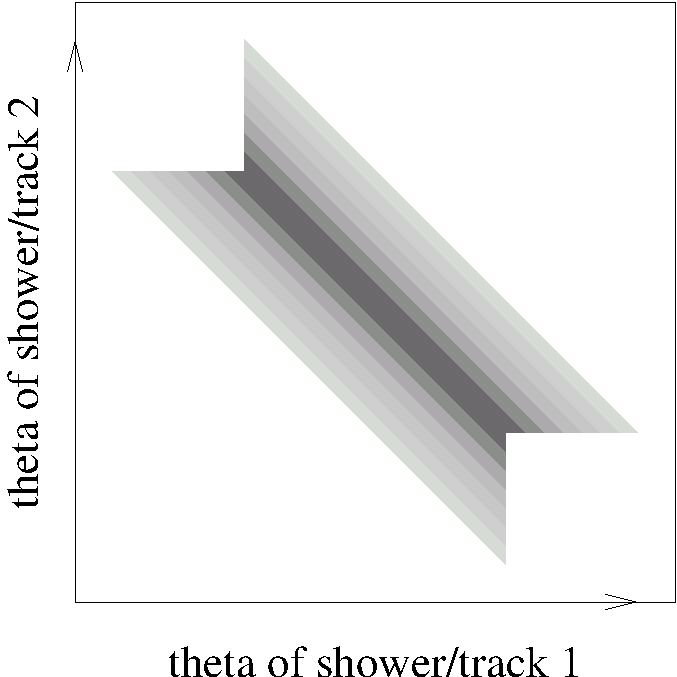
\includegraphics[width=0.4\linewidth]{plots/asymmetriccartoon}
  \end{center}
  \caption{\label{asymmetriccartoon} The distribution of two
  anti-correlated variables with an asymmetric cut such as the ones we
  applied to identify Bhabhas and \gamgam\ events.  Horizontal and
  vertical smearing around the central diagonal is independent; we cut
  each track or shower in a way that doesn't imply a cut on the
  other.}
\end{figure}

The Bhabha cuts we used are the same ones used for most other CLEO
luminosity measurements.  At an earlier stage in our analysis, we had
a different set of Bhabha cuts with a somewhat looser track momentum
threshold (70\%, rather than 90\% of \ecm).  All of the following
studies, including the final lineshape fits, are insensitive to our
choice of Bhabha cuts.

Contamination from $\Upsilon \to e^+e^-$ at the resonance peaks is
3\%, \bork\%, and \bork\%, respectively.  This background is readily
calculated for any \ecm\ by multiplying the \ups\ lineshape by \bee\
(we assume \bee\ = \bmm\ for greater precision) and the Bhabha cut
efficiency for $\Upsilon \to e^+e^-$ (which has a different angular
distribution than Bhabhas).  Since the \ups\ lineshapes are derived
from cross-section measurements, this is a circular dependence, so we
applied an iterative procedure, starting with \gamgam\ luminosity.
The \ups\ and continuum \ee\ interfere, so we also calculate an
interference term (Equation \ref{eqn:yint}) with $\alpha_\subs{int}$ =
\bork.  The effective cross-section for \ee\ as a function of \ecm,
including the continuum and \ups\ contributions, is presented in
Figure~\ref{allee}, with and without the interference term.  The
presence of the interference term has negligible impact on the
lineshape fit results.

\begin{figure}[p]
  \begin{center}
    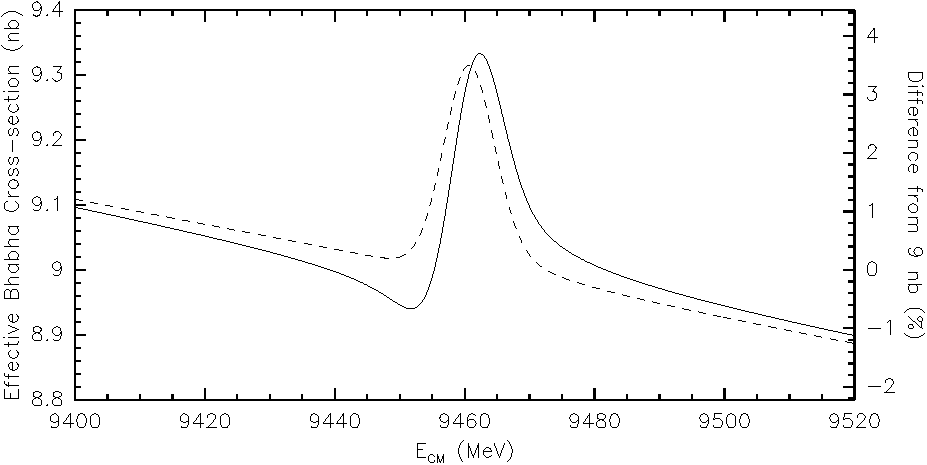
\includegraphics[width=\linewidth]{plots/allee}
  \end{center}
  \caption{\label{allee} The influence of $\Upsilon \to e^+e^-$ on
  effective \ee\ cross-section, with interference (solid) and without
  interference (dashed).  Note that the vertical axis is
  zero-suppressed.}
\end{figure}

A \gamgam\ event must have
\begin{itemize}

  \item two showers (subscripted 1 and 2) with energies higher than
    70\% of \ebeam,

  \item $|\cot\theta_1 + \cot\theta_2| < 0.1$ (showers back-to-back in
    $\theta$, the polar angle), and

  \item $|\sin(\phi_1 - \phi_2)| < 0.04$ (showers back-to-back in
    $\phi$, the azimuthal angle).

  \item The larger (smaller) $|\cot\theta|$ must be less than 1.28 (1.18)
    (this is within the calorimeter barrel),

  \item the larger (smaller) $|\cot\theta|$ must be greater than 0.15
  (0.05) (avoiding the central region, where trigger efficiency is
  low), and

  \item there must be no tracks in the event.

\end{itemize}
When we select \gamgam\ events, we are dependent on only one trigger,
\barrelbhabha, since this is the only trigger algorithm that doesn't
require any tracks.  We studied the efficiency of this trigger with
Bhabhas, and found calorimeter tiles whose efficiencies dropped for a
significant fraction of the data-taking period.  Rather than applying
a run-dependent efficiency, we masked out these regions with our cuts.
The largest shower on the western side of the detector must not be
found in any of these regions:
\begin{itemize}

  \item $-\frac{14}{64}\pi < \phi < \frac{9}{64}\pi$ and
    $|\cot\theta_1 + \cot\theta_2| < 1.08$,

  \item $-\frac{53}{64}\pi < \phi < -\frac{14}{64}\pi$ and
    $|\cot\theta_1 + \cot\theta_2| > 1.90$, and

  \item $-0.4 < \phi < -0.3$.

\end{itemize}
Given these angular cuts, the \barrelbhabha\ trigger is 99.67\%
efficient with only statistical deviations.  (The efficiency of every
run is above 99.2\%.)

\section{Overall Luminosity Scale}

The efficiency-weighted Bhabha cross-section is the second ingredient
in the luminosity measurement.  This sets the luminosity scale for all
Bhabha counts.  This scale factor, a number of nb\inv\ per observed
Bhabha, is the inverse of the efficiency-weighted Bhabha cross-section
(nb).

The efficiency-weighted cross-section is the cross-section of observed
Bhabhas.  Expressed as an integral over a single variable for clarity,
\begin{equation}
  \sigma_\subs{eff} = \int_0^\pi \frac{d\sigma}{d\theta} \,
  \epsilon(\theta) \, d\theta
  \label{eqn:effectivecrosssection}
\end{equation}
where $\epsilon(\theta)$ is our detector's Bhabha cut efficiency at a
given polar angle $\theta$.  Rather than exhaustively simulating the
detector's response to Bhabhas in $\theta$ bins, we generate Bhabhas
with an angular cut-off beyond the detector's geometric acceptance
(where $\epsilon(\theta) = 0$), calculate the efficiency-weighted cross-section
this represents ($\sigma_0$), and multiply it by the efficiency of
these simulated events ($\epsilon_0$), determined by passing them
through the detector simulation.  Both $\sigma_0$ and $\epsilon_0$
depend on our choice of cut-off, but the product doesn't.  This
product is the desired efficiency-weighted cross-section because
\begin{equation}
  \sigma_0 = \int_{\theta_\subs{min}}^{\theta_\subs{max}}
  \frac{d\sigma}{d\theta'} \, d\theta'
  \mbox{\hspace{0.5 cm} and \hspace{0.5 cm}}
  \epsilon_0 = \int_{\theta_\subs{min}}^{\theta_\subs{max}}
  \frac{dP}{d\theta} \, \epsilon(\theta) \, d\theta \mbox{.}
\end{equation}
where $dP/d\theta$ is the probability distribution of Bhabhas with
polar angle $\theta$ in our simulation, and $dP/d\theta$ is a
normalized differential cross-section
\begin{equation}
  \frac{dP}{d\theta} = \left(\frac{d\sigma}{d\theta}\right) \left(
  \int_{\theta_\subs{min}}^{\theta_\subs{max}}
  \frac{d\sigma}{d\theta'} \, d\theta' \right)^{-1}_{\mbox{\normalsize .}}
\end{equation}

We simulate Bhabhas with the Babayaga event generator, which
calculates differential cross-sections and $\sigma_0$ to fourth order
in the fine structure constant.  Our angular cut-off is
$|\cos\theta_\subs{max}|$ = \bork, and our initial-state radiation
cut-off is \bork\% of \ecm.  Passing these simulated events through
our full detector simulation, we calculate an efficiency-weighted cross-section
of 8.993 \PM\ 0.035 nb\inv\ at an \ecm\ of 9.43~GeV, 7.945 \PM\ 0.031
nb\inv\ at 10.00~GeV, and 7.361 \PM\ 0.032~nb\inv\ at 10.33~GeV, which
are the off-resonance \us, \uss, and \usss\ energies, respectively.

The Monte Carlo reproduces data distributions well at all three
energies, which is demonstrated for the 10.33~GeV data in eight
relevant distributions in
Figures~\mbox{\ref{eeagreementa}--\ref{eeagreementh}}.

\begin{figure}[p]
  \begin{center}
    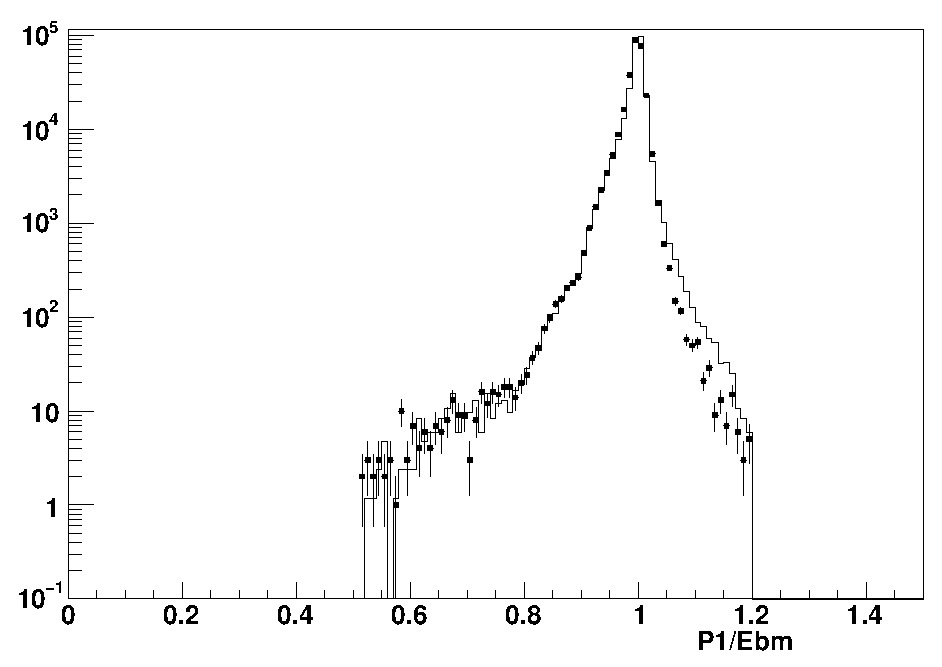
\includegraphics[width=0.7\linewidth]{plots/eeagreementb}
  \end{center}
  \caption{\label{eeagreementa} Largest track momentum divided by
  \ebeam\ in the 10.33~GeV data (points) and Monte Carlo (histogram)
  with other cuts applied.  Data between 0.5 and 1.1 are accepted.}
\end{figure}

\begin{figure}[p]
  \begin{center}
    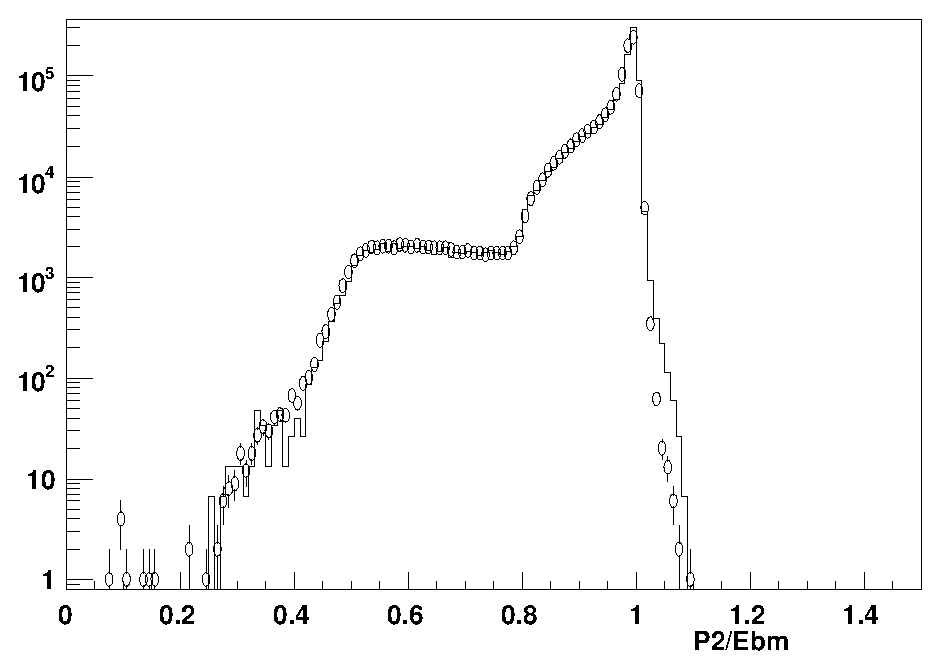
\includegraphics[width=0.7\linewidth]{plots/eeagreementc}
  \end{center}
  \caption{\label{eeagreementb} Second-largest track momentum divided
  by \ebeam\ in the 10.33~GeV data (points) and Monte Carlo
  (histogram) with other cuts applied.  Data between 0.5 and 1.1 are
  accepted.}
\end{figure}

\begin{figure}[p]
  \begin{center}
    \includegraphics[width=0.7\linewidth]{plots/eeagreementa}
  \end{center}
  \caption{\label{eeagreementc} Sum of two largest-momentum track
  energies and associated bremsstrahlung showers divided by \ecm\ in
  the 10.33~GeV data (points) and Monte Carlo (histogram) with other
  cuts applied.  Data above 0.9 are accepted.}
\end{figure}

\begin{figure}[p]
  \begin{center}
    \includegraphics[width=0.7\linewidth]{plots/eeagreementd}
  \end{center}
  \caption{\label{eeagreementd} Positron $\cos\theta$ (polar angle)
  distribution in the 10.33~GeV data (points) and Monte Carlo
  (histogram) with other cuts applied.  The larger (smaller)
  $|\cos\theta|$ of the two electrons must be below 0.766 (0.707) for
  acceptance.}
\end{figure}

\begin{figure}[p]
  \begin{center}
    \includegraphics[width=0.7\linewidth]{plots/eeagreementf}
  \end{center}
  \caption{\label{eeagreemente} Largest
  $E_\subs{shower}/|\vec{p}_\subs{track}|$ divided by \ebeam\ in the
  10.33~GeV data (points) and Monte Carlo (histogram) with other cuts
  applied.  Data above 0.8 are accepted.}
\end{figure}

\begin{figure}[p]
  \begin{center}
    \includegraphics[width=0.7\linewidth]{plots/eeagreementg}
  \end{center}
  \caption{\label{eeagreementf} Second-largest
  $E_\subs{shower}/|\vec{p}_\subs{track}|$ divided by \ebeam\ in the
  10.33~GeV data (points) and Monte Carlo (histogram) with other cuts
  applied.  Data above 0.5 are accepted.}
\end{figure}

\begin{figure}[p]
  \begin{center}
    \includegraphics[width=0.7\linewidth]{plots/eeagreemente}
  \end{center}
  \caption{\label{eeagreementg} Positron $\phi$ (azimuthal angle)
  distribution in the 10.33~GeV data (points) and Monte Carlo
  (histogram) with other cuts applied.  This variable is not used for
  cuts.}
\end{figure}

\begin{figure}[p]
  \begin{center}
    \includegraphics[width=0.7\linewidth]{plots/eeagreementh}
  \end{center}
  \caption{\label{eeagreementh} Number of charged tracks in the
  10.33~GeV data (points) and Monte Carlo (histogram) with other cuts
  applied.  This variable is not used for cuts.}
\end{figure}

The efficiency-weighted Bhabha cross-sections at 9.43, 10.00, and 10.33~GeV
differ by more than $1/s$ because the Monte Carlo finds these Bhabha
cuts to be energy-dependent.  We checked this claim by loosening the
cut on the energy sum of the two electrons from 90\% of \ecm\ to 70\%,
which removes the energy dependence.  We observed the same \bork\% per
GeV effect in data by re-imposing the tight cut.

We additionally determine the efficiency-weighted cross-sections of $e^+e^- \to
\mu^+\mu^-$ and $e^+e^- \to \gamma\gamma$ to reduce systematic
uncertainties by comparing the luminosity predicted for the same
dataset by different processes.  We follow \cite{oldlumi} to assign
1.6\% systematic uncertainties for Bhabha efficiency-weighted cross-section,
1.6\% for \mumu, and 1.8\% for \gamgam.  The sources of these
uncertainties are tabulated in Table~\ref{tab:lumisyst}: \ee\ and
\mumu\ uncertainties are dominated by the degree of resonance
interference and the track-finding efficiency, while \gamgam\
uncertainties are dominated by the photon-finding efficiency and
angular resolution.

\begin{table}
  \caption{\label{tab:lumisyst} Fractional systematic uncertainties in
  our determinations of the efficiency-weighted cross-sections of \ee, \mumu,
  and \gamgam.  All values are percentages.}
  \begin{center}
    \begin{tabular}{p{0.5\linewidth} | c c c}
      \hline\hline
      & \ee & \mumu & \gamgam \\\hline
      Finite Monte Carlo sample & 0.4 & 0.5 & 0.6 \\
      Radiative corrections & 0.5 & 0.5 & 0.5 \\
      Resonance interference & 1.0 & 1.0 & \\
      Trigger efficiency & 0.1 & 0.1 & 0.7 \\
      Track-finding efficiency & 1.0 & 1.0 & \\
      Photon-finding efficiency & & & 1.0 \\
      Dependence on cuts & 0.5 & 0.3 & 1.0 \\
      Cosmic ray backgrounds & & 0.2 & \\
      ISR tail backgrounds & & 0.1 & \\\hline
      Total & 1.6 & 1.6 & 1.8 \\\hline\hline
    \end{tabular}
  \end{center}
\end{table}

We can compare these as luminosity measurements by dividing the \ee,
\mumu, and \gamgam\ counts from the same sample--- all available
off-resonance data--- by their efficiency-weighted cross-sections.  We obtain
the integrated luminosities plotted in Figure~\ref{comparelumis},
which are in good agreement, considering their systematic
uncertainties.  The \ee\ and \mumu\ modes share the same track-finding
efficiency, so we draw error bars with this systematic removed in the
Figure.

\begin{figure}[p]
  \begin{center}
    \includegraphics[width=\linewidth]{plots/comparelumis}
  \end{center}
  \caption{\label{comparelumis} The integrated luminosity of all
  off-resonance data combined, as determined from \ee, \mumu, and
  \gamgam\ counts.  Outermost errorbars include all systematic
  uncertainties, and the second errorbars on \ee\ and \mumu\ have
  common tracking and resonance interference systematics removed.
  Innermost errorbars (visible only for \mumu) are statistical-only.
  The weighted average and RMS of the three measurements are
  represented by dashed and dotted horizontal lines.}
\end{figure}

The average luminosity from \ee, \mumu, and \gamgam\ is only
0.2--0.6\% higher than the \ee\ luminosity alone (depending on
dataset), so we modify our luminosity determination to return the
average luminosity from the three processes.  The integrated
luminosity is 0.1114~nb\inv, 0.1266~nb\inv, and 0.1361~nb\inv\ per
observed Bhabha event in the 9.43, 10.00, and 10.33~GeV datasets,
respectively.  We call these the luminosity scale factors.

Without knowing that \mumu\ and \gamgam\ measurements reproduce the
Bhabha result, we would have a 1.6\% uncertainty common to all three
luminosity scale factors.  However, we can incorporate this
information by assigning the \ee, \mumu, and \gamgam\ RMS differences
from the average as the common uncertainty.  Thus, the luminosity
scale factors have an uncertainty of 1.3\%.  \label{sec:luminosity}
The luminosity scale factor is a factor in \geehadtot, so the
fractional uncertainty in this scale factor adds to the \geehadtot\
fractional uncertainty in quadrature.

[re-write, needs more intro] One could determine \gee$(nS)$/\gee$(mS)$
without knowing the integrated luminosity of any dataset, using only
Bhabha event counts to compare relative luminosities.  Thus,
uncertainties in the luminosity scale factors for the 9.43, 10.00, and
10.33~GeV datasets are highly correlated.  To relate integrated
luminosities near the $\Upsilon(nS)$ with integrated luminosities near
the $\Upsilon(mS)$, one only needs to know the relative Bhabha
efficiencies at the two center-of-mass energies.  We determined this
with Monte Carlo simulations which are limited only by their finite
sample sizes.  This implies a 0.5\% uncertainty in the ratios of
integrated luminosities of different resonances.

To blind our analysis, we determined the overall luminoisty scale
factors last, after all background (Chapter \ref{chp:backgrounds}),
efficiency (Chapter \ref{chp:efficiency}), and beam energy studies
(Chapter \ref{chp:beamenergy}) were completed.  Until that point, we
only knew the relative luminosities of our data samples, and therefore
only relative cross-sections.  We incorporated these scale factors
(using \gamgam\ event counts, rather than Bhabha event counts) just
before presenting preliminary \gee\ results at the European Physical
Society meeting in July, 2005.

\section{Consistency of Bhabhas with \boldmath \gamgam}

Above, we took advantage of the \gamgam\ luminosity measurement's very
different systematic uncertainties to check and correct the Bhabha
scale factors off-resonance, but we have not yet used the fact that
\gamgam\ counts are unaffected by \ups\ decays.  In this Section, we
will compare Bhabha and \gamgam\ rates as a function of \ecm\ through
the \ups\ resonances, to test the $\Upsilon \to e^+e^-$ correction.
We tune the \gamgam\ luminosity measurement to yield the same results
as Bhabhas off-resonance and measure the \gamgam\ and Bhabha
luminosities in \ups\ data.  Both methods should yield the same
integrated luminosity, within statistical uncertainties.

\label{sec:luminosityconsistency}
[Turn all these numbers into plots; note the larger data samples at
peak] We find instead that \gamgam\ luminosity is (0.8 \PM\ 0.2)\%
higher on the \us, (0.3 \PM\ 0.4)\% higher on \uss, and (0.7 \PM\
0.2)\% higher on \usss, if we combine all scan and peak data.  This
result is unchanged if we restrict our test to data within 0.8~MeV of
the peak of each resonance.  If we consider other subsets of the \ups\
data, we do not have the statistical significance to see this
discrepancy.  The direction of this effect could be explained by an
$\Upsilon \to e^+e^-$ over-subtraction, but not the magnitudes.  The
\us\ and \usss\ peak cross-sections are 18~nb and 4~nb, respectively,
with the same \bee, so one would expect an over-subtraction to be 4.5
times as severe in the \us\ case than the \usss.  Instead, they appear
to be nearly equal.  Even accounting for their large fractional
uncertainties, a factor of 4.5 is disfavored by more than two standard
deviations.  The discrepancy is also \bork\ times too large to be
explained by \ecm\ dependence in the Bhabha cut efficiency.
(Integrated luminosity is in the denominator of cross-section, and
\geehadtot\ is proportional to cross-section.)

We do not know whether the discrepancy is due to an error in the
Bhabha measurement or in the \gamgam\ measurement, so we apply half of
this discrepancy as a correction and add half the discrepancy and its
uncertainty in quadrature to the total uncertainty in luminosity, to
cover the ambiguity.  This is only a 0.4\% uncertainty in the
luminosity of each resonance, and therefore a small contributor to the
total \gee\ uncertainty.

[Re-write] As a cross-check, we also selected Bhabhas in two disjoint
angular regions: inner ($0 < \cos\theta_+ < 0.6$) and outer ($0.6 <
\cos\theta_+ < 0.8$, where $\theta_+$ is the polar angle of the
positron--- Bhabha cross-section diverges at $\cos\theta_+ = 1$).  The
inner Bhabhas have a greater fractional contamination from \ups\ than
the outer Bhabhas, as well as a larger interference term, but \ups\
fit results are consistent when using inner, outer, and all Bhabhas.

\chapter{Beam Energy Measurement}
\label{chp:beamenergy}

Having presented all the details necessary to properly measure the
hadronic \ups\ cross-section, the vertical axis in our lineshape plot
(Figure~\ref{cartoon}), we now consider our measurement of \ecm, the
horizontal axis.  In Chapter \ref{chp:hardware}, we discussed the
mechanism which determines the beam energy of each run.  While this
reckoning differs from the true beam energy by 8~MeV near the \ups\
resonances [how do we know?], we will show in this Chapter that measurements of beam
energy differences are robust enough for the precision demands of this
analysis.

The masses of the \ups\ resonances have been measured with
0.3--0.5~MeV precision at Novosibirsk, so we can use the \ups\
lineshapes as calibrating markers in beam energy.  If we correct our
\ecm\ measurements by a constant shift [not scale factor?] at the \us,
we almost reproduce the Novosibirsk \uss\ and \usss\ masses: our
average \uss\ mass is 0.65 \PM\ 0.18~MeV too low, and our average
\usss\ mass is 1.60 \PM\ 0.30~MeV too low
(Figure~\ref{energycalibration}).  If this error is purely a function
of beam energy and is not related to alterations in CESR's
configuration between the \usss, \us, and \uss\ data-taking periods,
then our beam energy measurements differ from the true beam energies
by a linear transformation, which we determine with a fit to the three
apparent \ups\ masses in Figure~\ref{energycalibration}.  If this
tranformation applies to small changes in beam energy (scan point
differences, about 10~MeV) as well as large (300~MeV between
resonances), the resonance scans are too narrow, and \geehadtot\ is
too low, by only 0.2\%.  We do not apply this as a correction.

\begin{figure}[p]
  \begin{center}
    \includegraphics[width=\linewidth]{plots/energycalibration}
  \end{center}
  \caption{\label{energycalibration} Difference between the measured
  mass and the true mass of the \us, \uss, and \usss, where the \us\
  measurement has been shifted to the true mass.  Outer errorbars
  represent the RMS of all scan measurements, inner errorbars are
  statistical-only.  The dashed curve is a fit.}
\end{figure}

Potentially more worrisome are variations in the beam energy with
time.  The measurement of beam energy differences is very sensitive to
the placement of the NMR probes in the test magnets, because at the
0.05\% level (corresponding to 1~MeV in \ecm), the magnetic field in
the test magnets is a function of position.  Every week, these probes
are exposed to the possibility of movement as a consequence of CESR
machine studies [how?].  To protect our lineshape scans from discrete
shifts in beam energy calibration, we divided our data-taking into
short, independent 10-hour scans, plus 38~hours of subsequent peak
running, separated by about a week.  The test magnets were not
disturbed during these dedicated scans or during the peak data-taking
associated with each scan.  Changes in the apparent \ups\ mass from
one week to the next alert us to shifts in the beam energy measurement
between scans, which we observe as a slow drift on the order of
0.5~MeV per month (Figure~\ref{beamenergydrift}).  To be insensitive
to these drifts, we include the apparent \ups\ mass of each 10+38-hour
scan as an independent parameter in the lineshape fit.  Values of
\ecm\ in the lineshape fit are only relative to the apparent \ups\
mass from the week the data were taken.

\begin{figure}[p]
  \begin{center}
    \includegraphics[width=\linewidth]{plots/beamenergydrift}
  \end{center}
  \caption{\label{beamenergydrift} Difference between the measured
  mass and the true mass of the \us, \uss, and the \usss\ (top to
  bottom), for each individual scan.  Dashed horizontal lines
  represent the weighted averages.}
\end{figure}

We are only sensitive to random changes in beam energy, or jitter, on
a 10-hour timescale.  We have already ensured our insensitivity
to week-by-week fluctuations.  If the beam energy fluctuates on very
short timescales, much less than an hour (the length of a run), then
the jitter only contributes to beam energy spread.  (In this
sense, the beam energy fluctuates by about 4~MeV with every
collision!)  We reduce sensitivity to monotonic 10-hour drifts by
alternating scan points above and below the \ups\ peak, so that a
drift would not systematically widen or narrow the lineshape.

To check for changes in the beam energy calibration on the
10-hour timescale, we measure the cross-section at a high-derivative
point on the lineshape twice, usually at the beginning and end of a
scan.  Since the derivative is high, significantly different
cross-section results at the same reported beam energy would be an
indication that the actual beam energy has shifted between the two
measurements.  Any cross-section difference ($\sigma_1-\sigma_2$) can
be converted into a true beam energy difference ($E_1-E_2$) at a given
lineshape derivative ($\sigma'(E)$) by
\begin{equation}
  \borkborkbork \mbox{.}
\end{equation}
To find possible shifts in calibration, we subtract the true beam
energy difference from the reported difference, and propagate
uncertainties from the cross-section measurement.  We call this a
shift ($s_i \pm \delta_{s_i}$).  All shifts are consistent with zero
[quantify].  We plot these shifts with their uncertainties in
Figure~\ref{miscalhours}.  As there is no evidence for any calibration
shift, we construct a 68\% confidence level upper limit on the typical
10-hour jitter, $j$, by calculating the $j$ necessary to lower the
total log-likelihood of our repeated measurements by 1/2.
Log-likelihood is defined as
\begin{equation}
  L(j) = \sum_{i=1}^{29} \ln \left(
  \frac{1}{\sqrt{2\pi({\delta_{s_i}}^2 + j^2)}} \exp\left(\frac{-{s_i}^2}{2
  ({\delta_{s_i}}^2 + j^2)} \right) \right)
\end{equation}
Only jitters larger than 0.05~MeV are inconsistent with the data.  An
alternate method, analogous to the PDG's $S$-factor, sets the upper
limit at 0.07~MeV.  As a fraction of the total beam energy, this is
5--7 parts per million.

\begin{figure}[p]
  \begin{center}
    \includegraphics[width=\linewidth]{plots/miscalhours}
  \end{center}
  \caption{\label{miscalhours} Beam energy shifts ($s_i$) determined
  by pairs of repeated cross-section measurements, plotted with
  respect to the time between the first and the second measurement.
  The weighted mean of $\{s_i\}$ is 0.02 \PM\ 0.03~MeV, so the apparent
  vertical asymmetry of this distribution is an illusion.}
\end{figure}

\begin{figure}[p]
  \begin{center}
    \includegraphics[width=\linewidth]{newplots/energylj}
  \end{center}
  \caption{\label{energylj} Log-likelihood ($L(j)$) as a function of
  jitter ($j$) attains a maximum near $j=0$ and is reduced by 1/2 at
  $j=0.05$~MeV.}
\end{figure}

To learn what fluctuations of this size imply for uncertainty in
\geehadtot, we simulated the lineshape fits with random perturbations
in the measured beam energy.  The nominal \ecm\ and luminosity of each
simulated cross-section measurement were copied from the real data
sample, but the cross-sections themselves were derived from an ideal
curve with statistical errors.  Without perturbing the simulated beam
energy measurements, the fits return our input \geehadtot\ with
perfectly-distributed $\chi^2$ values.  When \ecm\ is randomly
perturbed with a standard deviation of 0.07~MeV, the value of
\geehadtot\ fluctuates up and down by 0.2\% of itself, and the
$\chi^2$ increases by only \bork, \bork, and \bork\ for the \us, \uss,
and \usss.  \label{pag:notjitter} We therefore assign a 0.2\%
systematic uncertainty in \geehadtot\ and \gee\ due to the possibility
of beam energy measurement errors.

\chapter{Lineshape Fitting}
\label{chp:fitting}

This is the core of the analysis: all previous studies were meant to
determine the placement of data and the shape of the function for this
fit.  In this Chapter, we will review the fit function and all of its
parameters, present the fit and the fit results, and discuss how
hadron-level interference can potentially affect the fit results by as
much as 1\%.

\section{The Fit Function}
\label{sec:fitfunction}

As a single expression, the fit function for the $\Upsilon(nS)$
lineshape is the following:
\begin{multline}
  \sigma_n(E_\subs{CM}) = \epsilon_\subs{had} \, \sigma_\subs{had}(E_\subs{CM}) +
  \epsilon_{\tau\tau} \, {\mathcal B}_{\tau\tau} \, \sigma_{\tau\tau}(E_\subs{CM}) +
  \sigma_{n-1}(E_\subs{CM}) \\
  + \sigma_\subs{cont} \left((1-f) \frac{\mbox{9 GeV}}{{E_\subs{CM}}^2}
  + f \log\left(\frac{{E_\subs{CM}}^2}{\mbox{9 GeV}}\right)\right) \mbox{,}
  \label{eqn:fitfunc}
\end{multline}
where $\sigma_{n-1}(E_\subs{CM})$ is the previously-fitted lineshape
of the $\Upsilon((n-1)S)$ (non-existent for \us), and
$\sigma_\subs{had}(E_\subs{CM})$ and $\sigma_{\tau\tau}(E_\subs{CM})$
are both three-way convolutions in \ecm.
\begin{multline}
  \sigma_\subs{had/\tautau}(E_\subs{CM}) = BW(E_\subs{CM}', A, M_1, \ldots M_N, \Gamma,
  \alpha_\subs{int}, \phi_0) \\ \otimes \, G(E_\subs{CM}'', \Delta E_1, \ldots \Delta E_N)
  \, \otimes \, \mbox{ISR}(E_\subs{CM}''') \mbox{.}
\end{multline}
The $BW$ function is a Breit-Wigner with interference---
$(\sigma_\subs{res}+\tilde{\sigma}_\subs{int})$ from Equation
\ref{eqn:rescontinter}.  A description of each argument of
$\sigma_\subs{had/\tautau}(E_\subs{CM})$ follows.
\begin{description}

  \item[\boldmath $A$] is the area of the Breit-Wigner, that is, $\int \sigma(e^+e^-
    \to \Upsilon \to \mbox{hadronic}) \, dE_\subs{CM}'$ for Equation
    \ref{eqn:gee} and the goal of this entire analysis.

  \item[\boldmath $M_1, \ldots M_N$] is the apparent \ups\ mass in each 10+38-hour
    scan, as discussed in Chapter~\ref{chp:beamenergy}.

  \item[\boldmath $\Gamma$] is the full width of the \ups\ resonance.
    Our fits are sensitive to $\Gamma$ only at the 0.03\% level, so we
    use previously-measured values, which are consistent with the
    values we determine from the fits.

  \item[\boldmath $\alpha_\subs{int}$ and $\phi_0$] are continuum
    interference parameters, defined by Equation \ref{eqn:yint}.  We
    assume that only the $\Upsilon \to q\bar{q}$ decays interfere with
    continuum \qqbar.  Uncertainties in \geehadtot\ due to the
    hadronic $\alpha_\subs{int}$ are 0.02\%, and uncertainties due to the
    \tautau\ $\alpha_\subs{int}$ are 0.08\%.  We will discuss another
    source of interference, which can potentially modify $\phi_0$, in
    Section \ref{sec:interference} below.

\end{description}
The second function in the convolution is a unit Gaussian to describe
the beam energy spread, with different values of the beam energy
spread $\Delta E_i$ for run ranges with potentially different beam
energy spreads, as described on page \pageref{pag:beamenergyspread} in
Section \ref{pag:beamenergyspread}.  The ISR function, calculated from
perturbative QED by Kuraev and Fadin \cite{kf}, Equation (28), has no
free parameters.  The normalization of the observed tail is inherited
from the Breit-Wigner area, through the convolution.  The 0.1\%
theoretical uncertainty in ISR normalization propagates to a 0.05\%
uncertainty in \geehadtot.  The hadronic ($\sigma_\subs{had}$) and
\tautau\ ($\sigma_{\tau\tau}$) lineshapes have the same values for all
parameters except $\alpha_\subs{int}$.

The fit function includes the following constants in addition to
$\Gamma$, $\alpha_\subs{int}$, and $\phi_0$.
\begin{description}

  \item[\boldmath $\epsilon_\subs{had}$] is the hadronic \ups\
    efficiency, measured for \us, \uss, and \usss\ in Chapter
    \ref{chp:efficiency}.  We apply this correction to the fit
    function, rather than the data.

  \item[\boldmath $\epsilon_{\tau\tau}$] is the \tautau\ efficiency,
    determined from Monte Carlo in Chapter \ref{chp:backgrounds}.

  \item[\boldmath ${\mathcal B}_{\tau\tau}$] is the \tautau\ branching
    fraction used to subtract \tautau\ backgrounds.

    As explained in Chapter \ref{chp:technique}, we fit hadronic
    cross-sections to obtain \geehadtot\ without assuming Lepton
    Universality, and then divide by $(1-3{\mathcal B}_{\mu\mu})$ to
    reintroduce the leptonic modes for \gee.  In Chapter
    \ref{chp:backgrounds}, we saw $\Upsilon \to \tau^+\tau^-$ as a
    background.  When we derive \gee, we subtract the \tautau\ that
    survives our cuts to determine \geehadtot, and then add all the
    \tautau\ back in, along with \ee\ and \mumu, to determine \gee.
    For \gee, we want to use the same branching fraction for both
    operations, so we derive \gee\ from fits that use \bmm\
    \cite{istvan} to estimate the \tautau\ background, and derive
    \geehadtot\ from fits that use the most precise \btt\ available,
    from \cite{jean}.

    Even the larger uncertainty in \btt\ affects fit results by less
    than 0.1\%, and $\epsilon_{\tau\tau}$ fractional uncertainties are
    smaller yet, so the systematic errors introduced by
    $\epsilon_{\tau\tau}$ and \btt\ are both negligible.

[Note to self: ${\mathcal B}_{\tau\tau}$ in equation \ref{eqn:fitfunc}
really ought to have been ${\mathcal
B}_{\tau\tau}\Gamma_\subs{had}/\Gamma_\subs{tot}$.  This makes my
quoted \geehadtot\ and \gee\ 0.1\% too small.]

  \item[\boldmath $f$] is the fraction of the continuum which scales
    as $\log s$, rather than $1/s$, at 9~GeV.  This was determined by
    a fit to the three off-resonance cross-sections in Section
    \ref{pag:logs} on page \pageref{pag:logs}.  The uncertainty this
    parameter imposes on \geehadtot\ is 0.002\%.

\end{description}

The \us\ fit has a total of sixteen floating parameters: $A$, $M_1,
\ldots M_{11}$ for its eleven 10+38-hour scans, $\Delta E_1, \Delta E_2,
\Delta E_3$ for the three groups of 10+38-hour scans with potentially
different beam energy spreads, and $\sigma_\subs{cont}$, the continuum
level at 9~GeV.  The \uss\ fit has nine floating parameters: $A$,
$M_1, \ldots M_6$ for its six 10+38-hour scans, a single beam energy
spread $\Delta E$ (the CESR beam energy spread was stable), and
$\sigma_\subs{cont}$.  The \usss\ fit has sixteen floating parameters:
$A$, $M_1, \ldots M_7$ for its seven 10+38-hour scans, $\Delta E_1,
\ldots \Delta E_7$ for all seven scans, and $\sigma_\subs{cont}$.

\section{Fit Results}

We used a {\tt C++} version of {\tt MINUIT} from the {\tt SEAL}
package to perform a $\chi^2$ fit of our lineshape data to Equation
\ref{eqn:fitfunc}.  The resulting best-fit values for $A$ are listed
in Table~\ref{tab:bestfit}.  The best-fit functions are plotted in
Figure~\ref{fitresults}, overlaying data.  Also plotted in this Figure
are pull distributions for the data, where pull is the ratio of
residual to uncertainty, highlighting the significance of deviations
from the best-fit line.  More detailed pull distributions are plotted
in Figures~\ref{pullsone}, \ref{pullstwo}, and \ref{pullsthree}, for
the \us, \uss, and \usss, respectively.  All data points are visible
in these plots: no points have pulls larger than 3.5.

\begin{table}
  \caption{\label{tab:bestfit} Best-fit $A$ and $\chi^2$ significance.}
  \begin{center}
    \begin{tabular}{c c c c c}
      \hline\hline
      & $A$ & reduced $\chi^2$ & & confidence level \\\hline
      \us & \bork\ MeV nb & \bork/(\bork - \bork) = & \bork & \bork\% \\
      \uss & \bork\ MeV nb & \bork/(\bork - \bork) = & \bork & \bork\% \\
      \usss & \bork\ MeV nb & \bork/(\bork - \bork) = & \bork & \bork\% \\\hline\hline
    \end{tabular}
  \end{center}
\end{table}
    
\begin{figure}[p]
  \begin{center}
    \includegraphics[width=\linewidth]{plots/fitresults}
  \end{center}
  \caption{\label{fitresults} Best-fit lineshapes (solid) to the \us,
  \uss, and \usss\ data (points), from which \geehadtot\ is
  determined.  Dashed curves are total background estimates, and the
  pull distributions above each plot indicate the statistical
  significance of all deviations from the best-fit line.  Insets for
  each resonance present a tail measurement \bork--100~MeV above the
  \ups\ masses.}
\end{figure}

\begin{figure}[p]
  \begin{center}
    \includegraphics[width=\linewidth]{plots/pullsone}
  \end{center}
  \caption{\label{pullsone} The pull distribution of \us\ lineshape
  fits (a) as a function of \ecm, (b) as a function of date, and (c),
  as a histogram, fitted to a Gaussian curve, which is almost two
  standard deviations wider than unity.}
\end{figure}

\begin{figure}[p]
  \begin{center}
    \includegraphics[width=\linewidth]{plots/pullstwo}
  \end{center}
  \caption{\label{pullstwo} The pull distribution of \uss\ lineshape
  fits (a) as a function of \ecm, (b) as a function of date, and (c),
  as a histogram, fitted to a Gaussian curve, which is almost two
  standard deviations wider than unity.}
\end{figure}

\begin{figure}[p]
  \begin{center}
    \includegraphics[width=\linewidth]{plots/pullsthree}
  \end{center}
  \caption{\label{pullsthree} The pull distribution of \usss\
  lineshape fits (a) as a function of \ecm, (b) as a function of date,
  and (c), as a histogram, fitted to a Gaussian curve, which is
  statistically consistent with unity.}
\end{figure}

This fit function describes our data well: no trends are evident in
pull versus energy, but the \us\ and especially the \uss\ pull
distributions are wider than would be expected from statistical
fluctuations.  Equivalently, the $\chi^2$ per degree of freedom
($N_\subs{dof}$) is high, as can be seen in Table~\ref{tab:bestfit}.
In the \uss\ data, the high-energy tail is the largest deviation,
contributing 9.1 units to the total $\chi^2$, but this is only a fifth
of the excess.  (Dropping this point changes the \uss\ \geehadtot\ by
0.4\%.)  The jittering beam energy simulations, described at the end
of Section \ref{pag:notjitter} (page \pageref{pag:notjitter}),
demonstrate that uncertainty in beam energy can only account for
\bork\ units of $\chi^2$.  If the real beam energy spread deviated
from a pure Gaussian distribution, we would see trends in pull versus
\ecm.  We do not see such trends at this level of precision, and
therefore have no evidence that the CESR beam energy spread is
anything but a pure Gaussian.

These larger-than-expected deviations are symmetric around the
best-fit line at all \ecm\ and dates, and they do not favor a
particular \ecm\ or date (Figures~\ref{pullsone}--\ref{pullsthree}),
so we treat them as though we had underestimated our statistical
uncertainty ($\sigma_\subs{stat}$).  We add $\sigma_\subs{stat}
\sqrt{\chi^2/N_\subs{dof} - 1}$ to our systematic uncertainty in
\label{sec:chichiconsistency} quadrature, which has the same effect on
the total uncertainty as if we had multiplied $\sigma_\subs{stat}$ by
$\sqrt{\chi^2/N_\subs{dof}}$.

\section{Interference Between \boldmath \ggg\ and \qqbar}
\label{sec:interference}

In constructing a fit function, we assumed that continuum and \ups\
decays only interfere at the parton level, and not at the hadron
level.  That is, we assume that $e^+e^- \to q\bar{q}$ can interfere
with $e^+e^- \to \Upsilon \to q\bar{q}$ but not $e^+e^- \to \Upsilon
\to ggg$, even though both \qqbar\ and \ggg\ hadronize into some of
the same final states.  The \us\ fit favors this scheme over the
no-interference hypothesis by 3.7 standard deviations.  In fact,
assuming a \qqbar-like phase, the \us\ fit is optimized by \qqbar-only
interference, as can be seen in Figure~\ref{simpleintfit}.  However,
it is possible that interference between $e^+e^- \to q\bar{q} \to$
hadrons and $e^+e^- \to \Upsilon \to ggg \to$ hadrons is significant.
In this case, the resonance (at $E_\subs{CM} \ll M_\Upsilon$) minus
continuum phase difference, $\phi_0$, need not be zero, and our fit is
less well constrained.  This is a fundamental and interesting question
about the quantum mechanics of hadronization, and unfortunately our
data cannot answer this question for all phases.  It is also
unfortunate that some of the allowed hypotheses can modify \geehadtot\
by as much as \bork\%.

\begin{figure}[p]
  \begin{center}
    \includegraphics[width=0.8\linewidth]{plots/simpleintfit}
  \end{center}
  \caption{\label{simpleintfit} A fit of the \us\ for the magnitude of
  hadronic interference ($\alpha_\subs{int}$), assuming $\phi_0 = 0$.  The
  points are \us\ fits with trial $\alpha_\subs{int}$ values, the vertical
  axis is the $\chi^2$ of these fits, and the solid line is a parabola
  drawn through the points.  Dashed and dotted lines indicate the
  minimum and 68\% confidence level bands, and the circled point
  represents the nominal \qqbar-only fit we used in this anaysis.}
\end{figure}

The size of this shift is critically dependent on the phase difference
between $\Upsilon \to ggg \to$ hadrons and $\Upsilon \to q\bar{q} \to$
hadrons.  In Equation \ref{eqn:yint}, we see that if the total
$\phi_0$ is $\pm\pi/2$, the interference term ($\tilde{\sigma}_\subs{int}$)
has the same \ecm\ dependence as the resonance term
($\sigma_\subs{res}$).  The magnitude of $\tilde{\sigma}_\subs{int}$ and
$\sigma_\subs{res}$ would then be correlated or anticorrelated
(depending on sign), so interference uncertainty would add directly to
\geehadtot\ uncertainty.

To parameterize the effect of this unknown interference on \geehadtot,
we assume that all $\Upsilon \to q\bar{q}$ and a fraction of the
$\Upsilon \to ggg$ amplitude ($f_{ggg}$) interferes with continuum
\qqbar.  The phase difference between resonance and continuum \qqbar\
is known and is a function of \ecm, but the resonance \ggg\ minus
resonance \qqbar\ phase ($\phi_{ggg}$) is an unknown constant.  We fit
\us\ with a large set of $(f_{ggg}, \phi_{ggg})$ hypotheses to obtain
the following empirical parameterization:
\begin{equation}
  \Delta(\Gamma_{ee}\Gamma_\subs{had}/\Gamma_\subs{tot}) = -1.77\% \left(\frac{y_\subs{ggg}}{y_{q\bar{q}}} \sin(\phi_{ggg} + 0.3) \right)
  + 0.045\% \left(\frac{y_\subs{ggg}}{y_{q\bar{q}}} + 0.3 \left(\frac{y_\subs{ggg}}{y_{q\bar{q}}}\right)^2 \right)
  \label{eqn:areashift}
\end{equation}
where $y_\subs{ggg}/y_{q\bar{q}} = f_{ggg}\sqrt{{\mathcal
B}_{ggg}/{\mathcal B}_{q\bar{q}}}$.  Corrections for the \uss\ are
70\% as large as this and corrections for the \usss\ are 65\% as
large.

We cannot use exclusive processes such as $\pi^+\pi^-$ or $K^+K^-$ to
identify $\phi_0$ because these represent a small fraction of the
\qqbar\ and \ggg\ final states, and each exclusive mode may have a
different phase.  In fact, one argument for expecting a small
interference between \qqbar and \ggg\ decays relies on the very large
number of exclusive final states and the assumption that each has a
generic phase angle, thereby nearly cancelling in the sum.  In this
Section, we will treat the phase of the inclusive interference as
unknown.

Some constraints can be placed on the magnitude of \ggg\ interference
because $f_{ggg}$ is a measure of the overlap of \ggg\ and \qqbar\
final state wavefunctions.  [isospin and flavor arguments, which I
need to re-read and understand more quantitatively.  Just re-read
them: now I understand.  I'll give some thought to presentation before
proceeding.]

The \us\ fits provide another constraint which is tight for some
values of $\phi_{ggg}$.  When the total $\phi_0$ is far from
$\pm\pi/2$ and interference modifies the shape of the fit function,
large $f_{ggg}$ hypotheses inflate the best-fit $\chi^2$.  Figure~\ref{intconstraint} presents the 68\% confidence level upper limit on
$f_{ggg}$ as a function of $\phi_{ggg}$.  (The $\chi^2$ minimum is
always close to $f_{ggg} = 0$.)  Applying Equation \ref{eqn:areashift}
to this upper limit, we obtain an upper limit on \geehadtot\
corrections as a function of $\phi_{ggg}$ (Figure~\ref{areaconstraint}).

\begin{figure}[p]
  \begin{center}
    \includegraphics[width=0.8\linewidth]{plots/intconstraint}
  \end{center}
  \caption{\label{intconstraint} The fraction of \ggg\ amplitude
  allowed to interfere with continuum \qqbar\ ($f_{ggg}$), according
  to the \us\ fit at 68\% confidence level.  We have no sensitivity to
  this parameter if the \ggg\ minus \qqbar\ phase difference in \ups\
  decays ($\phi_{ggg}$) is near $\pm\pi/2$.}
\end{figure}

\begin{figure}[p]
  \begin{center}
    \includegraphics[width=0.8\linewidth]{plots/areaconstraint}
  \end{center}
  \caption{\label{areaconstraint} The possible correction to
  \geehadtot\ implied by our ignorance of $f_{ggg}$ at 68\% confidence
  level (gray) as a function of $\phi_{ggg}$.  The dashed lines
  represent upper limits including isospin and flavor arguments.}
\end{figure}

Our ignorance of \ggg/\qqbar\ interference implies at most a \bork\%
error in \geehadtot\ and \gee.  We do not assign a systematic
uncertainty for this effect because it is not related to the details
of our detector, and because its existence is disputed.  Though a
large inclusive interference between \qqbar\ and \ggg\ is a logical
possibility, it is not widely believed to be likely.

\chapter{Results and Conclusions}
\label{chp:results}

Our values of \geehadtot, quoted with statistical uncertainties
first and systematic uncertainties second, are
\begin{eqnarray}
  (\Gamma_{ee}\Gamma_\subs{had}/\Gamma_\subs{tot})(1S) &=& 1.252 \pm 0.004 \pm 0.019 \mbox{ keV,} \\
  (\Gamma_{ee}\Gamma_\subs{had}/\Gamma_\subs{tot})(2S) &=& 0.581 \pm 0.004 \pm 0.009 \mbox{ keV, and} \\
  (\Gamma_{ee}\Gamma_\subs{had}/\Gamma_\subs{tot})(3S) &=& 0.413 \pm 0.004 \pm 0.006 \mbox{ keV.}
\end{eqnarray}
Dividing by $(1-3{\mathcal B}_{\mu\mu})$, we obtain \gee:
\begin{eqnarray}
  (\Gamma_{ee})(1S) &=& 1.354 \pm 0.004 \pm 0.020 \mbox{ keV,} \\
  (\Gamma_{ee})(2S) &=& 0.619 \pm 0.004 \pm 0.010 \mbox{ keV, and} \\
  (\Gamma_{ee})(3S) &=& 0.446 \pm 0.004 \pm 0.007 \mbox{ keV.}
\end{eqnarray}
The total uncertainties for each resonance is less than 2\%.  Figure~\ref{historyplot} compares our \geehadtot\ to all previous
measurements: we find it to be consistent with, but more precise than,
the world average.  Note that \usss\ has only been measured once
before.

\begin{figure}[p]
  \begin{center}
    \includegraphics[height=\linewidth, angle=90]{plots/historyplot}
  \end{center}
  \caption{\label{historyplot} Comparison of our \geehadtot\ with
  previous measurements.  The dashed and dotted lines are PDG averages
  and uncertainties.}
\end{figure}

[Survey old \gee\ papers and list the systematics studies which are
unique to this analysis.]

All uncertainties are listed in Table~\ref{tab:systematics}.  The
systematic uncertainty is dominated by hadronic efficiency and the
overall luminosity scale factor, which are both common to all
resonances.  Uncertainties therefore cancel significantly in ratios of
\gee$(nS)$/\gee$(mS)$: the common hadronic efficiency cancels exactly
(the residual uncertainty is listed as ``\uss, \usss\ efficiency
corrections''), and the ratio of luminosity scale factors between any
two resonances is 0.5\% (discussed on page \pageref{sec:luminosity}).
Ratios of \gee\ are therefore limited only by statistical uncertainty.
\begin{eqnarray}
  \Gamma_{ee}(2S)/\Gamma_{ee}(1S) &=& 0.457 \pm 0.004 \pm 0.004 \mbox{,} \\
  \Gamma_{ee}(3S)/\Gamma_{ee}(1S) &=& 0.329 \pm 0.003 \pm 0.003 \mbox{, and} \\
  \Gamma_{ee}(3S)/\Gamma_{ee}(2S) &=& 0.720 \pm 0.009 \pm 0.007 \mbox{.}
\end{eqnarray}
The total uncertainty in each ratio of resonances is less than 2\%.

\begin{table}
  \caption{\label{tab:systematics} All uncertainties in \geehadtot\
  and \gee.  The ``correction for leptonic modes'' applies to \gee\
  only, and ``hadronic efficiency'' and ``overall luminosity scale''
  are common to all three resonances.}
  \begin{center}
    \begin{tabular}{l c c c}
      \hline\hline Contribution to \gee & \hspace{0 cm}\us\hspace{0 cm} & \hspace{0 cm}\uss\hspace{0 cm} & \hspace{0 cm}\usss\hspace{0 cm} \\\hline
      Correction for leptonic modes (Equation \ref{eqn:geehadtot:to:gee})                        & 0.2\%  & 0.2\%  & 0.3\%  \\
      Common hadronic efficiency (Section \ref{sec:usefficiency})                                & $^{+0.4}_{-0.6}$\% & $^{+0.4}_{-0.6}$\% & $^{+0.4}_{-0.6}$\% \\
      \uss, \usss\ efficiency corrections (Section \ref{sec:ussusssefficiency})                  & 0      & 0.15\% & 0.13\% \\
      Overall luminosity scale (Section \ref{sec:luminosity})                                    & 1.3\%  & 1.3\%  & 1.3\%  \\
      Bhabha/$\gamma\gamma$ inconsistency (Section \ref{sec:luminosityconsistency})              & 0.4\%  & 0.4\%  & 0.4\%  \\
      Beam energy measurement drift (Chapter \ref{chp:beamenergy})                               & 0.2\%  & 0.2\%  & 0.2\%  \\
      Fit function shape (Subsection \ref{sec:varyslowly} and Section \ref{sec:fitfunction})     & 0.1\%  & 0.1\%  & 0.1\%  \\
      $\chi^2$ inconsistency (Section \ref{sec:chichiconsistency})                               & 0.2\%  & 0.6\%  & 0      \\\hline
      Total systematic uncertainty                                                               & 1.5\%  & 1.6\%  & 1.5\%  \\
      Statistical uncertainty (Table~\ref{tab:bestfit})                                          & 0.3\%  & 0.7\%  & 1.0\%  \\\hline
      Total                                                                                      & 1.5\%  & 1.8\%  & 1.8\%  \\\hline\hline
    \end{tabular}
  \end{center}
\end{table}

The Lattice QCD result for \gee$(2S)$/\gee$(1S)$, 0.43 \PM\ 0.04
(Equation \ref{eqn:latticeresult}), is consistent with our
measurement, but with large uncertainties.  The UKQCD collaboration
expects to reduce its \gee$(2S)$/\gee$(1S)$ uncertainties to a few
percent, at which point they will have a 1.2\% measurement for
comparison.

Again assuming \bee\ = \bmm, we find the following values for the
\ups\ full widths.  The third uncertainty is propagated from \bmm.
\begin{eqnarray}
  \Gamma(1S) &=& 54.4 \pm 0.2 \pm 0.8 \pm 1.6 \mbox{ keV,} \\
  \Gamma(2S) &=& 30.5 \pm 0.2 \pm 0.5 \pm 1.3 \mbox{ keV, and} \\
  \Gamma(3S) &=& 18.6 \pm 0.2 \pm 0.3 \pm 0.9 \mbox{ keV.}
\end{eqnarray}
These widths correspond to the following lifetimes:
\begin{eqnarray}
  \Gamma(1S) &=& 12.1 \pm 0.0 \pm 0.2 \pm 0.4 \mbox{ zs,} \\
  \Gamma(2S) &=& 21.6 \pm 0.1 \pm 0.4 \pm 0.9 \mbox{ zs, and} \\
  \Gamma(3S) &=& 35.4 \pm 0.4 \pm 0.6 \pm 1.7 \mbox{ zs,}
\end{eqnarray}
where 1~zs (zeptosecond) is $10^{-21}$~s.  The only known experimental
access to these parameters is through \gee.

To the degree that the \ups\ system is truly non-relativistic,
the value of the $b\bar{b}$ wavefunction at the origin is
\begin{eqnarray}
  \Gamma(1S) &=& \borkborkbork \mbox{ fm,} \\
  \Gamma(2S) &=& \borkborkbork \mbox{ fm, and} \\
  \Gamma(3S) &=& \borkborkbork \mbox{ fm.}
\end{eqnarray}
With an appropriate anzatz for the $b\bar{b}$ potential (Figure~\ref{cornellpotential}), one could use these measurements of the
wavefunction at the origin to constrain solutions to the Schr\"odinger
equation, thereby determining the size and shape of an \ups\ meson.
In this sense, we have truly used a particle accelerator as a ``giant
microscope'' to observe a structured object a quadrillion times
smaller than a meter.

\begin{thebibliography}{99}

\bibitem{discovery}
S.W.~Herb {\it et al.},
%``Observation Of A Dimuon Resonance At 9.5-Gev In 400-Gev Proton - Nucleus
%Collisions,''
Phys.\ Rev.\ Lett.\  {\bf 39}, 252 (1977).
%%CITATION = PRLTA,39,252;%%

\bibitem{wavefunction}
R.~Van Royen and V.F.~Weisskopf,
%``Hadron Decay Processes And The Quark Model,''
Nuovo Cim.\ A {\bf 50}, 617 (1967)
[Erratum ibid.\ {\bf 51}, 583 (1967)].
%%CITATION = NUCIA,A50,617;%%

\bibitem{lattice}
%% A.~Gray {\it et al.} %, I.~Allison, C.T.H.~Davies, E.~Gulez, G.P.~Lepage, J.~Shigemitsu and M.~Wingate,
%% %``The Upsilon spectrum and m(b) from full lattice QCD,''
%% arXiv:hep-lat/0507013.
%% %%CITATION = HEP-LAT 0507013;%%
A.~Gray, I.~Allison, C.~T.~H.~Davies, E.~Gulez, G.~P.~Lepage, J.~Shigemitsu and M.~Wingate,
%``The Upsilon spectrum and m(b) from full lattice QCD,''
Phys.\ Rev.\ D {\bf 72}, 094507 (2005).
% [arXiv:hep-lat/0507013].
%%CITATION = HEP-LAT 0507013;%%

\bibitem{unquenched}
C.T.H.~Davies {\it et al.}  (HPQCD Collaboration),
%``High-precision lattice QCD confronts experiment,''
Phys.\ Rev.\ Lett.\  {\bf 92}, 022001 (2004).
%[arXiv:hep-lat/0304004].
%%CITATION = HEP-LAT 0304004;%%

\bibitem{pdg}
S.~Eidelman {\it et al.}  (Particle Data Group),
%``Review of particle physics,''
Phys.\ Lett.\ B {\bf 592}, 1 (2004).
%%CITATION = PHLTA,B592,1;%%

\bibitem{fd}
%% M.~Artuso {\it et al.}  (CLEO Collaboration),
%% %``Improved measurement of B(D+ $\to$ mu+ nu) and the pseudoscalar decay
%% %constant f(D+),''
%% arXiv:hep-ex/0508057, to be published in Phys.\ Rev.\ Lett.
%% %%CITATION = HEP-EX 0508057;%%
M.~Artuso {\it et al.}  (CLEO Collaboration),
Phys.\ Rev.\ Lett.\ {\bf 95}, 251801 (2005).

\bibitem{cleoiii}
G.~Viehhauser, Nucl.\ Instrum.\ Methods A {\bf 462}, 146 (2001).

\bibitem{driii}
D.~Peterson {\it et al.}, Nucl.\ Instrum.\ Methods Phys.\ Res., Sect.\ A {\bf 478}, 142 (2002).

\bibitem{istvan}
G.S.~Adams {\it et al.}  (CLEO Collaboration),
%``Measurement of the muonic branching fractions of the narrow Upsilon resonances,''
Phys.\ Rev.\ Lett.\  {\bf 94}, 012001 (2005).
% [arXiv:hep-ex/0409027].
%%CITATION = HEP-EX 0409027;%%

\bibitem{mc}
R.~Brun {\it et al.}, {\textsc Geant} 3.21, CERN Program Library Long
Writeup W5013 (1993), unpublished.

\bibitem{photos}
E.~Barberio and Z.~W\c{a}s, Comput. Phys. Commun. {\bf 79}, 291 (1994).

\bibitem{jean}
J.E.~Duboscq, {\tt http://www.lip.pt/events/2005/hep2005 /talks/hep2005\_talk\_JeanDuboscq.pdf},
pages 14--18, to be published in {\sl Proceedings of ``HEP2005 ---
International Europhysics Conference on High Energy Physics'' (21-27
July 2005, Lisbola, Portugal)''}, Proceedings of Science.

\bibitem{oldlumi}
G.D.~Crawford {\it et al.} (CLEO Collaboration),
Nucl. Instrum. Methods Phys. Res., Sect A {\bf 345}, 429 (1994).

\bibitem{babayaga}
C.M.~Carloni~Calame {\sl et al.},
Nucl. Phys. Proc. Suppl. B {\bf 131}, 48 (2004).

\bibitem{kf}
E.A.~Kuraev and V.S.~Fadin,
%``On Radiative Corrections To E+ E- Single Photon Annihilation At High-Energy,''
Sov.\ J.\ Nucl.\ Phys.\  {\bf 41}, 466 (1985)
[Yad.\ Fiz.\  {\bf 41}, 733 (1985)].
%%CITATION = SJNCA,41,466;%%

\bibitem{inga}
Inga Karliner, private communication.

\bibitem{yan}
T.-M.~Yan, private communication.

\end{thebibliography}

\end{document}
